\documentclass[12pt]{amsart}
%%%%%%%%%%%%%%%%%%%%%%%%%%%%%%%%%%%%%%%%%%%%%%%%%%%%%%%%%%%%%%%%%%%%%%%%%%%%%%%%%%%%%%%%%%%%%%%%%%%%%%%%%%%%%%%%%%%%%%%%%%%%%%%%%%%%%%%%%%%%%%%%%%%%%%%%%%%%%%%%%%%%%%%%%%%%%%%%%%%%%%%%%%%%%%%%%%%%%%%%%%%%%%%%%%%%%%%%%%%%%%%%%%%%%%%%%%%%%%%%%%%%%%%%%%%%   
\usepackage{amssymb}
\usepackage{amsmath}  
\usepackage{amsfonts}
\usepackage{mathrsfs}  
\usepackage{graphicx}
\usepackage{color}   
\usepackage[onehalfspacing]{setspace}
\usepackage{ragged2e}  
\justifying     
\usepackage{caption} 
\usepackage{etex} 
\usepackage{longtable} 
\usepackage{graphicx} 
\usepackage{amsmath}
\usepackage{multirow}
\usepackage{setspace}
\usepackage{footmisc}
\usepackage{amssymb}
\usepackage{amsfonts}
\usepackage[font=bf, justification=centering]{caption}
\usepackage{geometry}
\usepackage{float}
\usepackage{verbatim}
\usepackage{array}
\usepackage{booktabs}
\usepackage{pdflscape}
%\usepackage{xy} 
\usepackage{rotating}
\usepackage[round,authoryear]{natbib}
\usepackage{appendix}
\usepackage{lscape}
\usepackage{subcaption}
\usepackage{graphicx}
\usepackage{amsfonts}
\usepackage{placeins}
\usepackage[utf8]{inputenc}
\usepackage{charter}
\usepackage[colorlinks=true,citecolor=blue,urlcolor=blue,pdfpagemode=UseNone,pdfstartview=FitH]{hyperref}
\usepackage{apptools}
%\usepackage{chngcntr}
\usepackage{multibib}
\usepackage{multirow}
\DeclareUnicodeCharacter{00A0}{'}
%\usepackage[capposition=top]{floatrow}
\newcites{main,supp}{References,References}
%\AtAppendix{\counterwithin{lemma}{section}}
\makeatletter
\def\section{\@startsection{section}{1}
	\z@{1.0\linespacing\@plus\linespacing}{.5\linespacing}{\Large}}

\def\subsection{\@startsection{subsection}{2}
	\z@{.8\linespacing\@plus.7\linespacing}{.7\linespacing}{\large}}

\def\subsubsection{\@startsection{subsubsection}{3}
	\z@{.5\linespacing\@plus.7\linespacing}{-.5em}{\normalfont\bfseries}}
\makeatother                   

\setcounter{MaxMatrixCols}{10}
%TCIDATA{OutputFilter=LATEX.DLL}
%TCIDATA{Version=5.50.0.2953}
%TCIDATA{Codepage=936}
%TCIDATA{<META NAME="SaveForMode" CONTENT="1">}
%TCIDATA{BibliographyScheme=Manual}
%TCIDATA{LastRevised=Friday, May 08, 2015 15:13:41}
%TCIDATA{<META NAME="GraphicsSave" CONTENT="32">}
%TCIDATA{Language=American English}

\numberwithin{equation}{section}

\newtheorem{theorem}{Theorem}[section]
\newtheorem{lemma}{Lemma}[section]
\newtheorem{corollary}{Corollary}[section]
\theoremstyle{definition}
\newtheorem{definition}{Definition}[section]

\theoremstyle{definition}
\newtheorem{assumption}{Assumption}[section]

\theoremstyle{definition}
\newtheorem{example}{Example}[section]

\setlength{\textwidth}{6.5in}
\setlength{\textheight}{9in}
\setlength{\topmargin}{-0.1in}
\setlength{\oddsidemargin}{0in}
\setlength{\evensidemargin}{0in}
\vfuzz4pt
\hfuzz4pt


\title{}
\begin{document}
	\vspace*{3ex minus 1ex}
	\begin{center}
		\Large \textsc{Reelection Backfire: \\ the Effect of Reelection Incentives on Delegation of Public Security Provision in Mexico}%\\ {\small - Working paper, please do not distribute-}}
		%\bigskip  
	\end{center}
	
	
\date{April 26, 2021} 
\vspace*{3ex minus 1ex}
	\begin{center}
		Rafael Ch\\
		
		\textit{New York University}\\
		
	\end{center}
	 
	\thanks{%I thank Pablo Querubin, Cyrus Samii, Hye Young You, Neal Beck, Jacob Shapiro, Juan F. Vargas, Nicholas Haas, Reed Lei, Lucia Motolinia and participants at the Summer Cohort Seminar, Graduate Political Economy Seminar, and Comparative Politics Seminar at NYU, APSA 2020, SPSA 2021, and MPSA 2021 panelists, as well as the members of the Methods and Data Seminar at the University of Wisconsin-Madison for their amazing comments and suggestions. All mistakes are my own.
	\\
	 \\ \textbf{Ch:} Wilf Family Department of Politics, New York University. \\ Email: \url{rafael.ch@nyu.edu}
	 \\ Website: \url{https://wp.nyu.edu/rafaelch/}}
		  
	\begin{abstract}    
	
Local incumbents up for reelection face a delegation puzzle with upper levels of government. In the presence of spillovers and sum costs, delegation of public good provision may increase its efficiency but cut down its use for electoral purposes. Not delegating allows incumbents to signal responsiveness and carry credit claiming activities to win votes but may generate an inefficient public good provision. A clear tradeoff between efficiency and electoral survival arises. This paper studies the effect of reelection incentives on delegation of public security provision to upper levels of government in a country overwhelmed by criminal wars, Mexico. To do so, I exploit the staggered implementation of an electoral reform that introduced reelection for local executives from 2014 to 2022. I find that mayors up for reelection decrease the delegation of public security to the Governor of their state relative to term limited mayors. This behavior is prominent in municipalities characterized with citizens concerned by narcotraffic and insecurity, and where they hold high levels of trust for police forces different from municipal ones. %those where citizens hold a high level of  trust of state or federal forces, and those where mayors’ parties are not aligned with upper level governments since in such citizens tend not to blame mayors harshly for public security provision inefficiencies. 
%By taking "the bull by the horns", mayors facing reelection signal responsiveness against crime, a hawkish type. 
As a result of this no-delegation behavior, a personal incumbency advantage follows, as well as public security underprovision and violence. 
Results suggest that delegation is not only a political decision but an electoral one, and that reelection incentives in party-centered systems  -like Mexico- may lead local executives to go local to signal responsiveness at the expense of efficient public good provision. 
	
	

		    
	\medskip
	{\noindent \textsc{Key words: Delegation, Reelection Incentives, Responsiveness, Public Good Provision, Public Security, Violence, Incumbency advantage.}}

		%{\noindent \textsc{JEL Classification: %D72, D78, H57, O17.}}
	\end{abstract}
	
	\maketitle
	\pagebreak
%\section*{Abstracts}


\clearpage
\section{Main Results}

Main takeaway: Reelection incentives decreased delegation of public security provision to the Governor. 

\begin{figure}[H] 
\centering
 \caption{Effect of Term Limit Reform on Security Cooperation Agreements signed with the Governor, 2010-2018}
 \label{fig:event_study_agreements}
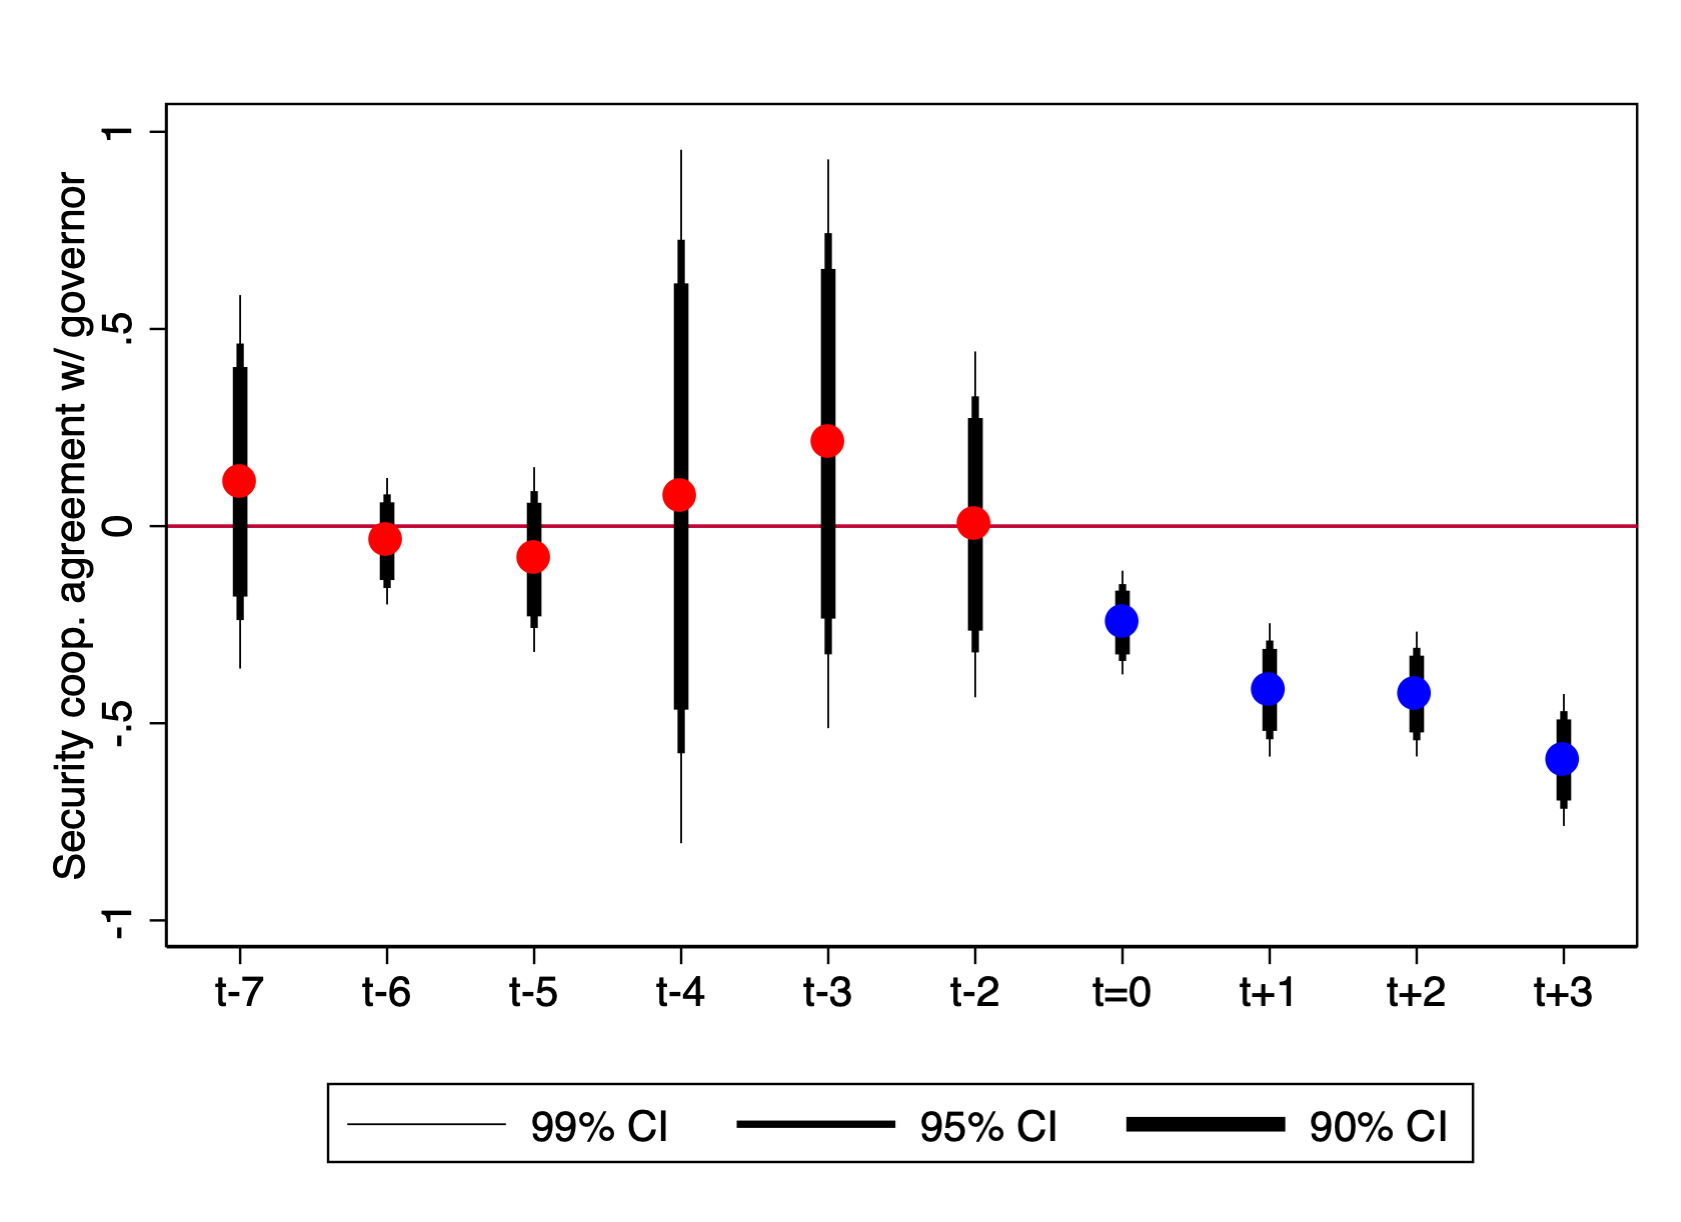
\includegraphics[width=0.9\textwidth]{../Figures/catts_agreements.png}
       \captionsetup{justification=centering}
       
 \textbf{Note:} Figure \ref{fig:event_study_agreements} shows the IW estimators following \citet{abraham_sun_2020} for each lead and lag relative to the first year a municipality implemented reelection. Red points are pre-treatment, while blue ones post-treatment. 
  
\end{figure}   
    

\section{Robustness}

Main takeaways: 

1. Results are robust across multiple specifications and models. 


\begin{table}[htbp]\def\sym#1{\ifmmode^{#1}\else\(^{#1}\)\fi}
\centering
\caption{Effect of 2014 Term Limit Reform on Signing Security Cooperation Agreements, Average Effect }
\label{tab:as_aggregate}
\scalebox{0.7}{
\begin{tabular}{lcccc}
\hline \hline
\\ \multicolumn{3}{l}{Dependent variable: Sign Security Cooperation Agreement w/ Governor}\\
Model: & CATTs & CATTs w/ WILD CIs & Change ref. period (t=0) & Trim $<$ t-4 \\
& \multicolumn{1}{c}{(1)} & \multicolumn{1}{c}{(2)} & \multicolumn{1}{c}{(3)}  & \multicolumn{1}{c}{(4)}  \\
\cmidrule(lrr){2-2}  \cmidrule(lrr){3-3}  \cmidrule(lrr){4-4} \cmidrule(lrr){5-5}\\
\addlinespace
Reform Average Effect (from t to t+3)       & $-0.4197^{***} $$ & $-0.4197 ^{***} $$ & $-0.4622 ^{**} $$ & $-0.3559 ^{***} $$   \\
& (0.0457( & (0.0473)  & (0.1977) & (0.0468)  \\
\addlinespace
Observations       &      12,173 &      12,173 &      12,173 &      12,173 \\
R-squared         & 0.4545 & 0.4545 & 0.4545 & 0.4544 \\
Mun. FEs       &     \checkmark         &  \checkmark &     \checkmark         &  \checkmark     \\
Year. FEs       &     \checkmark         &  \checkmark  &     \checkmark         &  \checkmark \\
Controls$^b$   &      \checkmark       &      \checkmark &      \checkmark       &      \checkmark    \\
Cohort weighted   &   \checkmark       &   \checkmark  &   \checkmark       &   \checkmark  \\
Parallel trend holds   &   \checkmark       &   \checkmark  &   \checkmark       &   \checkmark   \\
\hline \hline
\multicolumn{5}{p{1.3\textwidth}}{\footnotesize{Notes: Coefficients show IW estimators following \citet{abraham_sun_2020}. Two relative time periods (lag 8 and 1) are removed to avoid collinearity problems noted by \citet{abraham_sun_2020} except for the specification that trims periods prior to t-4. Standard errors in parentheses are clustered at the state level, with the following significance-level: $^{***}$ 1\%; $^{**}$ 5\%; and $^*$ 10\%, that refer to two-sided t-test with the null hypothesis equal to 0 for each relative time period. $^b$ State-level controls include governor winning margin in last pre-treatment election and an indicator of whether the governor's party is the same as the federal incumbent party.}} \\
\end{tabular}
}
\end{table}
  

\begin{figure}[H]   
\centering
 \caption{Effect of Term Limit Reform on Security Cooperation Agreements signed with the Governor, 2010-2018}
 \label{fig:robustness_agreements}
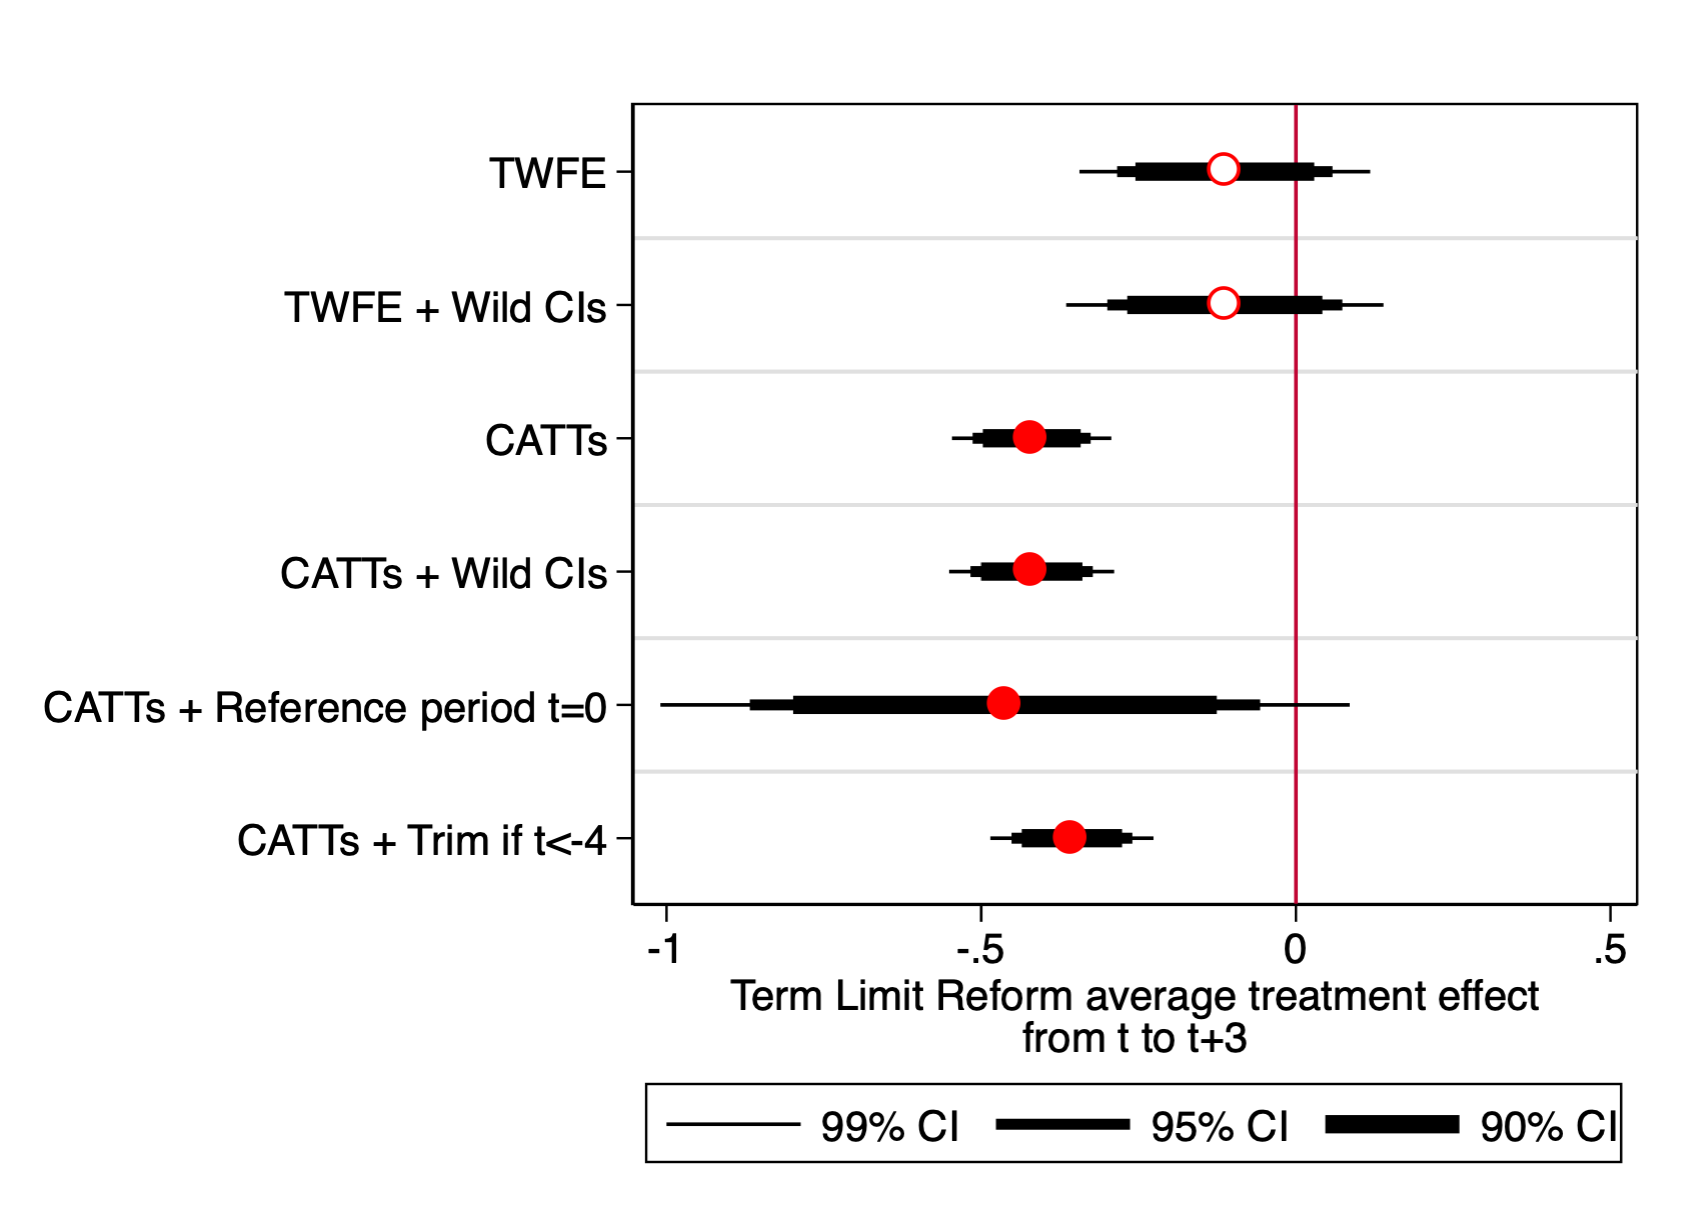
\includegraphics[width=0.9\textwidth]{../Figures/average_effects.png}
       \captionsetup{justification=centering}
       
 \textbf{Note:} Figure \ref{fig:robustness_agreements} shows the average treatment effect from t to t+3 across multiple specifications. This average effect was estimated using the IW estimators following \citet{abraham_sun_2020} for each lead and lag relative to the first year a municipality implemented reelection. Red points show that parallel trends hold, while hollow ones imply pretrends. 
\end{figure}   

2. Results only present if upper-level government can compete in credit claiming locally (President never does this). 

 \begin{figure}[H]   
\centering
 \caption{Comparison: Security Cooperation Agreements with Governor vs. Other Actors, 2014-2018}
 \label{fig:comparison_fed_estatal}
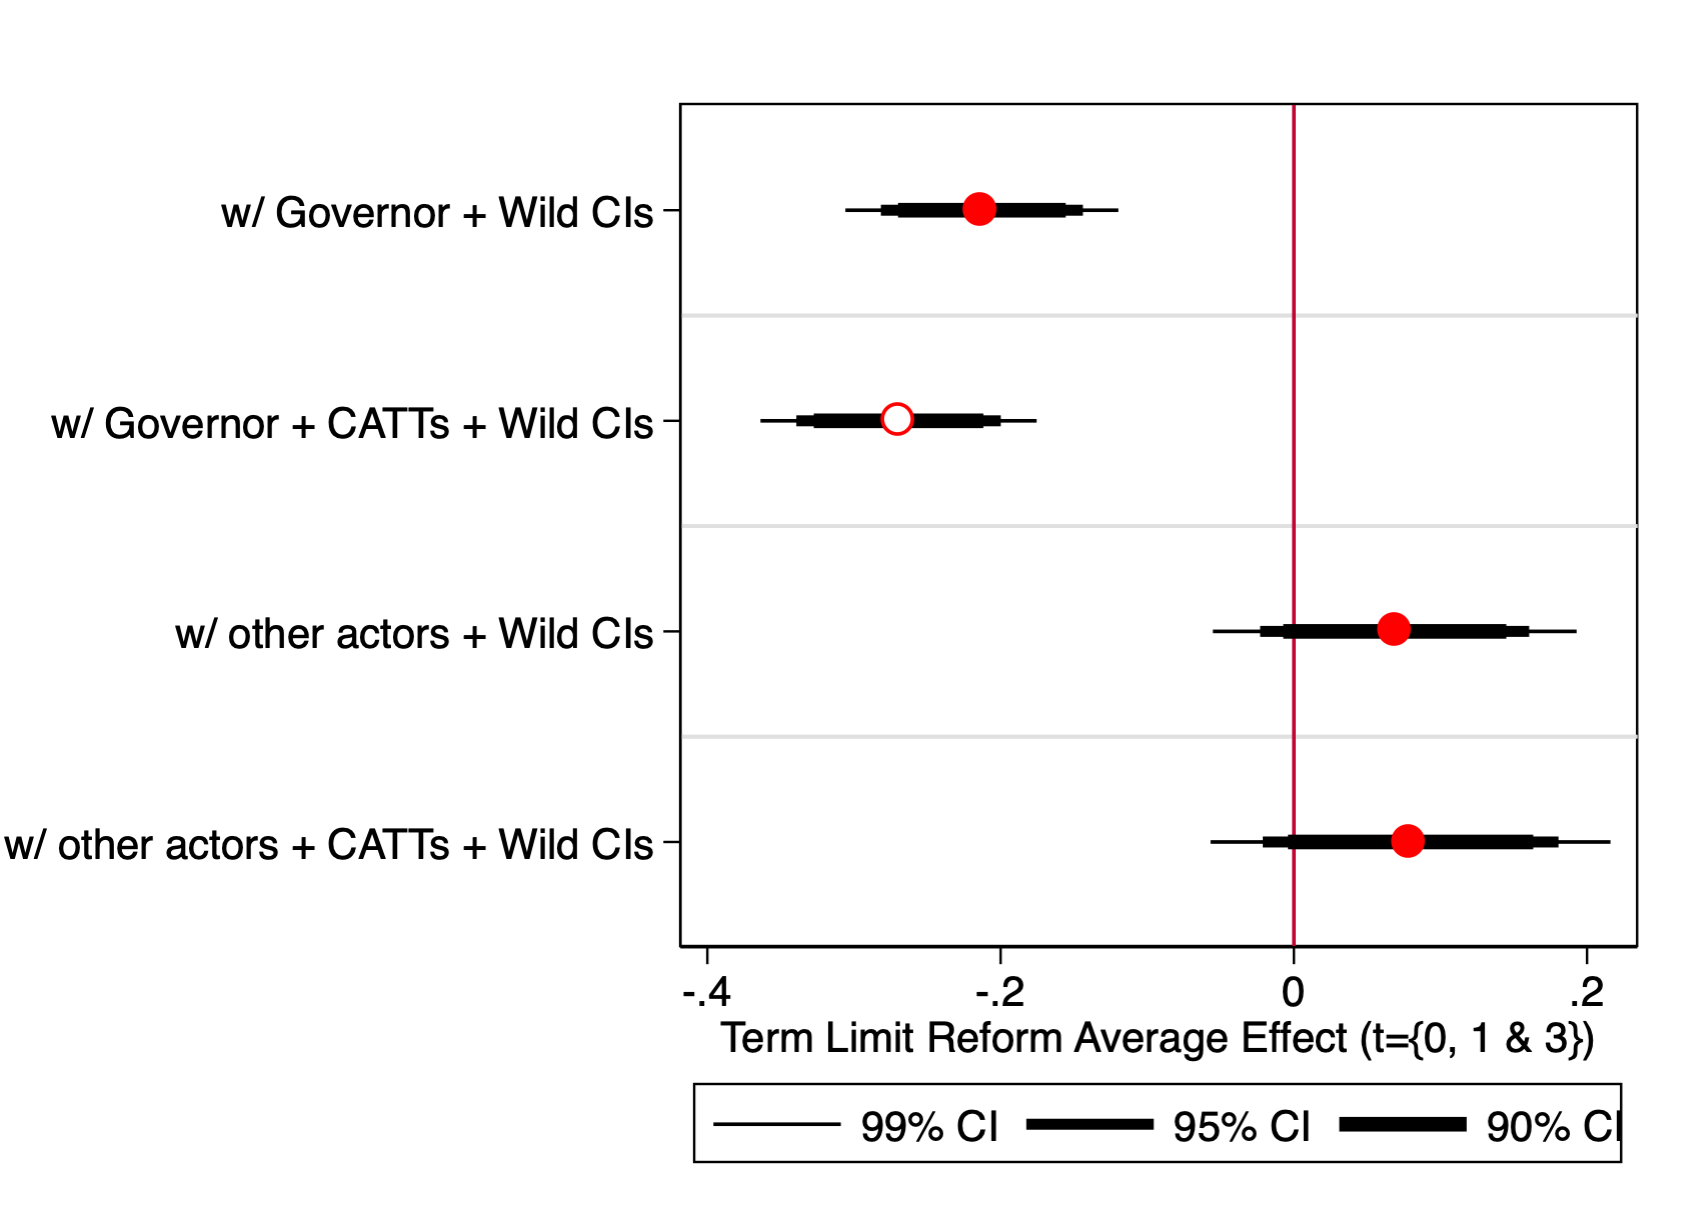
\includegraphics[width=0.9\textwidth]{../Figures/average_effects_comparisonfedest.png}
       \captionsetup{justification=centering}
       
 \textbf{Note:} Figure \ref{fig:comparison_fed_estatal} shows the average treatment effect from t to t+3 across multiple specifications. This average effect was estimated using the IW estimators following \citet{abraham_sun_2020} for each lead and lag relative to the first year a municipality implemented reelection. Red points show that parallel trends hold, while hollow ones imply pretrends. 
\end{figure}   

\clearpage 



\section{Mechanisms}

Main takeaways: 

%Pull strategy:

1. Mayors facing reelection decrease the delegation of public security provision and traffic, but not other services. 

 \begin{figure}[H]   
\centering
 \caption{Comparison: Security Cooperation Agreements with Governor vs. Other Actors, 2014-2018}
 \label{fig:services}
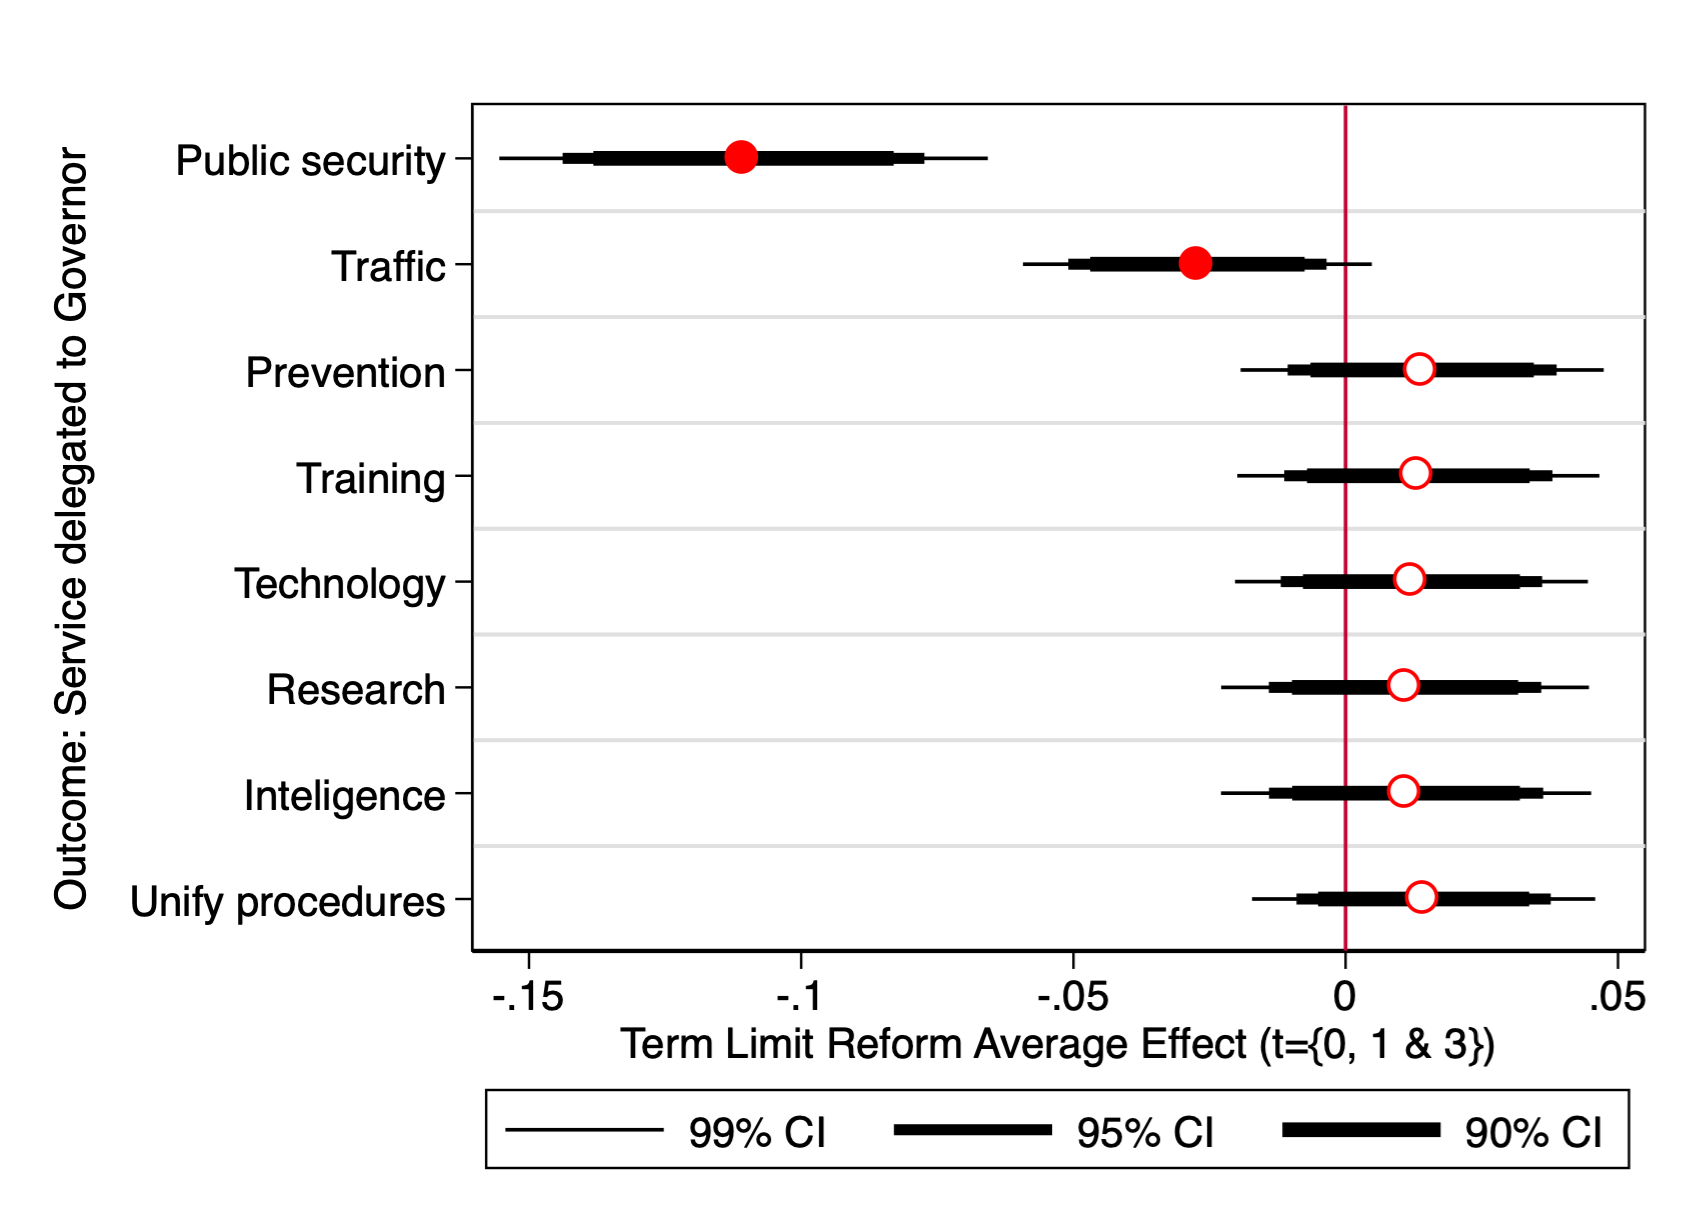
\includegraphics[width=0.9\textwidth]{../Figures/services.png}
       \captionsetup{justification=centering}
       
 \textbf{Note:} Figure \ref{fig:services} shows the average treatment effect from t, t+1 and t+3 across multiple specifications. This average effect was estimated using the IW estimators following \citet{abraham_sun_2020} for each lead and lag relative to the first year a municipality implemented reelection. Red points show that parallel trends hold, while hollow ones imply pretrends. 
\end{figure}   

\clearpage
2. Alignment: If you are aligned you have a lot to loose in terms of credit claim, especially if you are from the PRI. This should be smaller for alignment with President since you are not competing directly in terms of reputation in local politics. Lastly, we should see a greater negative effect if not aligned since citizens do not blame you as much por public security inefficiencies following \citet{ley_2017}.

\begin{figure}[H]   
\centering
 \caption{Reform interaction with Party Alignment}
 \label{fig:alignment}
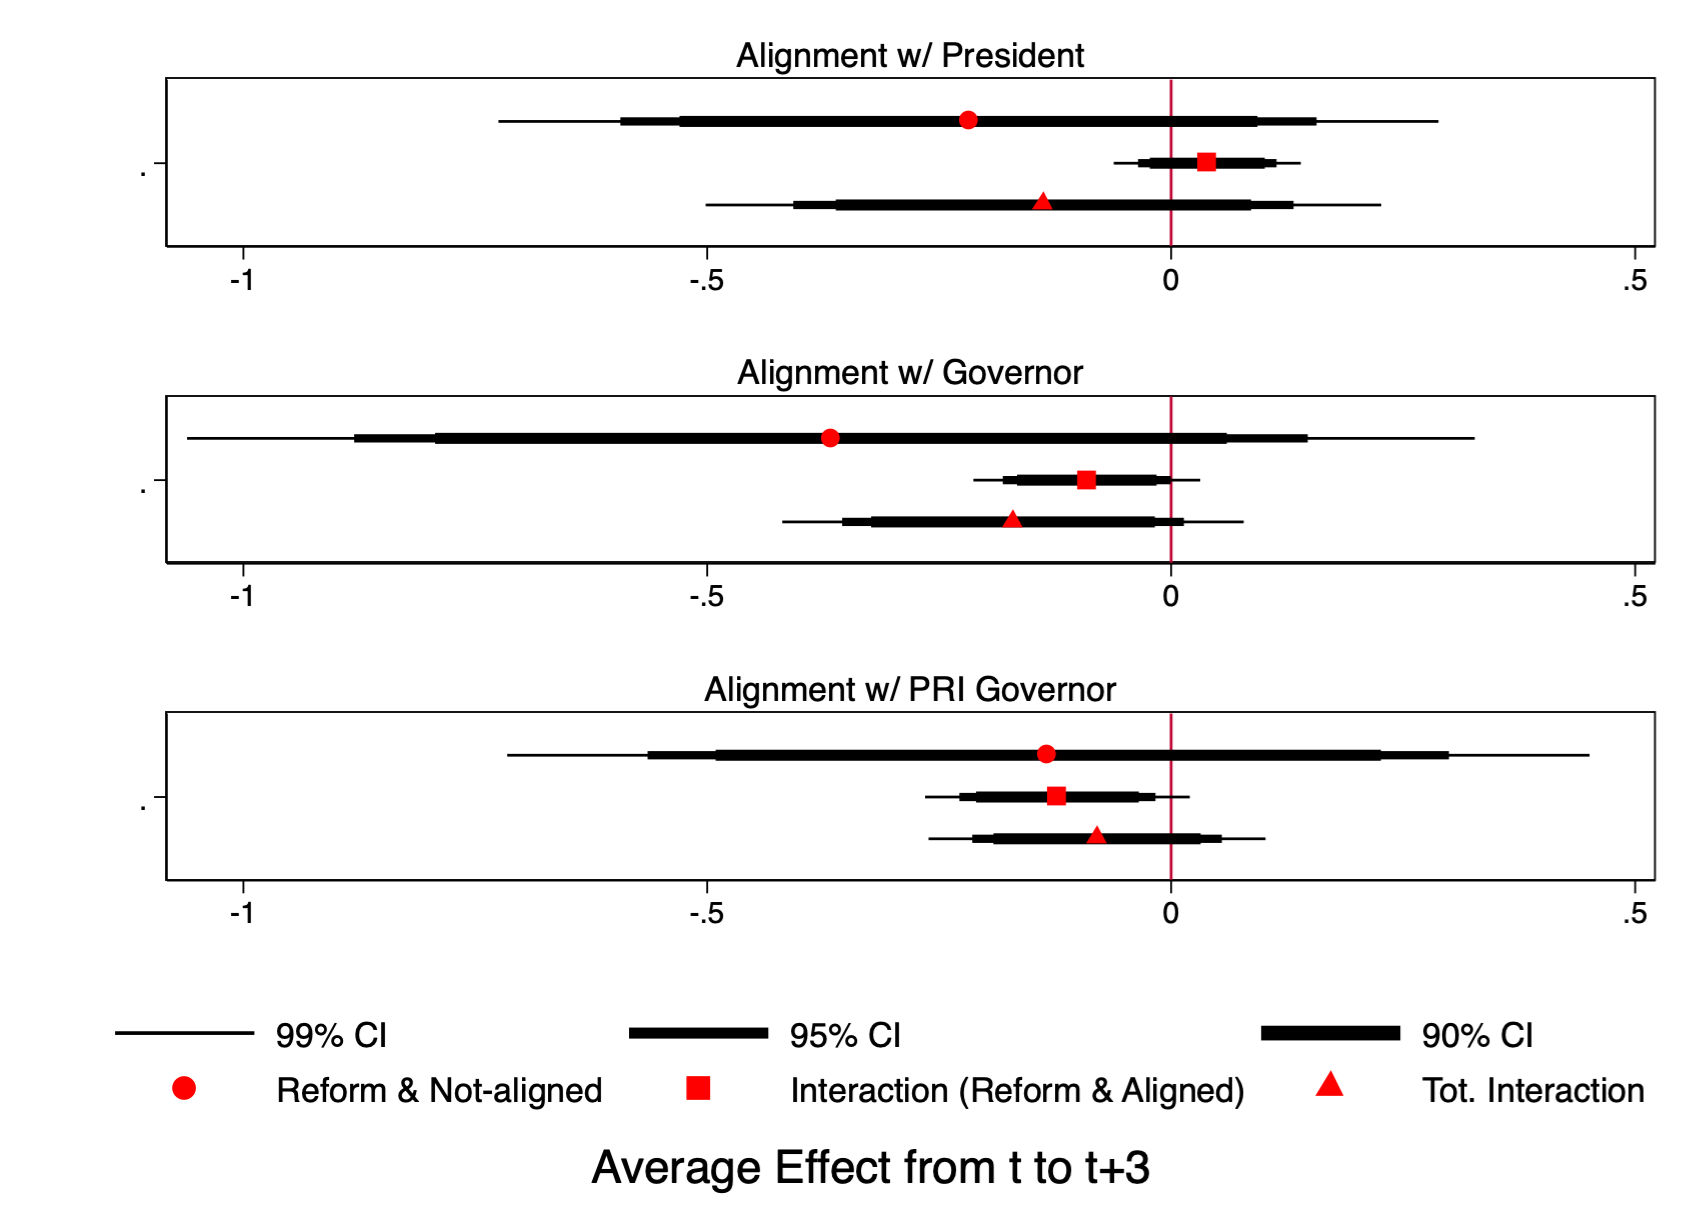
\includegraphics[width=0.9\textwidth]{../Figures/interaction_alignment_full.png}
       \captionsetup{justification=centering}
       
 \textbf{Note:} Figure \ref{fig:alignment} shows the average treatment effect from t to t+3 across multiple specifications. This average effect was estimated using the IW estimators following \citet{abraham_sun_2020} for each lead and lag relative to the first year a municipality implemented reelection. Red points show that parallel trends hold, while hollow ones imply pretrends. To check parallel trends see Appendix Figure \ref{tab:interaction_alignment}.  
\end{figure}  

\clearpage
3. a. Mayors facing reelection want to show responsiveness to constituents preferences. 
3. b. Mayors facing reelection sign security agreements when faced by problems "too big" or of the national order. 

\begin{figure}[H]   
\centering
 \caption{Interaction effects by citizens' preferences}
 \label{fig:preferences}
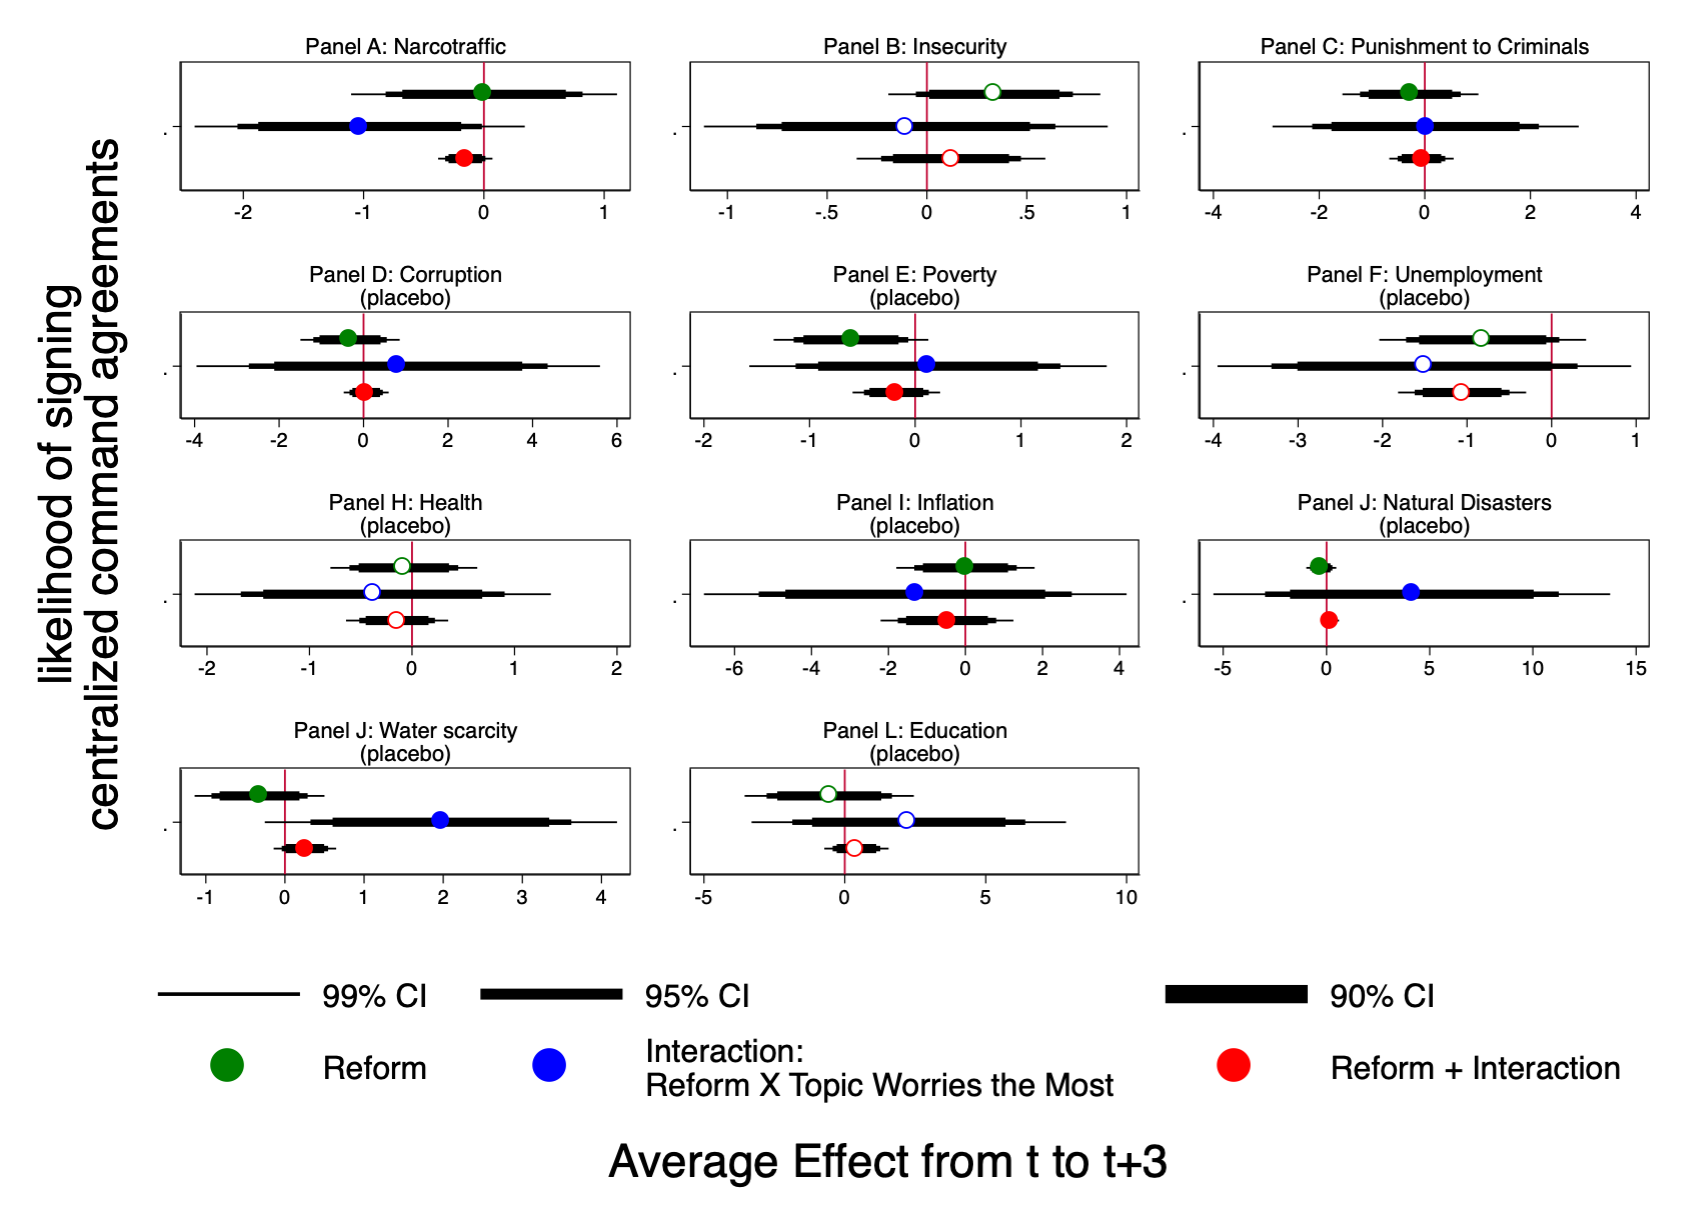
\includegraphics[width=1\textwidth]{../Figures/preferences.png}
       \captionsetup{justification=centering}
       
 \textbf{Note:} Figure \ref{fig:preferences} shows the average treatment effect from t to t+3 across multiple specifications. This average effect was estimated using the IW estimators following \citet{abraham_sun_2020} for each lead and lag relative to the first year a municipality implemented reelection. Filled points show that parallel trends hold, while hollow ones imply pretrends.  
\end{figure} 
  
  \clearpage
%Push strategy:
4. Mayors facing reelection do not sign agreements when other security forces are highly trusted or identified.

\begin{figure}[H]   
\centering
 \caption{Total interaction effects by citizens' trust and identification of police forces}
 \label{fig:trust_identify}
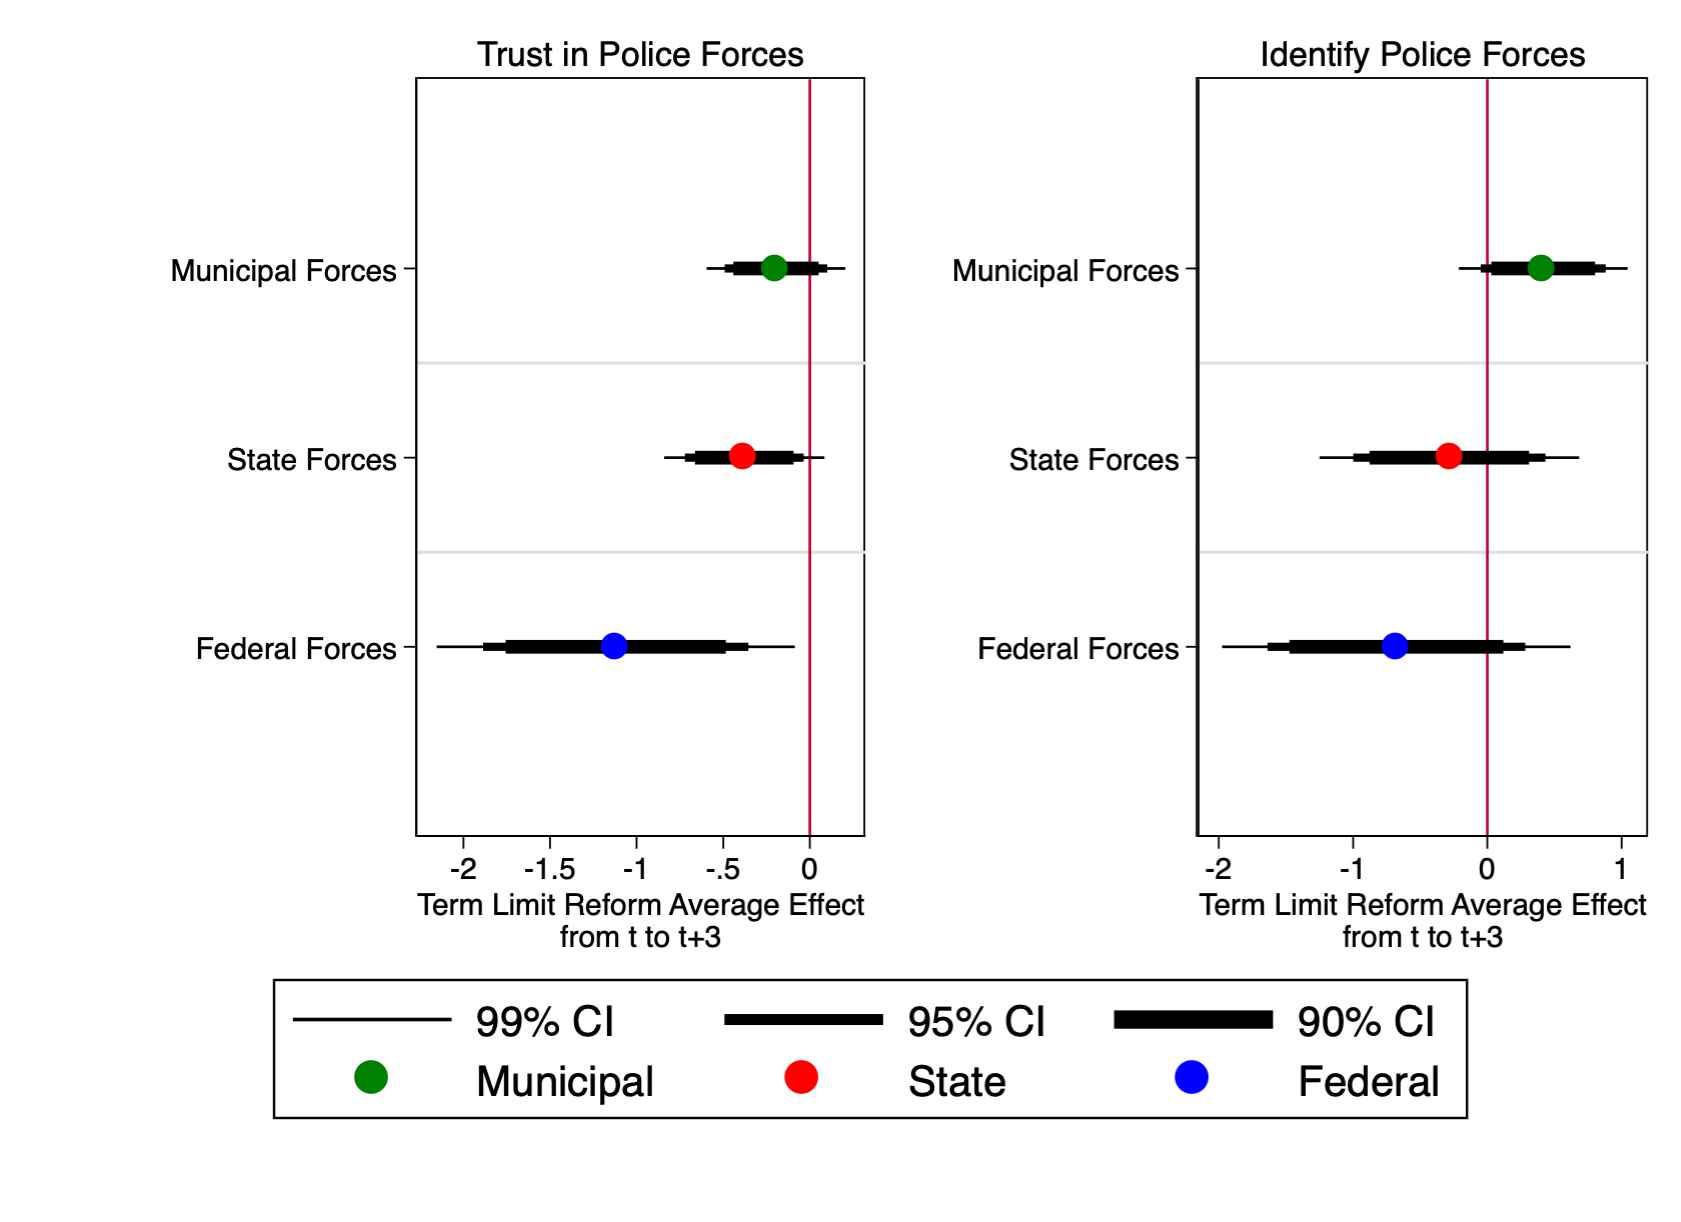
\includegraphics[width=1\textwidth]{../Figures/trust&preferences.png}
       \captionsetup{justification=centering}
       
 \textbf{Note:} Figure \ref{fig:trust_identify} shows the average treatment effect from t to t+3 across multiple specifications. This average effect was estimated using the IW estimators following \citet{abraham_sun_2020} for each lead and lag relative to the first year a municipality implemented reelection. Filled points show that parallel trends hold, while hollow ones imply pretrends.       
\end{figure}   
   
  

\clearpage
\section{Ruling out Alternative Hypothesis}
\subsection{Selection: incumbents and challengers quality}
\subsection{Cartel Presence}

All regressions control for Cartel Presence pretreatment. 

\subsection{Citizens' Evaluation of Corruption and Efficiency of Police Forces}

\begin{figure}[H]   
\centering
 \caption{Interaction effects by citizens' evaluation of efficiency and corruption of police forces}
 \label{fig:efficiency_corruption}
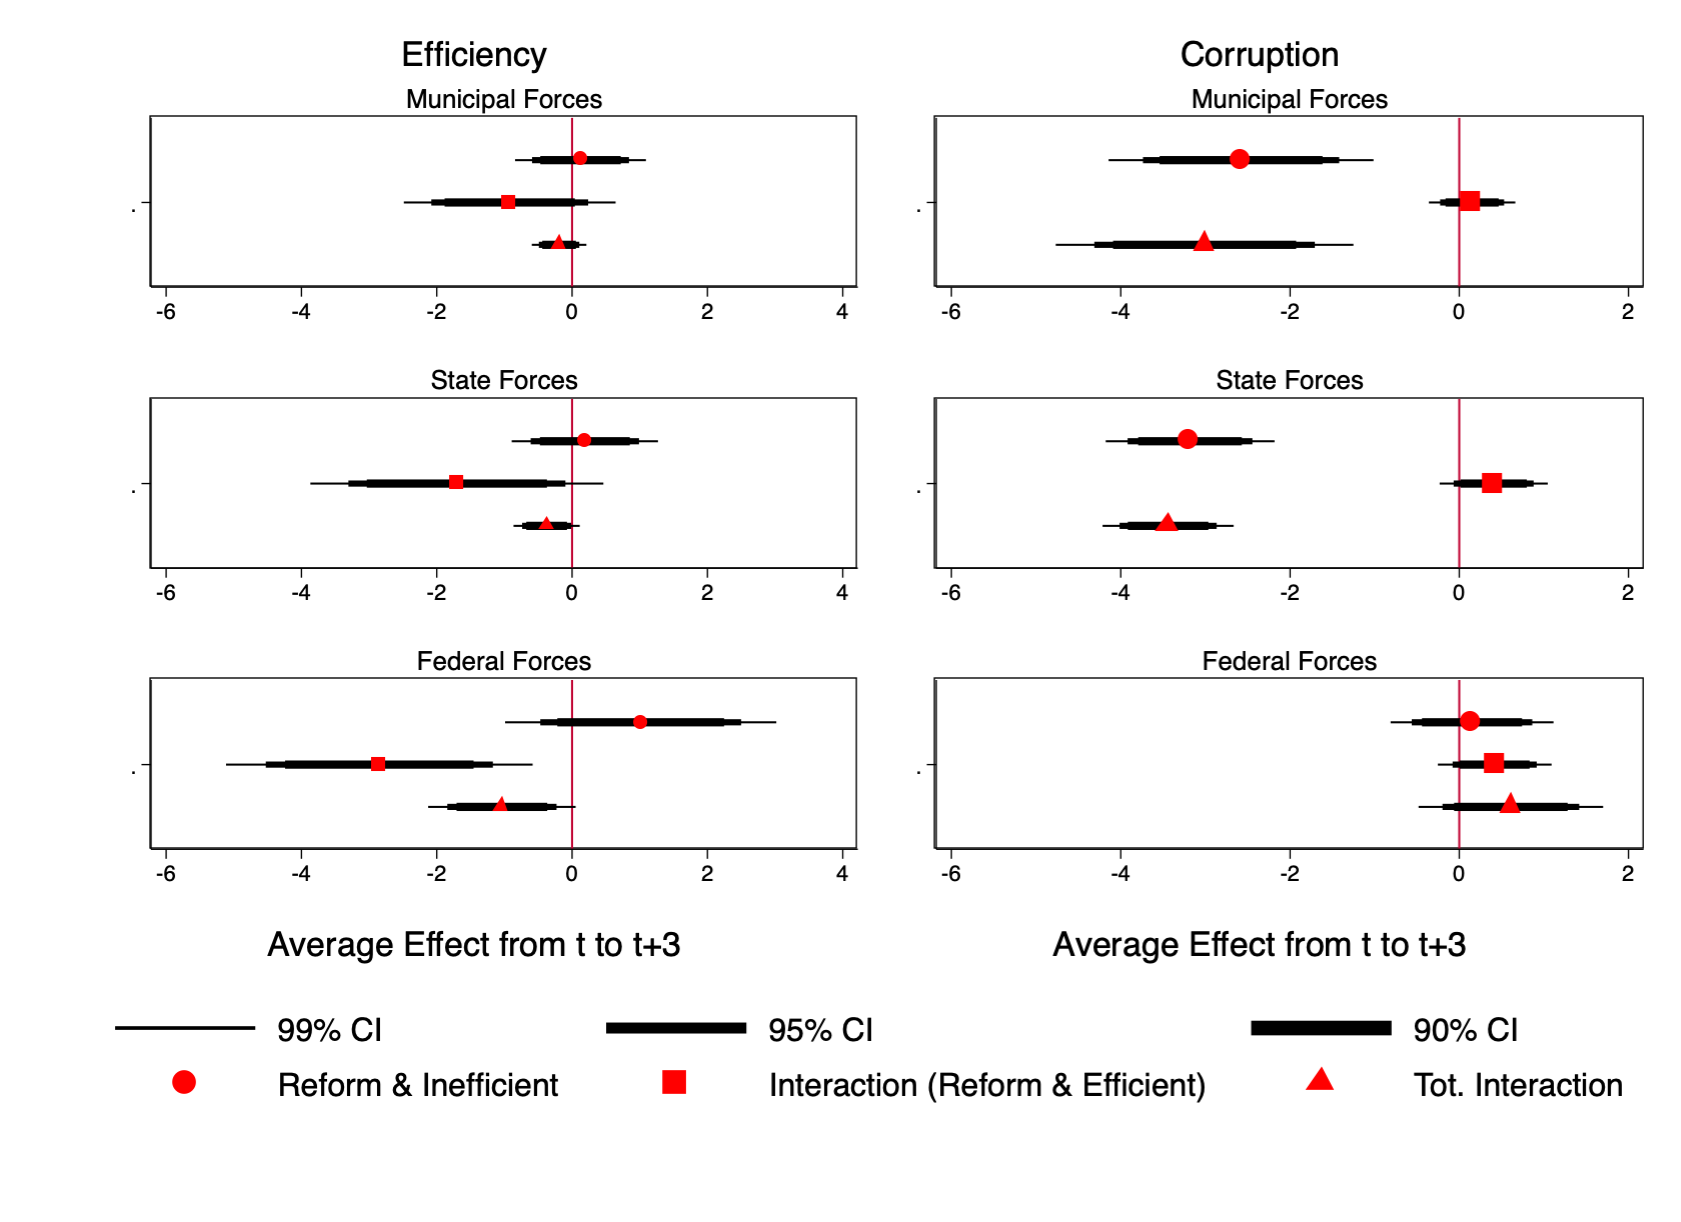
\includegraphics[width=1\textwidth]{../Figures/efficiency_corruption.png}
       \captionsetup{justification=centering}
         
 \textbf{Note:} Figure \ref{fig:efficiency_corruption} shows the average treatment effect from t to t+3 across multiple specifications. This average effect was estimated using the IW estimators following \citet{abraham_sun_2020} for each lead and lag relative to the first year a municipality implemented reelection. Filled points show that parallel trends hold, while hollow ones imply pretrends.        
\end{figure}  

\clearpage

\section{Unintended consequences}

\subsection{Preferences for order and security}
1. PREFERENCES: citizens are more concerned about security but less about other things. Recall results are conditional on violence. So in the next election, they will look for another hawk. This ties to the incumbency advantage.

\begin{figure}[H]   
\centering
 \caption{Effect of Term Limit Reform on Citizens' Preferences}
 \label{fig:preferences}
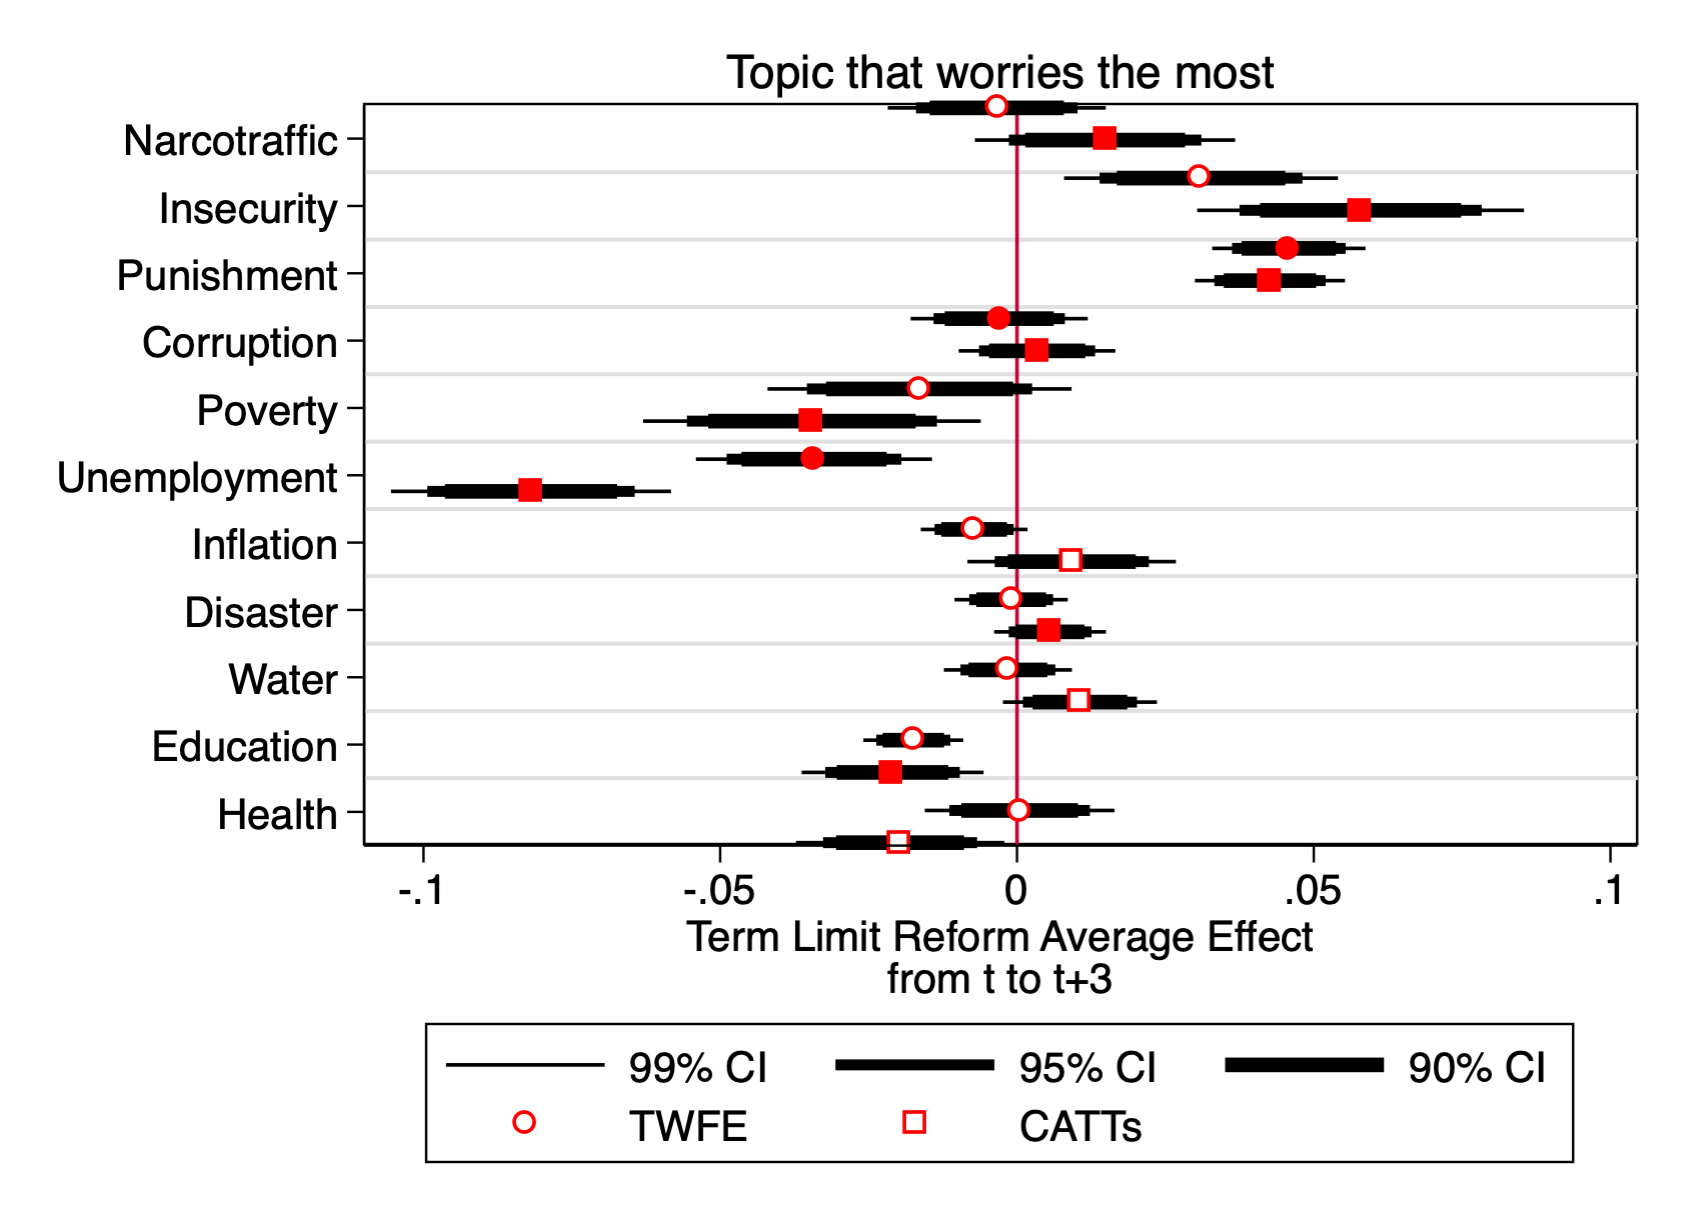
\includegraphics[width=1\textwidth]{../Figures/change_preferences_comparison.png}
       \captionsetup{justification=centering}
         
 \textbf{Note:} Figure \ref{fig:preferences} shows the average treatment effect from t to t+3 across multiple specifications. This average effect was estimated using the IW estimators following \citet{abraham_sun_2020} for each lead and lag relative to the first year a municipality implemented reelection. Filled points (squares) show that parallel trends hold, while hollow ones imply pretrends.        
\end{figure}   
 

\subsection{Security underprovision and violence}
3. VIOLENCE: increase of violence.


\begin{figure}[H] 
\centering
 \caption{Effect of Term Limit Reform on Violence}
 \label{fig:as_violence}
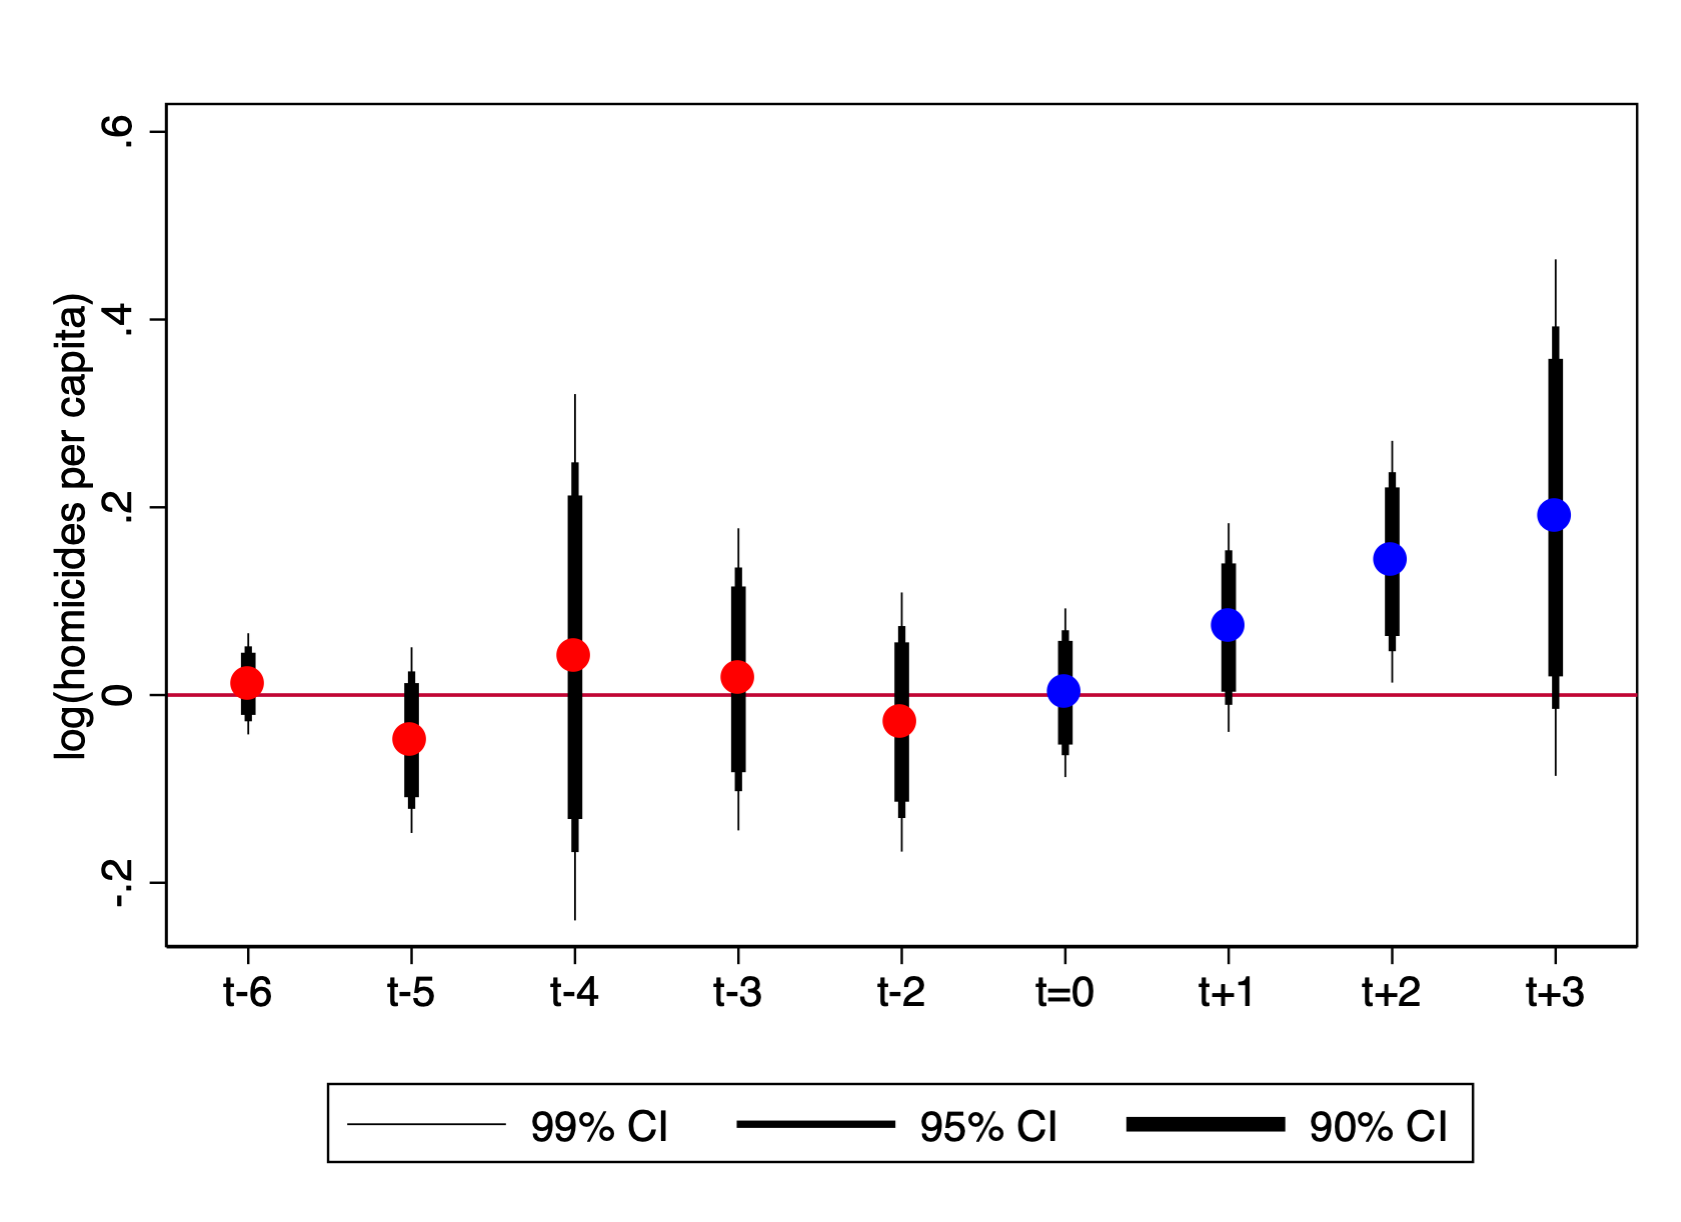
\includegraphics[width=0.9\textwidth]{../Figures/catts_homicides.png}
       \captionsetup{justification=centering}
       
 \textbf{Note:} Figure \ref{fig:as_violence} shows the IW estimators following \citet{abraham_sun_2020} for each lead and lag relative to the first year a municipality implemented reelection. Red points are pre-treatment, while blue ones post-treatment. 
    
\end{figure}    

\begin{table}[H]\def\sym#1{\ifmmode^{#1}\else\(^{#1}\)\fi}
\centering
\caption{Effect of Security Cooperation Agreements signed with the Governor on Violence}
\label{tab:2sls_agreement_violence}
\scalebox{1}{
\begin{tabular}{l*{2}{c}}
\hline \hline
  &\multicolumn{1}{c}{(1)}         &\multicolumn{1}{c}{(2)}         \\
\addlinespace
Predicted Agreement w/ Governor&     -0.1521\sym{*}  &     -0.1521\sym{**} \\
            &    (0.0802)         &    (0.0749)         \\
\addlinespace
Observations&      12,173         &      12,173         \\
R2          &       0.724         &       0.724         \\
Controls$^a$    &  \checkmark         &  \checkmark         \\
Mun. FE     &  \checkmark         &  \checkmark         \\
Year FE     &  \checkmark         &  \checkmark         \\
State Cluster S.E.&                     &  \checkmark         \\
Wild CI$^b$     &                     &  \checkmark         \\
First stage F-stat      &        1,739         &        1,739         \\
\hline \hline
\multicolumn{3}{p{0.7\textwidth}}{\footnotesize{Notes: Coefficients show IW estimators following \citet{abraham_sun_2020}. Two relative time periods (lag 8 and 1) were removed to avoid collinearity problems noted by \citet{abraham_sun_2020}. Standard errors in parentheses are clustered at the state level unless indicated, with the following significance-level: $^{***}$ 1\%; $^{**}$ 5\%; and $^*$ 10\%, that refer to two-sided t-test with the null hypothesis equal to 0 for each relative time period.  $^a$ Pretreatment controls include: governor winning margin; party alignment with the President;  party alignment with the Governor; municipal winning margin; and Cartel presence. $^a$ Wild bootstrap standard errors clustered at the state-level are reported when indicated.}} \\
\end{tabular}
}
\end{table} 



\begin{figure}[h]  
\centering
\caption{Effect of Term Limit Reform on Effort of Local and Federal Security Forces} 
\label{fig:effort}

   
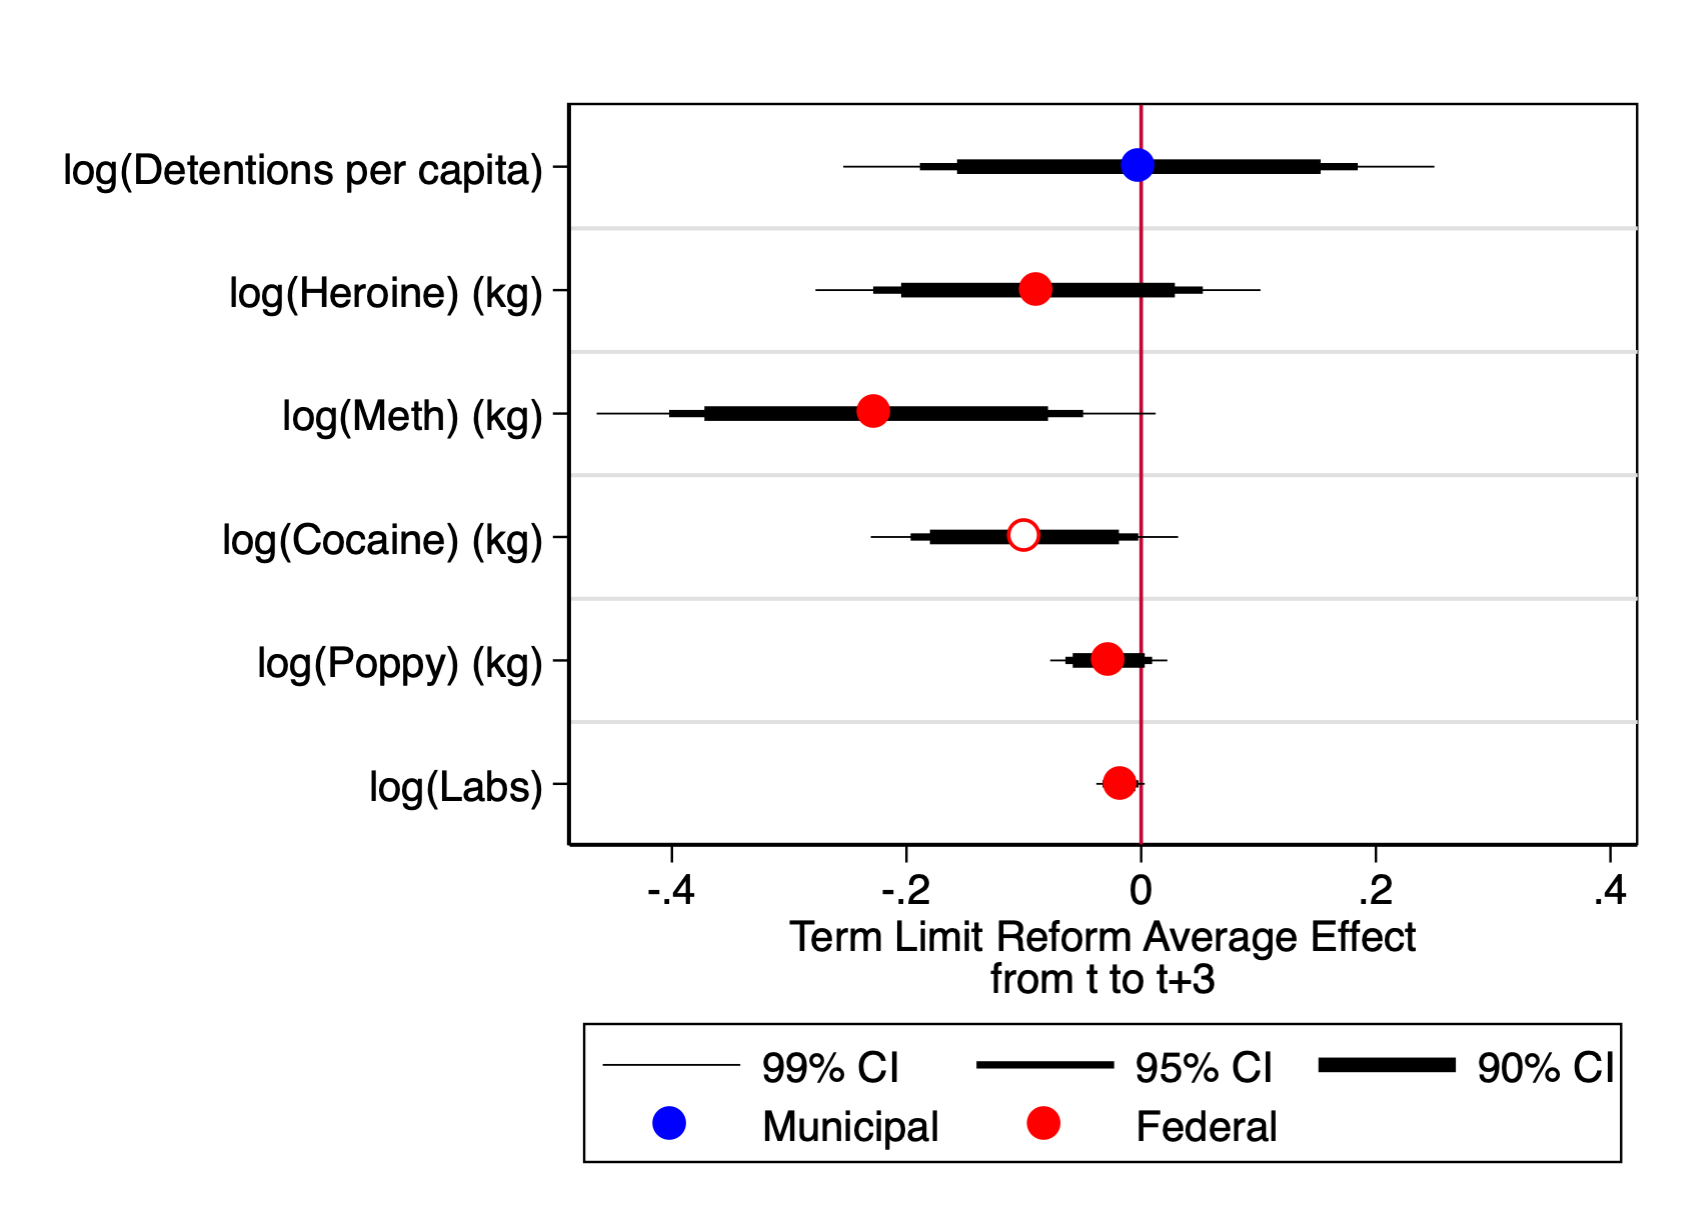
\includegraphics[width=1\textwidth]{../Figures/effort.png}
  
 \textbf{Note:} Figure \ref{fig:effort} shows the average treatment effect from t to t+3 across multiple specifications. This average effect was estimated using the IW estimators following \citet{abraham_sun_2020} for each lead and lag relative to the first year a municipality implemented reelection. Filled points show that parallel trends hold, while hollow ones imply pretrends.        
\end{figure} 


\clearpage
\section{New Appendix}

\subsection{Main Results}
\begin{table}[H]\def\sym#1{\ifmmode^{#1}\else\(^{#1}\)\fi}
\centering
\caption{Effect of 2014 Term Limit Reform on Security Cooperation Agreements signed with the Governor, 2010-2018}
\label{tab:as_agreements}
\scalebox{0.75}{
\begin{tabular}{lcc}
\hline \hline
\\ \multicolumn{3}{l}{Dependent variable:}\\
& \multicolumn{2}{c}{Security Cooperation Agreement} \\
& \multicolumn{2}{c}{w/ Governor$^{a}$} \\

& \multicolumn{1}{c}{(1)} & \multicolumn{1}{c}{(2)} \\
\cmidrule(lrr){2-2}  \cmidrule(lrr){3-3}\\
\addlinespace
Lag 7 years &      $ 0.1123^{} $ &  $ 0.1123^{} $   \\
& ($ 0.1709$) & ($ 0.7117 $) \\
Lag 6 years &          $ -0.0383^{} $ &   $ -0.0383^{} $  \\
& ($ 0.0579$) & ($ 0.2458 $) \\
Lag 5 years &        $ -0.0848^{} $ &   $ -0.0848^{} $ \\
& ($ 0.0846$) & ($ 0.2404 $) \\
Lag 4 years &         $ 0.0751^{} $ &      $ 0.0751^{} $  \\
& ($ 0.3174$) & ($ 0.2890 $) \\
Lag 3 years &        $ 0.2088^{} $ &     $ 0.2088^{} $ \\
& ($ 0.2603$) & ($ 0.2139 $) \\
Lag 2 years &        $ 0.0044^{} $ &    $ 0.0044^{} $  \\
& ($ 0.1583$) & ($ 0.2139 $) \\
Reform, time 0 &        $ -0.2446^{***} $ &     $ -0.2446^{***} $ \\
& ($ 0.0475$) & ($ 0.0685 $) \\
Lead 1 year &         $ -0.4154^{***} $ &       $ -0.4154^{***} $ \\
& ($ 0.0610$) & ($ 0.0610 $) \\
Lead 2 years &         $ -0.4259^{***} $ &      $ -0.4259^{***} $  \\
& ($ 0.0571$) & ($ 0.0571 $) \\
Lead 3 years &        $ -0.5931^{***} $ &     $ -0.5931^{***} $ \\
& ($ 0.0604$) & ($ 0.0604 $) \\
\addlinespace
Observations       &                 12,173        &          12,173  \\
R-squared        &              0.4545        &           0.4545   \\
Mun. FEs       &     \checkmark         &  \checkmark    \\
Year. FEs       &     \checkmark         &  \checkmark   \\
Controls$^b$   &      \checkmark       &      \checkmark    \\
Cohort weighted   &   \checkmark       &   \checkmark    \\
WILD CI   &          &   \checkmark    \\
Aggregate effect        &           $   -0.4197^{***} $        &           $-0.4197^{***} $    \\
SE (aggregate eff.)        &              0.0457        &           0.0473   \\
\hline \hline
\multicolumn{3}{p{0.6\textwidth}}{\footnotesize{Notes: Coefficients show IW estimators following \citet{abraham_sun_2020}. Two relative time periods (lag 8 and 1) are removed to avoid collinearity problems noted by \citet{abraham_sun_2020}. Standard errors in parentheses are clustered at the state level, with the following significance-level: $^{***}$ 1\%; $^{**}$ 5\%; and $^*$ 10\%, that refer to two-sided t-test with the null hypothesis equal to 0 for each relative time period. $^a$ Refers to security cooperation agreements signed with the Governor. $^b$ Pretreatment controls include: governor winning margin; party alignment with the President;  party alignment with the Governor; municipal winning margin; logged population; logged organized crime related deaths; and Cartel presence.}} \\
\end{tabular}
} 
\end{table}
    
 
\subsection{Robustness}

\begin{table}[htbp]\def\sym#1{\ifmmode^{#1}\else\(^{#1}\)\fi}
\centering
\caption{Effect of 2014 Term Limit Reform on the likelihood of signing Security Cooperation Agreements, \citet{chaisemarting_etal_2019} correction}
\label{tab:chaisemartin_agreements}
\scalebox{1}{
\begin{tabular}{lcc}
\hline \hline
\\ \multicolumn{3}{l}{Dependent variable:}\\
& \multicolumn{1}{c}{Agreement A} & \multicolumn{1}{c}{Agreement B$^{a}$} \\
& \multicolumn{1}{c}{(1)} & \multicolumn{1}{c}{(2)} \\
\cmidrule(lrr){2-2}  \cmidrule(lrr){3-3}\\
\addlinespace
t-6 &          $ -0.0645^{} $ &   $ -0.0645^{} $  \\
& ($ 0.0399$) & ($ 0.8961 $) \\
t-5 &        $ -0.2071^{**} $ &   $ -0.2071^{} $ \\
& ($ 0.0751$) & ($ 2.6703 $) \\
t-4 &         $ -0.0712^{} $ &      $ -0.0712^{} $  \\
& ($ 0.1733$) & ($ 1.2658 $) \\
t-3 &        $ 0.1037^{} $ &     $ 0.1037^{} $ \\
& ($ 0.1362$) & ($ 0.3138 $) \\
t-2 &        $ -0.0251^{} $ &    $ -0.0251^{} $  \\
& ($ 0.1157$) & ($ 0.3138 $) \\
t-1 &        $ -0.0738^{} $ &     $ -0.0738^{} $ \\
& ($ 0.0918$) & ($ 1.6557 $) \\
t+1 &         $ -0.2837^{} $ &       $ -0.2837^{} $ \\
& ($ 0.2012$) & ($ 0.2012 $) \\
t+2 &         $ -0.6165^{**} $ &      $ -0.6165^{**} $  \\
& ($ 0.2330$) & ($ 0.2330 $) \\
t+3 &        $ -0.4813^{*} $ &     $ -0.4813^{*} $ \\
& ($ 0.2641$) & ($ 0.2641 $) \\
\addlinespace
Observations       &                 12,173        &          12,173  \\
R-squared        &              0.4542        &           0.4542   \\
Mun. FEs       &     \checkmark         &  \checkmark    \\
Year. FEs       &     \checkmark         &  \checkmark   \\
Controls$^b$   &      \checkmark       &      \checkmark    \\
Cohort weighted   &   \checkmark       &   \checkmark    \\
WILD CI   &          &   \checkmark    \\
Aggregate effect        &              -0.4605        &           -0.4605   \\
SE (aggregate eff.)        &              0.1973        &           0.1973   \\
p-value(aggregate eff.)       &              0.0273        &           0.0273   \\
\hline \hline
\multicolumn{3}{p{0.8\textwidth}}{\footnotesize{Notes: Coefficients show IW estimators following \citet{abraham_sun_2020}. Two relative time periods (lag 8 and 1) are removed to avoid collinearity problems noted by \citet{abraham_sun_2020}. Standard errors in parentheses are clustered at the state level, with the following significance-level: $^{***}$ 1\%; $^{**}$ 5\%; and $^*$ 10\%, that refer to two-sided t-test with the null hypothesis equal to 0 for each relative time period. $^a$ Refers to the inverse hyperbolic sine transformation. $^b$ State-level controls include governor winning margin in last pre-treatment election and an indicator of whether the governor's party is the same as the federal incumbent party.}} \\
\end{tabular}
}
\end{table}
  
    
 \begin{table}[htbp]\def\sym#1{\ifmmode^{#1}\else\(^{#1}\)\fi}
\centering
\caption{Effect of Term Limit Reform on Security Cooperation Agreements signed with the Governor, trimming periods}
\label{tab:as_agreements_trim}
\scalebox{1}{
\begin{tabular}{lcc}
\hline \hline
\\ \multicolumn{3}{l}{Dependent variable:}\\
& \multicolumn{2}{c}{Security Cooperation Agreement} \\
& \multicolumn{2}{c}{w/ Governor$^{a}$} \\
& \multicolumn{1}{c}{(1)} & \multicolumn{1}{c}{(2)} \\
\cmidrule(lrr){2-2}  \cmidrule(lrr){3-3}\\
\addlinespace
t-4 years &         $ 0.1961^{} $ &      $ 0.1961^{} $  \\
& ($ 0.2680$) & ($ 0.8260 $) \\
t-3 &        $ 0.2193^{} $ &     $ 0.2193^{} $ \\
& ($ 0.2070$) & ($ 0.2702 $) \\
t-2 &        $ 0.0370^{} $ &    $ 0.0370^{} $  \\
& ($ 0.1546$) & ($ 0.2702 $) \\
t=0 (Reform) &        $ -0.3057^{***} $ &     $ -0.3057^{} $ \\
& ($ 0.0682$) & ($ 0.4093 $) \\
t+1 &         $ -0.2858^{***} $ &       $ -0.2858^{} $ \\
& ($ 0.0725$) & ($ 0.2610 $) \\
t+2 &         $ -0.2389^{***} $ &      $ -0.2389^{} $  \\
& ($ 0.0823$) & ($ 0.2369 $) \\
t+3  &        $ -0.5931^{***} $ &     $ -0.5931^{***} $ \\
& ($ 0.0604$) & ($ 0.0715 $) \\
\addlinespace
Observations       &                 12,173        &          12,173  \\
R-squared        &              0.4544        &           0.4544   \\
Mun. FEs       &     \checkmark         &  \checkmark    \\
Year. FEs       &     \checkmark         &  \checkmark   \\
Controls$^b$   &      \checkmark       &      \checkmark    \\
Cohort weighted   &   \checkmark       &   \checkmark    \\
WILD CI   &   \checkmark       &   \checkmark    \\
Aggregate effect        &              $-0.3559^{***} $     &          $ -0.3559^{**} $     \\
SE (aggregate eff.)        &              0.0468        &           0.1395   \\
\hline \hline
\multicolumn{3}{p{0.6\textwidth}}{\footnotesize{Notes: Coefficients show IW estimators following \citet{abraham_sun_2020}. I trimmed the periods lag 8, 7, 6 and 5, and removed the period 1 to avoid collinearity problems noted by \citet{abraham_sun_2020}. Standard errors in parentheses are clustered at the state level, with the following significance-level: $^{***}$ 1\%; $^{**}$ 5\%; and $^*$ 10\%, that refer to two-sided t-test with the null hypothesis equal to 0 for each relative time period. $^a$ Refers to security cooperation agreements signed with the Governor. $^b$ Pretreatment controls include: governor winning margin; party alignment with the President;  party alignment with the Governor; municipal winning margin; logged population; logged organized crime related deaths; and Cartel presence.}} \\
\end{tabular}
}
\end{table}
  

  \begin{table}[htbp]\def\sym#1{\ifmmode^{#1}\else\(^{#1}\)\fi}
\centering
\caption{Effect of 2014 Term Limit Reform on the likelihood of signing Security Cooperation Agreements}
\label{tab:chaisemartin}
\scalebox{1}{
\begin{tabular}{lcc}
\hline \hline
\\ \multicolumn{3}{l}{Dependent variable:}\\
& \multicolumn{1}{c}{Agreement A} & \multicolumn{1}{c}{Agreement B$^{a}$} \\
& \multicolumn{1}{c}{(1)} & \multicolumn{1}{c}{(2)} \\
\cmidrule(lrr){2-2}  \cmidrule(lrr){3-3}\\
\addlinespace
Lag 5 years &        $     .^{} $ &     $     .^{} $ \\
& ($     .$) & ($     . $) \\
Lag 4 years &        $     .^{} $ &     $     .^{} $ \\
& ($     .$) & ($     . $) \\
Lag 3 years &        $ -0.000^{} $ &     $ -0.035^{} $ \\
& ($ 0.466$) & ($ 0.054 $) \\
Lag 2 years &        $ -0.000^{} $ &     $ -0.006^{} $ \\
& ($ 0.075$) & ($ 0.053 $) \\
Reform, time 0 &        $ 0.057^{} $ &     $ -0.200^{**} $ \\
& ($ 0.167$) & ($ 0.094 $) \\
Lead 1 year &         $ -0.091^{} $ &       $ -0.256^{} $ \\
& ($ 0.898$) & ($ 0.296 $) \\
Lead 2 years &         $ -0.182^{} $ &      $ -0.211^{} $  \\
& ($ 0.725$) & ($ 0.189 $) \\
\addlinespace
Controls$^b$   &    \checkmark      &   \checkmark    \\
\hline \hline
\multicolumn{3}{p{0.8\textwidth}}{\footnotesize{Notes: Coefficients show corrected estimators following \citet{chaisemarting_etal_2019}. Standard errors in parentheses are clustered at the state level, with the following significance-level: $^{***}$ 1\%; $^{**}$ 5\%; and $^*$ 10\%.$^a$ Secondary version of security cooperation agreements. $^b$ State-level controls include governor winning margin in last pre-treatment election and an indicator of whether the governor's party is the same as the federal incumbent party.}} \\
\end{tabular}
}
\end{table}
  
      
\begin{figure}[H] 
\centering
 \caption{Effect of Term Limit Reform on Security Cooperation Agreements signed with the Governor, propensity score matching on pretreatment covariates}
 \label{fig:matching}
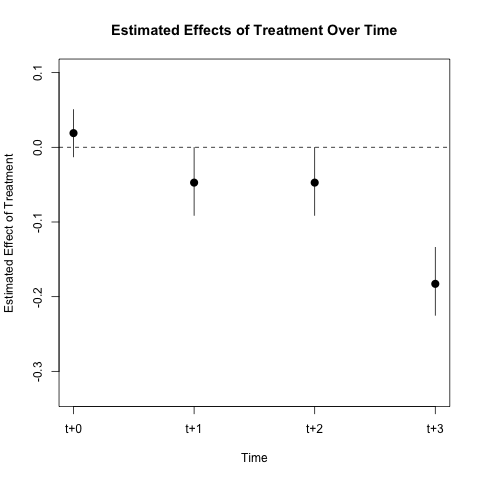
\includegraphics[width=0.9\textwidth]{../Figures/acuerdo_gobestatal.png}
       \captionsetup{justification=centering}
       
        
 \textbf{Note:} Figure \ref{fig:matching} produced by propensity score matching that adjust for the treatment and covariate histories during the 5 year periods prior to the treatment. I report 95\% bootstrap confidence intervals clustered at the state level. Covariates include those used to generate Figure \ref{fig:event_study_agreements}. 

\end{figure}   
 
\begin{figure}[H] 
\centering
 \caption{Effect of Term Limit Reform on Security Cooperation Agreements signed with the Governor, 2010-2018}
 \label{fig:chaisemarting_agreements}
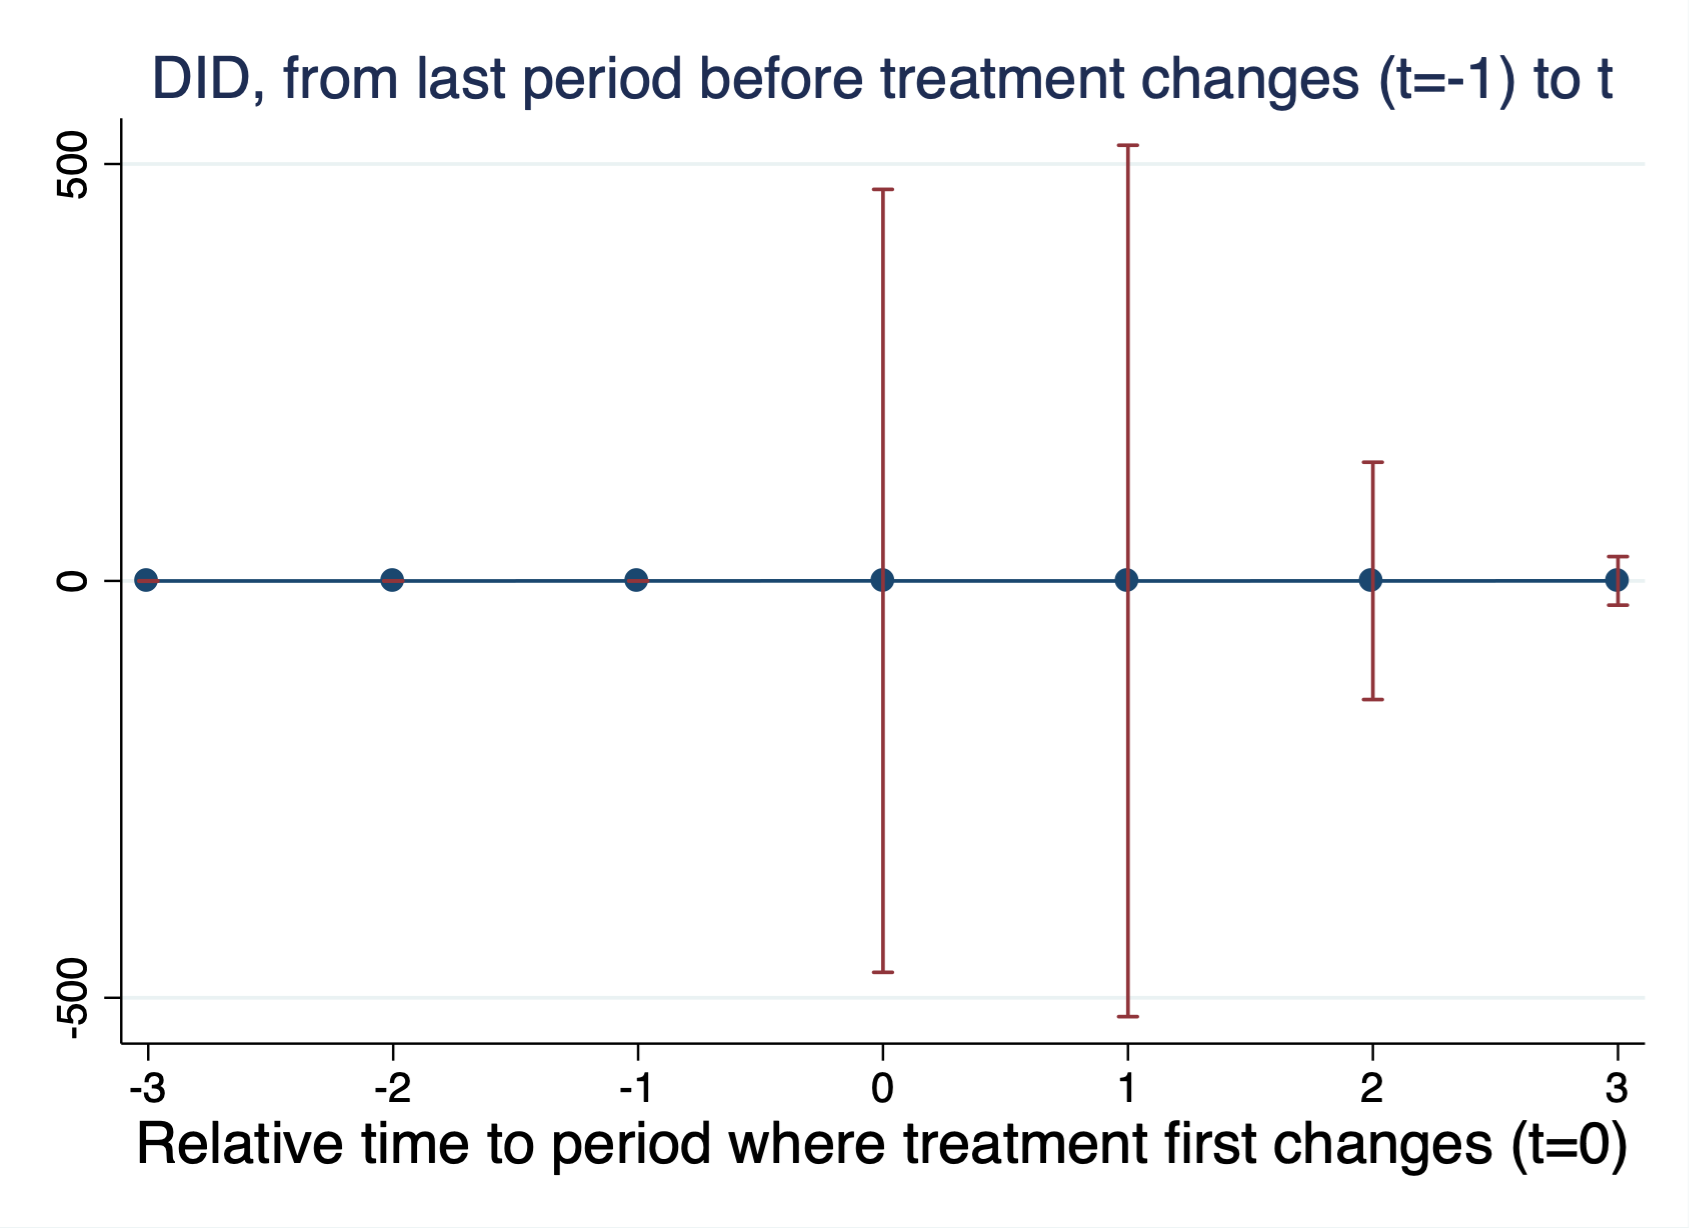
\includegraphics[width=0.9\textwidth]{../Figures/chaisemartin_acuerdo_estcom.png}
       \captionsetup{justification=centering}
\end{figure}   

  %\begin{table}[htbp]\def\sym#1{\ifmmode^{#1}\else\(^{#1}\)\fi}
\centering
\caption{Comparison: Security Cooperation Agreements with Governor vs. Other Actors, 2014-2018}
\label{tab:as_comparison_agreements}
\scalebox{1}{
\begin{tabular}{lcc}
\hline \hline
\\ \multicolumn{3}{l}{Dependent variable: Security Cooperation Agreement}\\
& w/ Governor &  w/ Other Political Actors$^a$\\
& \multicolumn{1}{c}{(1)} & \multicolumn{1}{c}{(2)} \\
\cmidrule(lrr){2-2}  \cmidrule(lrr){3-3}\\
\addlinespace
Lag 4 years &         $ 0.0197^{} $ &      $ -0.0326^{} $  \\
& ($ 0.3292$) & ($ 0.0763 $) \\
Lag 3 years &        $ -0.0102^{***} $ &     $ 0.2193^{} $ \\
& ($ 0.0000$) & ($ 0.2702 $) \\
Lag 2 years &        $ 0.1418^{} $ &    $ -0.0648^{} $  \\
& ($ 0.1318$) & ($ 0.0524 $) \\
Reform, time 0 &        $ 0.0064^{} $ &     $ -0.0089^{} $ \\
& ($ 0.0354$) & ($ 0.0069 $) \\
Lead 1 year &         $ -0.2230^{***} $ &       $ -0.2858^{} $ \\
& ($ 0.0435$) & ($ 0.2610 $) \\
Lead 3 years &        $ -0.5921^{***} $ &     $ 0.1665^{} $ \\
& ($ 0.0708$) & ($ 0.1040 $) \\
\addlinespace
Observations       &                  4,382        &           4,382  \\
R-squared        &              0.6434        &           0.5469   \\
Mun. FEs       &     \checkmark         &  \checkmark    \\
Year. FEs       &     \checkmark         &  \checkmark   \\
Controls$^b$   &      \checkmark       &      \checkmark    \\
Cohort weighted   &   \checkmark       &   \checkmark    \\
WILD CI   &          &       \\
Aggregate effect        &              $-0.2696^{***} $$         &            $0.0796^{} $$   \\
SE (aggregate eff.)        &              (0.0339)       &           (0.0491)   \\
\hline \hline
\multicolumn{3}{p{0.7\textwidth}}{\footnotesize{Notes: Coefficients show IW estimators following \citet{abraham_sun_2020}. Two relative time periods (lag 5 and 1) are removed to avoid collinearity problems noted by \citet{abraham_sun_2020}. Standard errors in parentheses are clustered at the state level, with the following significance-level: $^{***}$ 1\%; $^{**}$ 5\%; and $^*$ 10\%, that refer to two-sided t-test with the null hypothesis equal to 0 for each relative time period. $^a$ Refers primarily to the President but could include Governors and mayors from other states or other municipalities from the same state. $^b$ Pretreatment controls include: governor winning margin; party alignment with the President;  party alignment with the Governor; municipal winning margin; logged population; logged organized crime related deaths; and Cartel presence.}} \\
\end{tabular}
}
\end{table}
   
  
  \begin{table}[htbp]\def\sym#1{\ifmmode^{#1}\else\(^{#1}\)\fi}
\centering
\caption{Effect of 2014 Term Limit Reform on the likelihood of signing Security Cooperation Agreements,  by type}
\label{tab:comparison_fed_estatal}
\scalebox{1}{
\begin{tabular}{lcccc}
\hline \hline
\\ \multicolumn{3}{l}{Dependent variable:}\\
& \multicolumn{2}{c}{Security Cooperation Agreement w/ Governor$^{a}$} & \multicolumn{2}{c}{Security Cooperation Agreement w/ Other$^{b}$} \\
& \multicolumn{1}{c}{(1)} & \multicolumn{1}{c}{(2)} & \multicolumn{1}{c}{(3)} & \multicolumn{1}{c}{(4)} \\
\cmidrule(lrr){2-3}  \cmidrule(lrr){4-5}\\
\addlinespace
t-4 &         $ 0.3497^{} $ &         $ 0.0193^{} $ &     $ -0.2763^{} $ &   $ -0.0326^{} $  \\
& ($ 1.8038$) & ($ 0.3316$) & ($ 0.5842$)  & ($ 0.0761 $) \\
t-3 &         $ -0.7355^{} $ &        $ -0.0102^{***} $  &     $ 0.2469^{} $ &     $ 0.2206^{} $ \\
& ($ 37.4159$) & ($ 0.0000$) & ($ 15.0281$) & ($ 0.2702 $) \\
t-2 &         $ 0.3861^{} $ &        $ 0.1420^{} $  &     $ -0.1496^{} $ &    $ -0.0649^{} $  \\
& ($ 0.3279$) & ($ 0.1323$) & ($ 0.1250$) & ($ 0.0524 $) \\
Reform (t=0) &         $ 0.2233^{***} $ &        $ 0.0065^{} $  &     $ -0.0599^{**} $  &     $ -0.0089^{} $ \\
& ($ 0.0581$) & ($ 0.0353$) & ($ 0.0273$) & ($ 0.0070 $) \\
t+1 &         $ -0.2198^{**} $ &         $ -0.2230^{***} $  &     $ 0.1148^{} $ &       $ -0.2845^{} $ \\
& ($ 0.0930$) & ($ 0.0435$) & ($ 0.0904$) & ($ 0.2602 $) \\
t+3 &         $ -0.5915^{***} $ &        $ -0.5921^{***} $ &     $ 0.1660^{*} $  &     $ 0.1665^{} $ \\
& ($ 0.0783$) & ($ 0.0708$) & ($ 0.0953$) & ($ 0.1040 $) \\
\addlinespace
Observations   &                  4,382     &                  4,382  &                  4,382        &           4,382  \\
R-squared      &              0.6433    &              0.6434   &            0.5469        &           0.5469   \\
Mun. FEs       &     \checkmark         &  \checkmark   &     \checkmark         &  \checkmark   \\
Year. FEs       &     \checkmark         &  \checkmark  &     \checkmark         &  \checkmark   \\
Controls$^b$   &      \checkmark       &      \checkmark   &      \checkmark       &      \checkmark   \\
Cohort weighted   &          &   \checkmark   &          &   \checkmark   \\
WILD CI  &     \checkmark         &  \checkmark   &     \checkmark         &  \checkmark   \\
Aggregate effect     &              $-0.213^{***} $$    &        $-0.2696^{***} $$      &            $0.069^{} $$   &       $0.0796^{} $$   \\
SE (aggregate eff.)      &              0.034   &              0.0339    &              0.045       &           0.0491   \\
\hline \hline
\multicolumn{5}{p{1.2\textwidth}}{\footnotesize{Notes: Coefficients in columns (2) and (4) show IW estimators following \citet{abraham_sun_2020}. In those models, two relative time periods (lag 8 and 1) are removed to avoid collinearity problems noted by \citet{abraham_sun_2020}. Standard errors in parentheses are clustered at the state level, with the following significance-level: $^{***}$ 1\%; $^{**}$ 5\%; and $^*$ 10\%, that refer to two-sided t-test with the null hypothesis equal to 0 for each relative time period. $^a$ Refers to security cooperation agreements signed with the governor only. $^b$ Refers to security cooperation agreements signed with other instituions but not the governor. $^c$ State-level controls include governor winning margin in last pre-treatment election and an indicator of whether the governor's party is the same as the federal incumbent party.}} \\
\end{tabular}
}
\end{table}
   
 
 
\def\sym#1{\ifmmode^{#1}\else\(^{#1}\)\fi}
\begin{table}[htbp]\def\sym#1{\ifmmode^{#1}\else\(^{#1}\)\fi}
\centering
\caption{Test on selection on unobservables}
\label{tab:unobservables}
\begin{tabular}{l*{1}{c}}
\hline \hline
&\multicolumn{1}{c}{(1)}         \\
\addlinespace
Fitted value&      0.1312         \\
            &    (0.0780)         \\
\addlinespace
Observations&      10,668         \\
R2          &       0.459         \\
Mun. FE     &      \checkmark               \\
Year FE     &      \checkmark               \\
State Cluster S.E.&     \checkmark                \\
\hline \hline 
\multicolumn{2}{p{0.6\textwidth}}{\footnotesize{Notes: I follow \citet{altonji_etal_2005} to check if unobserved variation is likely to explain the signing of security cooperation agreements with the Governor by mayors. To do so, I regress the treatment (whether the municipality held reelection) on all the available covariates used for Figure \ref{fig:event_study_agreements}.} I then take the fitted value from the regression and use it to predict each outcome, this time including unit and year fixed effects. This test suggests that – under the assumption that observables are representative of unobservables – selection on unobservables is not driving the results.} \\
\end{tabular}
\end{table} 

\clearpage 

\begin{figure}[H]
\centering
\caption{``Event-by-event analysis'' following \citet{cengiz_etal_2019}\\ -95\% confidence intervals-} 
\label{fig:CDLZ_agreements}
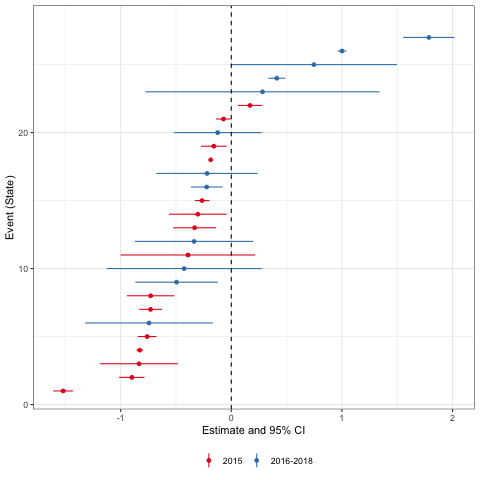
\includegraphics[width=0.75\textwidth]{../Figures/CDLZ_cov_acuerdo.png}
       \captionsetup{justification=centering}
       \\
 {\textbf Note:} Estimate separate treatment effects for each event, i.e. each Mexican state in the sample. Each event dataset contains the treated state and all other states that never received treatment or received treatment after the sample window ($t+1$).   
\end{figure}   

   
\begin{figure}[H]
\centering
\caption{``Stacked dataset analysis'' following \citet{cengiz_etal_2019}\\ -95\% confidence intervals-} 
\label{fig:stacked_wcontrols_agreements}

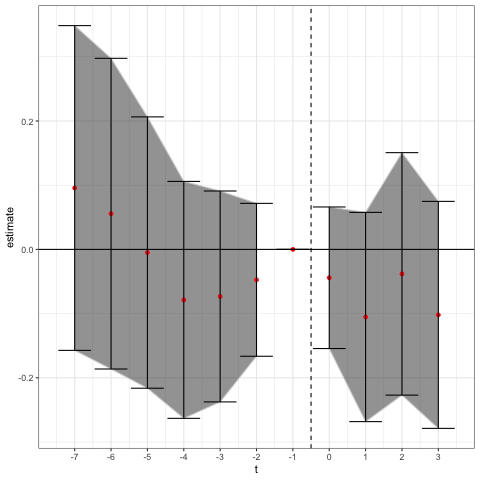
\includegraphics[width=0.75\textwidth]{../Figures/stacked_dataset_wcontrols_acuerdo.png}
       \captionsetup{justification=centering}
       \\
 {\textbf Note: Utilize estimated coefficients from Figure \ref{fig:CDLZ} and stack them in relative time, and estimate lead and lag variables to treatment following the event-by-event analysis setup, i.e. without treatment containment from using prior treated units of controls. Analysis done stacking at the cohort level, and adding municipality and year fixed effects, and clustered standard errors at the state level.}   
\end{figure}   


\begin{comment}
\begin{figure}[H]
\centering
\caption{Effect of Electoral Reform on Security Cooperation Agreement using non parametric methods\\ -95\% confidence intervals-} 
\label{fig:non_did_agreement}
\begin{center} 
\begin{center} 
	{\textbf Figure A: Generalized Synthetic Control following \citet{xu_2016} }
\end{center}
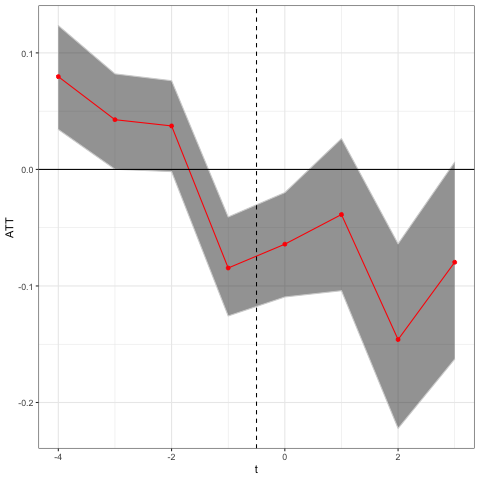
\includegraphics[width=0.55\textwidth]{../Figures/gsynth_wcov_acuerdo.png}

\begin{center}
	{\textbf Figure B: Matrix Completion following \citet{Athey, Bayati, Doudchenko, Imbens, and Khosvari}
\end{center}
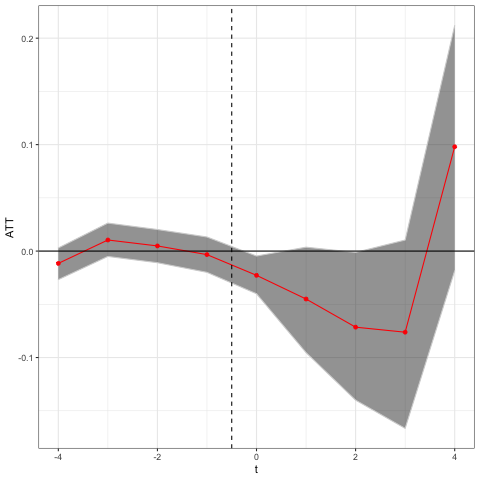
\includegraphics[width=0.55\textwidth]{Figures/matrix_completion.png}
       \captionsetup{justification=centering}
       \\
 %{\textbf Note: 95\% confidence intervals estimated using 1,000 bootstrap replications.} .   
\end{figure}      
\end{comment}


\clearpage

\subsection{Mechanisms}

\begin{figure}[H] 
\centering
 \caption{Effect of 2014 Term Limit Reform on Motives to Sign Security Agreements w/ Governor}
 \label{fig:motives}
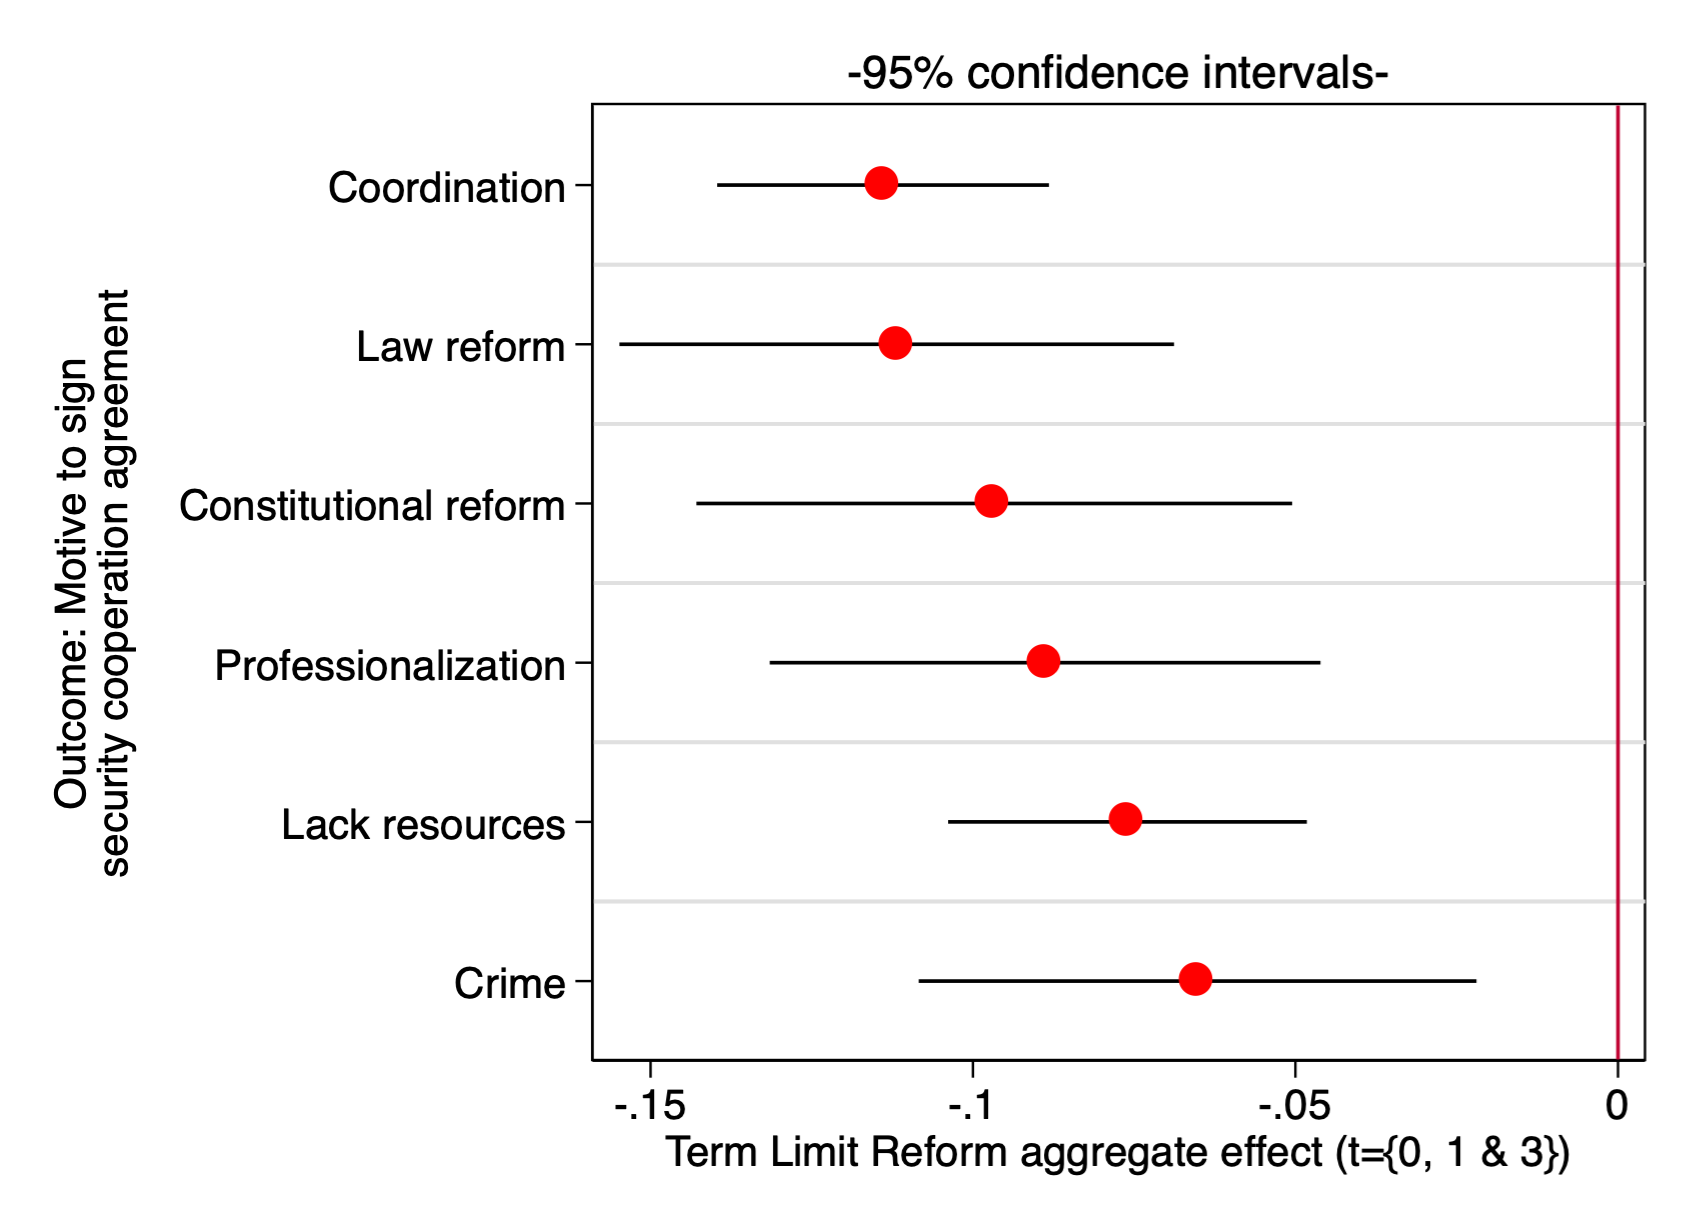
\includegraphics[width=0.9\textwidth]{../Figures/motives.png}
       \captionsetup{justification=centering}
\end{figure}   

  \begin{landscape}
\begin{table}[htbp]\def\sym#1{\ifmmode^{#1}\else\(^{#1}\)\fi}
\centering
\caption{Effect of 2014 Term Limit Reform on Motives to Sign Security Agreements w/ Governor}
\label{tab:motives_final}
\scalebox{0.70}{
\begin{tabular}{lcccccc}
\hline \hline
\\ \multicolumn{7}{l}{Dependent variable:}\\
Motive: & Cons. reform  & Law reform & Lack resources & Professionalization & Coordination & Crime \\
& \multicolumn{1}{c}{(1)} & \multicolumn{1}{c}{(2)} & \multicolumn{1}{c}{(3)} & \multicolumn{1}{c}{(4)} & \multicolumn{1}{c}{(5)} & \multicolumn{1}{c}{(6)}  \\
\cmidrule(lrr){2-2}  \cmidrule(lrr){3-3} \cmidrule(lrr){4-4} \cmidrule(lrr){5-5} \cmidrule(lrr){6-6} \cmidrule(lrr){7-7} \\
\addlinespace
t-7 &     $ -0.2350^{***} $ &     $ -0.2581^{**} $ & $ -0.0955^{*} $ & $ -0.2000^{***} $  &     $ -0.1570^{*} $   &     $ -0.1538^{} $ \\
&     ($0.0407$) &     ($0.1175$) & ($0.0484$)& ($ 0.0671$)  &    ($0.0844$)   &   ($0.1078$) \\
t-6 &     $ -0.0758^{***} $ &     $ -0.0876^{***} $ &  $ -0.0615^{***} $ &  $ -0.0647^{} $  &     $ -0.0827^{**} $ &     $ -0.0369^{} $ \\
&     ($0.0176$) &     ($0.0199$) & ($0.0162$)& ($ 0.0585$)  &    ($0.0346$)   &   ($0.0265$) \\
t-5 &     $ 0.0223^{} $ &     $ -0.0405^{} $ &  $ 0.0574^{} $ &  $ 0.0580^{} $ &     $ -0.0106^{} $  &     $ 0.0427^{} $ \\
&     ($0.0591$) &     ($0.0583$) & ($0.0481$)& ($ 0.0750$)  &    ($0.0709$)   &   ($0.0445$) \\
t-4 &     $ 0.0167^{} $ &     $ -0.0832^{} $ &   $ 0.1207^{} $ &   $ 0.0649^{} $  &     $ -0.1313^{} $ &     $ 0.0346^{} $ \\
&     ($0.0987$) &     ($0.0842$) & ($0.0854$)& ($ 0.1053$)  &    ($0.2085$)   &   ($0.1173$) \\
t-3 &     $ -0.0385^{} $ &     $ -0.0160^{} $ &   $ 0.0727^{} $ &   $ 0.0802^{} $  &     $ 0.0403^{} $ &     $ 0.0734^{} $ \\
&     ($0.1052$) &     ($0.0840$) & ($0.1002$)& ($ 0.0738$)  &    ($0.1662$)   &   ($0.1061$) \\
t-2 &     $ -0.1162^{} $ &     $ -0.0914^{} $ &  $ 0.0228^{} $  &  $ -0.0822^{} $  &     $ -0.2796^{*} $ &     $ -0.0753^{} $ \\
&     ($0.1012$) &     ($0.0917$) & ($0.0640$)& ($ 0.1195$)  &    ($0.1379$)   &   ($0.0667$) \\
Reform (t=0) &     $ 0.0457^{} $ &     $ 0.0292^{} $ &   $ 0.0214^{} $   &   $ 0.0282^{} $  &     $ 0.0233^{} $ &     $ 0.0272^{*} $ \\
&     ($0.0278$) &     ($0.0183$) & ($0.0179$)& ($ 0.0201$)  &    ($0.0209$)   &   ($0.0146$) \\
t+1 &     $ -0.0906^{***} $ &     $ -0.1071^{***} $ &    $ -0.0935^{***} $ &    $ -0.0935^{***} $ &     $ -0.1215^{***} $ &     $ -0.0735^{***} $  \\
&     ($0.0164$) &     ($0.0182$) & ($0.0106$)& ($ 0.0160$)  &    ($0.0291$)   &   ($0.0121$) \\
t+3 &     $ -0.2452^{***} $ &     $ -0.2576^{***} $ &   $ -0.1560^{***} $  &   $ -0.2011^{***} $ &     $ -0.2436^{***} $ &     $ -0.1492^{***} $ \\
&     ($0.0535$) &     ($0.0484$) & ($0.0350$)& ($ 0.0463$)  &    ($0.0431$)   &   ($0.0527$) \\
\\
\addlinespace
Observations       &              9,725    &              9,725    &           9,725      &           9,725  &              9,725    &              9,725     \\
R-squared        &          0.2974 &          0.3021    &    0.2617       &           0.2722 &          0.2865 &          0.2594      \\
Mun. FEs      &     \checkmark         &  \checkmark   &     \checkmark         &  \checkmark  &     \checkmark         &  \checkmark   &     \checkmark         &  \checkmark   \\
Year. FEs    &     \checkmark         &  \checkmark   &     \checkmark         &  \checkmark &     \checkmark         &  \checkmark   &     \checkmark         &  \checkmark   \\
Controls$^b$  &    \checkmark     &       \checkmark  &    \checkmark      &   \checkmark &    \checkmark     &       \checkmark  &    \checkmark      &   \checkmark     \\
Cohort weighted  &   \checkmark      &       \checkmark  &   \checkmark       &   \checkmark  &   \checkmark      &       \checkmark  &   \checkmark       &   \checkmark    \\
Reform aggregate effect         & $-0.0967^{***} $$      & $-0.1118^{***} $$    & $-0.0760^{***} $$      & $-0.0888^{***} $$     & $-0.1139^{***} $$      & $-0.0652^{***} $$     \\
SE       & (0.0225)  & (0.0210) & (0.0136)  & (0.0208)  & (0.0125)  & (0.0211)   \\
\hline \hline
\multicolumn{7}{p{1.2\textwidth}}{\footnotesize{Notes: Coefficients show IW estimators following \citet{abraham_sun_2020}. Two relative time periods (lag 8 and 1) are removed to avoid collinearity problems noted by \citet{abraham_sun_2020}. Standard errors in parentheses are clustered at the state level for estimates in saturaded model. Significance-level: $^{***}$ 1\%; $^{**}$ 5\%; and $^*$ 10\%, that refer to two-sided t-test with the null hypothesis equal to 0 for each relative time period. $^a$ Even columns with outcomes with missing values where replaced by zeros assuming no activity was registered. $^b$ State-level controls include governor winning margin in last pre-treatment election and an indicator of whether the governor's party is the same as the federal incumbent party.}} \\
\end{tabular}
}
\end{table}
\end{landscape}
   

   %\begin{landscape}
\begin{table}[htbp]\def\sym#1{\ifmmode^{#1}\else\(^{#1}\)\fi}
\centering
\caption{Effect of 2014 Term Limit Reform on Motives to Sign Security Agreements w/ Governor}
\label{tab:motives_average_final}
\scalebox{0.70}{
\begin{tabular}{lcccccc}
\hline \hline
\\ \multicolumn{7}{l}{Dependent variable:}\\
Motive: & Cons. reform  & Law reform & Lack resources & Professionalization & Coordination & Crime \\
& \multicolumn{1}{c}{(1)} & \multicolumn{1}{c}{(2)} & \multicolumn{1}{c}{(3)} & \multicolumn{1}{c}{(4)} & \multicolumn{1}{c}{(5)} & \multicolumn{1}{c}{(6)}  \\
\cmidrule(lrr){2-2}  \cmidrule(lrr){3-3} \cmidrule(lrr){4-4} \cmidrule(lrr){5-5} \cmidrule(lrr){6-6} \cmidrule(lrr){7-7} \\
\addlinespace
Reform average effect         & $-0.0967^{***} $$      & $-0.1118^{***} $$     & $-0.0760^{***} $$        & $-0.0888^{***} $$       & $-0.1139^{***} $$        & $-0.0652^{***} $$       \\
& (0.0225)  & (0.0210) & (0.0136)  & (0.0208)  & (0.0125)  & (0.0211)   \\
\\
\addlinespace
Observations       &              9,725    &              9,725    &           9,725      &           9,725  &              9,725    &              9,725    \\
R-squared        &          0.2974 &          0.3021    &    0.2617       &           0.2722 &          0.2865 &          0.2594   \\
Mun. FEs      &     \checkmark         &  \checkmark   &     \checkmark         &  \checkmark  &     \checkmark         &  \checkmark   &     \checkmark         &  \checkmark   \\
Year. FEs    &     \checkmark         &  \checkmark   &     \checkmark         &  \checkmark &     \checkmark         &  \checkmark   &     \checkmark         &  \checkmark   \\
Controls$^b$  &    \checkmark     &       \checkmark  &    \checkmark      &   \checkmark &    \checkmark     &       \checkmark  &    \checkmark      &   \checkmark     \\
Cohort weighted  &   \checkmark      &       \checkmark  &   \checkmark       &   \checkmark  &   \checkmark      &       \checkmark  &   \checkmark       &   \checkmark    \\
Parallel trend holds &   \checkmark      &       \checkmark  &   \checkmark       &   \checkmark  &   \checkmark      &       \checkmark  &   \checkmark       &   \checkmark    \\
\hline \hline
\multicolumn{7}{p{1.2\textwidth}}{\footnotesize{Notes: Coefficients show IW estimators following \citet{abraham_sun_2020}. Two relative time periods (lag 8 and 1) are removed to avoid collinearity problems noted by \citet{abraham_sun_2020}. Standard errors in parentheses are clustered at the state level for estimates in saturaded model. Significance-level: $^{***}$ 1\%; $^{**}$ 5\%; and $^*$ 10\%, that refer to two-sided t-test with the null hypothesis equal to 0 for each relative time period. $^a$ Even columns with outcomes with missing values where replaced by zeros assuming no activity was registered. $^b$ State-level controls include governor winning margin in last pre-treatment election and an indicator of whether the governor's party is the same as the federal incumbent party.}} \\
\end{tabular}
}
\end{table}
\end{landscape}
  
   
   
   
\begin{landscape}
\begin{table}[htbp]\def\sym#1{\ifmmode^{#1}\else\(^{#1}\)\fi}
\centering
\caption{Effect of 2014 Term Limit Reform on Services Delegated to the Governor}
\label{tab:services}
\scalebox{0.70}{
\begin{tabular}{lcccccccc}
\hline \hline
\\ \multicolumn{9}{l}{Dependent variable:}\\
Service delegated: & Public security  & Traffic & Prevention & Training  & Technology & Research & Inteligence & Unify procedures \\
& \multicolumn{1}{c}{(1)} & \multicolumn{1}{c}{(2)} & \multicolumn{1}{c}{(3)} & \multicolumn{1}{c}{(4)} & \multicolumn{1}{c}{(5)} & \multicolumn{1}{c}{(6)} & \multicolumn{1}{c}{(7)} & \multicolumn{1}{c}{(8)} \\
\cmidrule(lrr){2-2}  \cmidrule(lrr){3-3} \cmidrule(lrr){4-4} \cmidrule(lrr){5-5} \cmidrule(lrr){6-6} \cmidrule(lrr){7-7} \cmidrule(lrr){8-8} \cmidrule(lrr){9-9} \\
\addlinespace
t-2 &     $ -0.0244^{} $ &     $ -0.0441^{} $ &  $ -0.0598^{***} $  &  $ -0.0565^{***} $  &     $ -0.0567^{***} $ &     $ -0.0596^{***} $ & $ -0.0596^{***} $ & $ -0.0506^{***} $   \\
&     ($0.1046$) &     ($0.0818$) & ($0.0021$)& ($ 0.0012$)  &    ($0.0016$)   &   ($0.0017$) \\
Reform (t=0) &     $ 0.0702^{} $ &     $ 0.0256^{} $ &   $ 0.0175^{} $   &   $ 0.0214^{} $  &     $ 0.0194^{} $ &     $ 0.0194^{} $ & $ 0.0204^{} $ & $ 0.0233^{} $   \\
&     ($0.0436$) &     ($0.0369$) & ($0.0137$)& ($ 0.0142$)  &    ($0.0126$)   &   ($0.0138$) \\
t+1 &     $ -0.0947^{*} $ &     $ -0.0259^{*} $ &    $ 0.0106^{} $ &    $ 0.0053^{} $ &     $ 0.0047^{} $ &     $ 0.0024^{} $  & $ 0.0018^{} $ & $ 0.0053^{} $   \\
&     ($0.0509$) &     ($0.0147$) & ($0.0198$)& ($ 0.0193$)  &    ($0.0197$)   &   ($0.0201$) \\
t+3 &     $ -0.2847^{***} $ &     $ 0.0000^{} $  \\
&     ($0.0430$) &     ($0.0000$)  \\
\\
\addlinespace
Observations       &              4,865    &              4,865    &           3,244      &           3,244  &              3,244    &              3,244  &              3,244    &              6,481   \\
R-squared        &          0.4234 &          0.3703    &    0.5567       &           0.5477 &          0.5409 &          0.5473     &        0.5467    &        0.4894   \\
Mun. FEs      &     \checkmark         &  \checkmark   &     \checkmark         &  \checkmark  &     \checkmark         &  \checkmark   &     \checkmark         &  \checkmark   \\
Year. FEs    &     \checkmark         &  \checkmark   &     \checkmark         &  \checkmark &     \checkmark         &  \checkmark   &     \checkmark         &  \checkmark   \\
Controls$^b$  &    \checkmark     &       \checkmark  &    \checkmark      &   \checkmark &    \checkmark     &       \checkmark  &    \checkmark      &   \checkmark     \\
Cohort weighted  &   \checkmark      &       \checkmark  &   \checkmark       &   \checkmark  &   \checkmark      &       \checkmark  &   \checkmark       &   \checkmark    \\
Reform average effect         & $-0.1031^{***} $$      & $-0.0242^{} $$     & $0.0094^{} $$        & $0.0133^{} $$       & $0.0121^{} $$        & $0.0109^{} $$    & $0.0111^{} $$      & $0.0143^{} $$     \\
SE (average effect)      & (0.0225)  & (0.0162) & (0.0080)  & (0.0120)  & (0.0117)  & (0.0122)    & (0.0123)  & (0.0114)   \\
\hline \hline
\multicolumn{9}{p{1.5\textwidth}}{\footnotesize{Notes: Coefficients show IW estimators following \citet{abraham_sun_2020}. Two relative time periods (lag 8 and 1) are removed to avoid collinearity problems noted by \citet{abraham_sun_2020}. Standard errors in parentheses are clustered at the state level for estimates in saturaded model. Significance-level: $^{***}$ 1\%; $^{**}$ 5\%; and $^*$ 10\%, that refer to two-sided t-test with the null hypothesis equal to 0 for each relative time period. $^a$ Even columns with outcomes with missing values where replaced by zeros assuming no activity was registered. $^b$ State-level controls include governor winning margin in last pre-treatment election and an indicator of whether the governor's party is the same as the federal incumbent party.}} \\
\end{tabular}
}
\end{table}
\end{landscape}
   
%\begin{landscape}
\begin{table}[htbp]\def\sym#1{\ifmmode^{#1}\else\(^{#1}\)\fi}
\centering
\caption{Effect of 2014 Term Limit Reform on Services Delegated to the Governor}
\label{tab:services_average}
\scalebox{0.70}{
\begin{tabular}{lcccccccc}
\hline \hline
\\ \multicolumn{9}{l}{Dependent variable:}\\
Service delegated: & Public security  & Traffic & Prevention & Training  & Technology & Research & Inteligence & Unify procedures \\
& \multicolumn{1}{c}{(1)} & \multicolumn{1}{c}{(2)} & \multicolumn{1}{c}{(3)} & \multicolumn{1}{c}{(4)} & \multicolumn{1}{c}{(5)} & \multicolumn{1}{c}{(6)} & \multicolumn{1}{c}{(7)} & \multicolumn{1}{c}{(8)} \\
\cmidrule(lrr){2-2}  \cmidrule(lrr){3-3} \cmidrule(lrr){4-4} \cmidrule(lrr){5-5} \cmidrule(lrr){6-6} \cmidrule(lrr){7-7} \cmidrule(lrr){8-8} \cmidrule(lrr){9-9} \\
\addlinespace
Reform average effect         & $0.0149^{*} $$      & $0.0579^{***} $$     & $0.0426^{***} $$        & $0.0034^{} $$       & $-0.0345^{***} $$        & $-0.0819^{***} $$    & $0.0092^{} $$      & $0.0056^{} $$     \\
SE       & (0.0079)  & (0.0099) & (0.0046)  & (0.0048)  & (0.0103)  & (0.0085)    & (0.0063)  & (0.0034)   \\
\addlinespace
Observations       &             11,353    &             11,353    &          11,353      &          11,353  &             11,353    &             11,353  &             11,353    &             11,353   \\
R-squared        &          0.8662 &          0.8556    &    0.9239       &           0.8767 &          0.8548 &          0.8954     &        0.8557    &        0.7008   \\
Mun. FEs      &     \checkmark         &  \checkmark   &     \checkmark         &  \checkmark  &     \checkmark         &  \checkmark   &     \checkmark         &  \checkmark   \\
Year. FEs    &     \checkmark         &  \checkmark   &     \checkmark         &  \checkmark &     \checkmark         &  \checkmark   &     \checkmark         &  \checkmark   \\
Controls$^b$  &    \checkmark     &       \checkmark  &    \checkmark      &   \checkmark &    \checkmark     &       \checkmark  &    \checkmark      &   \checkmark     \\
Cohort weighted  &   \checkmark      &       \checkmark  &   \checkmark       &   \checkmark  &   \checkmark      &       \checkmark  &   \checkmark       &   \checkmark    \\
Parallel trend holds &   \checkmark      &       \checkmark  &          &     &         &       &          &       \\
\hline \hline
\multicolumn{9}{p{1.5\textwidth}}{\footnotesize{Notes: Coefficients show IW estimators following \citet{abraham_sun_2020}. Two relative time periods (lag 8 and 1) are removed to avoid collinearity problems noted by \citet{abraham_sun_2020}. Standard errors in parentheses are clustered at the state level for estimates in saturaded model. Significance-level: $^{***}$ 1\%; $^{**}$ 5\%; and $^*$ 10\%, that refer to two-sided t-test with the null hypothesis equal to 0 for each relative time period. $^a$ Even columns with outcomes with missing values where replaced by zeros assuming no activity was registered. $^b$ State-level controls include governor winning margin in last pre-treatment election and an indicator of whether the governor's party is the same as the federal incumbent party.}} \\
\end{tabular}
}
\end{table}
\end{landscape}
   

\begin{landscape}
\begin{table}[htbp]\def\sym#1{\ifmmode^{#1}\else\(^{#1}\)\fi}
\centering
\caption{Effect of 2014 Term Limit Reform on Services Delegated to the Governor}
\label{tab:interaction_alignment}
\scalebox{0.70}{
\begin{tabular}{lccc}
\hline \hline
\\ \multicolumn{4}{l}{Dependent variable: Signing Security Cooperation Agreement w/ Governor}\\
Alignment: & w/ President  & w/ Governor  & w/ Governor from PRI \\
& \multicolumn{1}{c}{(1)} & \multicolumn{1}{c}{(2)} & \multicolumn{1}{c}{(3)} \\
\cmidrule(lrr){2-2}  \cmidrule(lrr){3-3} \cmidrule(lrr){4-4} \\
\addlinespace
t-7 &     $ -0.2383^{*} $ &     $ -0.0191^{*} $ &  $ 0.0000^{} $ \\
&     ($0.1348$) &     ($0.0108$) & ($0.0000$) \\
t-6 &     $ -0.0807^{} $ &     $ 0.0199^{} $ &  $ -0.0430^{} $  \\
&     ($0.0873$) &     ($0.0499$) & ($0.0467$) \\
t-5 &     $ -0.1186^{} $ &     $ -0.2028^{**} $ &  $ -0.2406^{**} $  \\
&     ($0.1046$) &     ($0.0924$) & ($0.0922$) \\
t-4 &     $ 0.0665^{} $ &     $ -0.0784^{} $ &  $ -0.1077^{} $  \\
&     ($0.1483$) &     ($0.1203$) & ($0.1236$) \\
t-3 &     $ 0.3395^{**} $ &     $ 0.2569^{***} $ &  $ 0.2303^{***} $  \\
&     ($0.1651$) &     ($0.0720$) & ($0.0702$) \\
t-2 &     $ 0.0027^{} $ &     $ -0.0253^{} $ &  $ 0.0976^{} $  \\
&     ($0.1572$) &     ($0.1182$) & ($0.1471$) \\
Reform (t=0) &     $ -0.1686^{} $ &     $ -0.2236^{} $ &   $ 0.1790^{} $   \\
&     ($0.1877$) &     ($0.1316$) & ($0.1258$) \\
t+1 &     $ -0.2169^{} $ &     $ -0.5692^{**} $ &    $ -0.0199^{} $ \\
&     ($0.1884$) &     ($0.2119$) & ($0.1549$) \\
t+2 &     $ -0.1125^{} $ &     $ -0.5020^{*} $  &     $ -0.4753^{*} $ \\
&     ($0.2496$) &     ($0.2690$)  & ($0.2741$) \\
t+3 &     $ -0.2197^{} $ &     $ -0.3562^{} $  &     $ -0.3876^{} $ \\
&     ($0.2241$) &     ($0.3827$)  & ($0.3818$) \\
\\
\addlinespace
Observations       &             12,173    &             12,173    &          12,173    \\
R-squared        &          0.4555 &          0.4566    &    0.4541    \\
Mun. FEs      &     \checkmark         &  \checkmark   &     \checkmark    \\
Year. FEs    &     \checkmark         &  \checkmark   &     \checkmark    \\
Controls$^b$  &    \checkmark     &       \checkmark  &    \checkmark   \\
Cohort weighted  &   \checkmark      &       \checkmark  &   \checkmark    \\
Reform average effect         & $-0.1376^{} $$      & $-0.1538^{*} $$     & $-0.0551^{} $$     \\
SE (average effect)      & (0.1313)  & (0.0906) & (0.0652) \\
\hline \hline
\multicolumn{4}{p{1.5\textwidth}}{\footnotesize{Notes: Coefficients show IW estimators following \citet{abraham_sun_2020}. Two relative time periods (lag 8 and 1) are removed to avoid collinearity problems noted by \citet{abraham_sun_2020}. Standard errors in parentheses are clustered at the state level for estimates in saturaded model. Significance-level: $^{***}$ 1\%; $^{**}$ 5\%; and $^*$ 10\%, that refer to two-sided t-test with the null hypothesis equal to 0 for each relative time period. $^a$ Even columns with outcomes with missing values where replaced by zeros assuming no activity was registered. $^b$ State-level controls include governor winning margin in last pre-treatment election and an indicator of whether the governor's party is the same as the federal incumbent party.}} \\
\end{tabular}
}
\end{table}
\end{landscape}
   
%\begin{landscape}
\begin{table}[htbp]\def\sym#1{\ifmmode^{#1}\else\(^{#1}\)\fi}
\centering
\caption{Effect of 2014 Term Limit Reform on Services Delegated to the Governor}
\label{tab:interaction_alignment_average}
\scalebox{0.70}{
\begin{tabular}{lccc}
\hline \hline
\\ \multicolumn{4}{l}{Dependent variable: Signing Security Cooperation Agreement w/ Governor}\\
Alignment: & w/ President  & w/ Governor  & w/ Governor from PRI \\
& \multicolumn{1}{c}{(1)} & \multicolumn{1}{c}{(2)} & \multicolumn{1}{c}{(3)} \\
\cmidrule(lrr){2-2}  \cmidrule(lrr){3-3} \cmidrule(lrr){4-4} \\
\addlinespace
Reform average effect         & $-0.1376^{} $$      & $-0.1538^{*} $$     & $-0.0551^{} $$     \\
& (0.1313)  & (0.0906) & (0.0652) \\
\\
\addlinespace
Observations       &             12,173    &             12,173    &          12,173    \\
R-squared        &          0.4555 &          0.4566    &    0.4541    \\
Mun. FEs      &     \checkmark         &  \checkmark   &     \checkmark    \\
Year. FEs    &     \checkmark         &  \checkmark   &     \checkmark    \\
Controls$^b$  &    \checkmark     &       \checkmark  &    \checkmark   \\
Cohort weighted  &   \checkmark      &       \checkmark  &   \checkmark    \\
\hline \hline
\multicolumn{4}{p{1.5\textwidth}}{\footnotesize{Notes: Coefficients show IW estimators following \citet{abraham_sun_2020}. Two relative time periods (lag 8 and 1) are removed to avoid collinearity problems noted by \citet{abraham_sun_2020}. Standard errors in parentheses are clustered at the state level for estimates in saturaded model. Significance-level: $^{***}$ 1\%; $^{**}$ 5\%; and $^*$ 10\%, that refer to two-sided t-test with the null hypothesis equal to 0 for each relative time period. $^a$ Even columns with outcomes with missing values where replaced by zeros assuming no activity was registered. $^b$ State-level controls include governor winning margin in last pre-treatment election and an indicator of whether the governor's party is the same as the federal incumbent party.}} \\
\end{tabular}
}
\end{table}
\end{landscape}
   

        
\begin{landscape}
\begin{table}[htbp]\def\sym#1{\ifmmode^{#1}\else\(^{#1}\)\fi}
\centering
\caption{Effect of 2014 Term Limit Reform on Services Delegated to the Governor}
\label{tab:interaction_trust}
\scalebox{0.70}{
\begin{tabular}{lcccccccc}
\hline \hline
\\ \multicolumn{9}{l}{Dependent variable: Signing Security Cooperation Agreement w/ Governor}\\
Jurisdiction: & \multicolumn{2}{c}{Municipal} & \multicolumn{2}{c}{State} & \multicolumn{4}{c}{Federal} \\
Police force: & Traffic  & Preventive  & State Police & State Attorney Police & Federal Police & Ministerial Police & Army & Marines \\
& \multicolumn{1}{c}{(1)} & \multicolumn{1}{c}{(2)} & \multicolumn{1}{c}{(3)} & \multicolumn{1}{c}{(4)} & \multicolumn{1}{c}{(5)} & \multicolumn{1}{c}{(6)} & \multicolumn{1}{c}{(7)} & \multicolumn{1}{c}{(8)} \\
\cmidrule(lrr){2-2}  \cmidrule(lrr){3-3} \cmidrule(lrr){4-4} \cmidrule(lrr){5-5} \cmidrule(lrr){6-6} \cmidrule(lrr){7-7} \cmidrule(lrr){8-8} \cmidrule(lrr){9-9} \\
\addlinespace
t-7 &     $ 0.1781^{} $ &     $ 0.0000^{} $ &  $ 0.1737^{} $  &  $ 0.1270^{} $  &     $ 0.0908^{} $ &     $ 0.1162^{} $ & $ 0.1093^{*} $ & $ 0.0788^{} $   \\
&     ($0.1657$) &     ($0.0000$) & ($0.1372$)& ($ 0.1137$)  &    ($0.0736$)   &   ($0.0858$) \\
t-6 &     $ -0.0459^{} $ &     $ -0.0601^{} $ &  $ -0.0414^{} $  &  $ -0.0565^{} $  &     $ 0.0055^{} $ &     $ -0.0537^{} $ & $ 0.0234^{} $ & $ 0.0038^{} $   \\
&     ($0.0801$) &     ($0.0481$) & ($0.0539$)& ($ 0.0457$)  &    ($0.0390$)   &   ($0.0379$) \\
t-5 &     $ -0.8924^{***} $ &     $ -0.2958^{} $ &  $ -0.7754^{} $  &  $ -1.3246^{} $  &     $ -0.8583^{**} $ &     $ -1.3844^{***} $ & $ -0.6699^{**} $ & $ -0.5789^{} $   \\
&     ($0.2538$) &     ($0.2470$) & ($0.6291$)& ($ 0.9127$)  &    ($0.3310$)   &   ($0.2853$) \\
t-4 &     $ -0.8387^{} $ &     $ -0.4847^{} $ &  $ -0.8341^{} $  &  $ -1.8134^{} $  &     $ -1.0918^{} $ &     $ -1.2394^{} $ & $ -0.3796^{} $ & $ -0.4926^{} $   \\
&     ($0.7688$) &     ($0.7827$) & ($0.7594$)& ($ 1.3210$)  &    ($0.7492$)   &   ($1.0419$) \\
t-3 &     $ -0.0581^{} $ &     $ -0.2251^{} $ &  $ -0.4852^{} $  &  $ -1.8471^{} $  &     $ -0.6960^{} $ &     $ -0.8290^{} $ & $ 0.1192^{} $ & $ -0.1124^{} $   \\
&     ($0.8135$) &     ($0.8597$) & ($0.7511$)& ($ 1.3390$)  &    ($0.8562$)   &   ($1.1144$) \\
t-2 &     $ 0.0341^{} $ &     $ -0.2671^{} $ &  $ -0.2891^{} $  &  $ -0.6196^{} $  &     $ -0.6138^{} $ &     $ -0.3468^{} $ & $ -0.4246^{} $ & $ -0.4023^{} $   \\
&     ($0.5384$) &     ($0.5922$) & ($0.4176$)& ($ 0.8966$)  &    ($0.4795$)   &   ($0.7851$) \\
Reform (t=0) &     $ -0.4444^{} $ &     $ 0.1161^{} $ &   $ -0.5432^{} $   &   $ -0.3590^{} $  &     $ -1.2942^{**} $ &     $ -0.8581^{} $ & $ -0.4514^{} $ & $ -0.8446^{} $   \\
&     ($0.4490$) &     ($0.4975$) & ($0.4116$)& ($ 1.1629$)  &    ($0.5674$)   &   ($0.7678$) \\
t+1 &     $ -0.9836^{} $ &     $ -0.2186^{} $ &    $ -1.3877^{**} $ &    $ -1.3449^{} $ &     $ -2.4941^{***} $ &     $ -1.8551^{*} $  & $ -1.5407^{**} $ & $ -1.8918^{**} $   \\
&     ($0.5947$) &     ($0.5769$) & ($0.6053$)& ($ 1.4393$)  &    ($0.7475$)   &   ($0.9449$) \\
t+2 &     $ -1.8506^{***} $ &     $ -1.6311^{**} $  \\
&     ($0.5938$) &     ($0.6871$)  \\
t+3 &     $ -0.1376^{} $ &     $ -1.5275^{} $  \\
&     ($1.1164$) &     ($1.1456$)  \\
\\
\addlinespace
Observations       &             12,173    &             12,173    &          12,173      &          12,173  &             12,173    &             12,173  &             12,173    &             12,173   \\
R-squared        &          0.4666 &          0.4641    &    0.4675       &           0.4673 &          0.4642 &          0.4719     &        0.4666    &        0.4666   \\
Mun. FEs      &     \checkmark         &  \checkmark   &     \checkmark         &  \checkmark  &     \checkmark         &  \checkmark   &     \checkmark         &  \checkmark   \\
Year. FEs    &     \checkmark         &  \checkmark   &     \checkmark         &  \checkmark &     \checkmark         &  \checkmark   &     \checkmark         &  \checkmark   \\
Controls$^b$  &    \checkmark     &       \checkmark  &    \checkmark      &   \checkmark &    \checkmark     &       \checkmark  &    \checkmark      &   \checkmark     \\
Cohort weighted  &   \checkmark      &       \checkmark  &   \checkmark       &   \checkmark  &   \checkmark      &       \checkmark  &   \checkmark       &   \checkmark    \\
Reform average effect         & $-0.1399^{} $$      & $-0.2053^{} $$     & $-0.3431^{**} $$        & $-0.2984^{**} $$       & $-0.5738^{**} $$        & $-0.2614^{**} $$    & $-0.4633^{} $$      & $-0.4835^{*} $$     \\
SE (average effect)      & (0.0944)  & (0.1633) & (0.1594)  & (0.1455)  & (0.2673)  & (0.1107)    & (0.4247)  & (0.2373)   \\
\hline \hline
\multicolumn{9}{p{1.5\textwidth}}{\footnotesize{Notes: Coefficients show IW estimators following \citet{abraham_sun_2020}. Two relative time periods (lag 8 and 1) are removed to avoid collinearity problems noted by \citet{abraham_sun_2020}. Standard errors in parentheses are clustered at the state level for estimates in saturaded model. Significance-level: $^{***}$ 1\%; $^{**}$ 5\%; and $^*$ 10\%, that refer to two-sided t-test with the null hypothesis equal to 0 for each relative time period. $^a$ Even columns with outcomes with missing values where replaced by zeros assuming no activity was registered. $^b$ State-level controls include governor winning margin in last pre-treatment election and an indicator of whether the governor's party is the same as the federal incumbent party.}} \\
\end{tabular}
}
\end{table}
\end{landscape}
   
%\begin{landscape}
\begin{table}[htbp]\def\sym#1{\ifmmode^{#1}\else\(^{#1}\)\fi}
\centering
\caption{Reform interaction with citizens' preferences}
\label{tab:interaction_trust_average}
\scalebox{0.70}{
\begin{tabular}{lcccccccc}
\hline \hline
\\ \multicolumn{9}{l}{Dependent variable: Signing Security Cooperation Agreement w/ Governor}\\
Jurisdiction: & \multicolumn{2}{c}{Municipal} & \multicolumn{2}{c}{State} & \multicolumn{4}{c}{Federal} \\
Trust in Police Force: & Traffic  & Preventive  & State Police & State Attorney Police & Federal Police & Ministerial Police & Army & Marines \\
& \multicolumn{1}{c}{(1)} & \multicolumn{1}{c}{(2)} & \multicolumn{1}{c}{(3)} & \multicolumn{1}{c}{(4)} & \multicolumn{1}{c}{(5)} & \multicolumn{1}{c}{(6)} & \multicolumn{1}{c}{(7)} & \multicolumn{1}{c}{(8)} \\
\cmidrule(lrr){2-2}  \cmidrule(lrr){3-3} \cmidrule(lrr){4-4} \cmidrule(lrr){5-5} \cmidrule(lrr){6-6} \cmidrule(lrr){7-7} \cmidrule(lrr){8-8} \cmidrule(lrr){9-9} \\
\addlinespace
Reform average effect         & $-0.1400^{} $$      & $-0.2053^{} $$     & $-0.3431^{**} $$        & $-0.2984^{**} $$       & $-0.5739^{**} $$        & $-0.2614^{**} $$    & $-0.4636^{} $$      & $-0.4837^{*} $$     \\
SE (average effect)      & (0.0944)  & (0.1633) & (0.1594)  & (0.1455)  & (0.2673)  & (0.1107)    & (0.4248)  & (0.2374)   \\
\\
\addlinespace
Observations       &             12,173    &             12,173    &          12,173      &          12,173  &             12,173    &             12,173  &             12,173    &             12,173   \\
R-squared        &          0.4666 &          0.4641    &    0.4675       &           0.4673 &          0.4642 &          0.4719     &        0.4666    &        0.4666   \\
Mun. FEs      &     \checkmark         &  \checkmark   &     \checkmark         &  \checkmark  &     \checkmark         &  \checkmark   &     \checkmark         &  \checkmark   \\
Year. FEs    &     \checkmark         &  \checkmark   &     \checkmark         &  \checkmark &     \checkmark         &  \checkmark   &     \checkmark         &  \checkmark   \\
Controls$^b$  &    \checkmark     &       \checkmark  &    \checkmark      &   \checkmark &    \checkmark     &       \checkmark  &    \checkmark      &   \checkmark     \\
Cohort weighted  &   \checkmark      &       \checkmark  &   \checkmark       &   \checkmark  &   \checkmark      &       \checkmark  &   \checkmark       &   \checkmark    \\
\hline \hline
\multicolumn{9}{p{1.5\textwidth}}{\footnotesize{Notes: Coefficients show IW estimators following \citet{abraham_sun_2020}. Two relative time periods (lag 8 and 1) are removed to avoid collinearity problems noted by \citet{abraham_sun_2020}. Standard errors in parentheses are clustered at the state level, with the following significance-level: $^{***}$ 1\%; $^{**}$ 5\%; and $^*$ 10\%, that refer to two-sided t-test with the null hypothesis equal to 0 for each relative time period. $^a$ Refers to security cooperation agreements signed with the Governor. $^b$ Pretreatment controls include: governor winning margin; party alignment with the President;  party alignment with the Governor; municipal winning margin; logged population; logged organized crime related deaths; and Cartel presence.}} \\
\end{tabular}
}
\end{table}
\end{landscape}
   
 
\begin{landscape}
\begin{table}[htbp]\def\sym#1{\ifmmode^{#1}\else\(^{#1}\)\fi}
\centering
\caption{Reform interaction with citizens' being able to identify a Police Force}
\label{tab:interaction_identify}
\scalebox{0.70}{
\begin{tabular}{lcccccccc}
\hline \hline
\\ \multicolumn{9}{l}{Dependent variable: Signing Security Cooperation Agreement w/ Governor}\\
Jurisdiction: & \multicolumn{2}{c}{Municipal} & \multicolumn{2}{c}{State} & \multicolumn{4}{c}{Federal} \\
Identify Policy Force: & Traffic  & Preventive  & State Police & State Attorney Police & Federal Police & Ministerial Police & Army & Marines \\
& \multicolumn{1}{c}{(1)} & \multicolumn{1}{c}{(2)} & \multicolumn{1}{c}{(3)} & \multicolumn{1}{c}{(4)} & \multicolumn{1}{c}{(5)} & \multicolumn{1}{c}{(6)} & \multicolumn{1}{c}{(7)} & \multicolumn{1}{c}{(8)} \\
\cmidrule(lrr){2-2}  \cmidrule(lrr){3-3} \cmidrule(lrr){4-4} \cmidrule(lrr){5-5} \cmidrule(lrr){6-6} \cmidrule(lrr){7-7} \cmidrule(lrr){8-8} \cmidrule(lrr){9-9} \\
\addlinespace
t-7 &     $ -0.8572^{} $ &     $ 0.1007^{} $ &  $ 0.0649^{} $  &  $ 0.0783^{} $  &     $ -2.5321^{***} $ &     $ 0.0632^{} $ & $ -1.4640^{*} $ & $ 0.0539^{} $   \\
&     ($0.6544$) &     ($0.0978$) & ($0.0611$)& ($ 0.0697$)  &    ($0.8962$)   &   ($0.0550$) &    ($0.8372$)   &   ($0.0455$) \\
t-6 &     $ -0.2641^{} $ &     $ 0.0248^{} $ &  $ 0.0135^{} $  &  $ 0.0056^{} $  &     $ -0.7692^{***} $ &     $ -0.0035^{} $ & $ -0.4466^{*} $ & $ 0.0092^{} $   \\
&     ($0.2039$) &     ($0.0609$) & ($0.0467$)& ($ 0.0441$)  &    ($0.2696$)   &   ($0.0413$) &    ($0.2577$)   &   ($0.0423$) \\
t-5 &     $ -0.4097^{} $ &     $ -0.0652^{} $ &  $ 0.6451^{} $  &  $ 0.1762^{} $  &     $ -1.1340^{**} $ &     $ -0.7691^{***} $ & $ -0.8805^{} $ & $ -0.3720^{} $   \\
&     ($0.3986$) &     ($0.3080$) & ($0.3960$)& ($ 0.4004$)  &    ($0.4306$)   &   ($0.2589$) &    ($0.5274$)   &   ($0.2421$) \\
t-4 &     $ 0.3350^{} $ &     $ 0.1050^{} $ &  $ 0.7461^{} $  &  $ -0.0893^{} $  &     $ -1.6040^{***} $ &     $ -0.2211^{} $ & $ -0.7589^{} $ & $ -0.3294^{} $   \\
&     ($0.5455$) &     ($0.5451$) & ($0.4774$)& ($ 0.6583$)  &    ($0.5716$)   &   ($0.7553$) &    ($0.8538$)   &   ($0.4995$) \\
t-3 &     $ 0.8549^{} $ &     $ 0.3354^{} $ &  $ 0.8618^{*} $  &  $ -0.1098^{} $  &     $ -1.2530^{**} $ &     $ 0.2973^{} $ & $ -0.3261^{} $ & $ -0.0407^{} $   \\
&     ($0.5572$) &     ($0.6384$) & ($0.5038$)& ($ 0.7313$)  &    ($0.6065$)   &   ($0.8187$) &    ($0.8829$)   &   ($0.5638$) \\
t-2 &     $ -0.0741^{} $ &     $ 0.0173^{} $ &  $ 0.3106^{} $  &  $ -0.0035^{} $  &     $ -1.1572^{**} $ &     $ -0.2290^{} $ & $ -0.7416^{} $ & $ -0.3552^{} $   \\
&     ($0.3985$) &     ($0.3426$) & ($0.3583$)& ($ 0.4741$)  &    ($0.4705$)   &   ($0.5458$) &    ($0.5501$)   &   ($0.3444$) \\
Reform (t=0) &     $ 0.0965^{} $ &     $ -0.3095^{} $ &   $ -0.6740^{} $   &   $ -0.0176^{} $  &     $ -1.7122^{***} $ &     $ -0.3017^{} $ & $ -0.8230^{} $ & $ -0.7614^{} $   \\
&     ($0.3746$) &     ($0.5580$) & ($0.5072$)& ($ 0.5448$)  &    ($0.5196$)   &   ($0.5185$) &    ($0.5125$)   &   ($0.4724$) \\
t+1 &     $ 0.1452^{} $ &     $ -0.8415^{} $ &    $ -0.5733^{} $ &    $ -0.5894^{} $ &     $ -1.1449^{**} $ &     $ -1.2316^{} $  & $ -0.8753^{} $ & $ -1.6442^{***} $   \\
&     ($0.4015$) &     ($0.7920$) & ($0.6386$)& ($ 0.7035$)  &    ($0.4877$)   &   ($0.7296$) &    ($0.5560$)   &   ($0.5433$) \\
t+2 &     $ 0.4499^{} $ &     $ -0.7212^{} $ &    $ 0.0862^{} $ &    $ -1.4956^{**} $ &     $ -0.5687^{} $ &     $ -1.6626^{**} $  & $ -0.4091^{} $ & $ -1.5000^{**} $   \\
&     ($0.3760$) &     ($0.7799$) & ($0.6272$)& ($ 0.7215$)  &    ($0.5955$)   &   ($0.6266$) &    ($0.6311$)   &   ($0.5652$) \\
t+3 &     $ 1.1277^{} $ &     $ -0.5739^{} $ &    $ -0.6702^{} $ &    $ -1.2519^{} $ &     $ -1.7933^{} $ &     $ 0.0623^{} $  & $ -0.5981^{} $ & $ -1.0885^{} $   \\
&     ($0.9218$) &     ($1.2931$) & ($0.9352$)& ($ 1.0598$)  &    ($1.0758$)   &   ($1.0916$) &    ($0.9325$)   &   ($0.9434$) \\
\\
\addlinespace
Observations       &             12,173    &             12,173    &          12,173      &          12,173  &             12,173    &             12,173  &             12,173    &             12,173   \\
R-squared        &          0.4688 &          0.4599    &    0.4659       &           0.4658 &          0.4624 &          0.4783     &        0.4645    &        0.4655   \\
Mun. FEs      &     \checkmark         &  \checkmark   &     \checkmark         &  \checkmark  &     \checkmark         &  \checkmark   &     \checkmark         &  \checkmark   \\
Year. FEs    &     \checkmark         &  \checkmark   &     \checkmark         &  \checkmark &     \checkmark         &  \checkmark   &     \checkmark         &  \checkmark   \\
Controls$^b$  &    \checkmark     &       \checkmark  &    \checkmark      &   \checkmark &    \checkmark     &       \checkmark  &    \checkmark      &   \checkmark     \\
Cohort weighted  &   \checkmark      &       \checkmark  &   \checkmark       &   \checkmark  &   \checkmark      &       \checkmark  &   \checkmark       &   \checkmark    \\
Reform average effect         & $0.3037^{} $      & $-0.4471^{} $     & $-0.2964^{} $        & $-0.3087^{} $       & $-0.7782^{**} $        & $-0.2768^{} $    & $-0.5017^{} $      & $-0.5781^{**} $     \\
SE (average effect)      & (0.3233)  & (0.6044) & (0.3716)  & (0.2401)  & (0.2868)  & (0.2411)    & (0.4665)  & (0.2669)   \\
\hline \hline
\multicolumn{9}{p{1.6\textwidth}}{\footnotesize{Notes: Coefficients show IW estimators following \citet{abraham_sun_2020}. Two relative time periods (lag 8 and 1) are removed to avoid collinearity problems noted by \citet{abraham_sun_2020}. Standard errors in parentheses are clustered at the state level, with the following significance-level: $^{***}$ 1\%; $^{**}$ 5\%; and $^*$ 10\%, that refer to two-sided t-test with the null hypothesis equal to 0 for each relative time period. $^a$ Refers to security cooperation agreements signed with the Governor. $^b$ Pretreatment controls include: governor winning margin; party alignment with the President;  party alignment with the Governor; municipal winning margin; logged population; logged organized crime related deaths; and Cartel presence.}} \\
\end{tabular}
}
\end{table}
\end{landscape}
   
%\begin{landscape}
\begin{table}[htbp]\def\sym#1{\ifmmode^{#1}\else\(^{#1}\)\fi}
\centering
\caption{Reform interaction with citizens' being able to identify a Police Force}
\label{tab:interaction_identify_average}
\scalebox{0.70}{
\begin{tabular}{lcccccccc}
\hline \hline
\\ \multicolumn{9}{l}{Dependent variable: Signing Security Cooperation Agreement w/ Governor}\\
Jurisdiction: & \multicolumn{2}{c}{Municipal} & \multicolumn{2}{c}{State} & \multicolumn{4}{c}{Federal} \\
Identify Policy Force: & Traffic  & Preventive  & State Police & State Attorney Police & Federal Police & Ministerial Police & Army & Marines \\
& \multicolumn{1}{c}{(1)} & \multicolumn{1}{c}{(2)} & \multicolumn{1}{c}{(3)} & \multicolumn{1}{c}{(4)} & \multicolumn{1}{c}{(5)} & \multicolumn{1}{c}{(6)} & \multicolumn{1}{c}{(7)} & \multicolumn{1}{c}{(8)} \\
\cmidrule(lrr){2-2}  \cmidrule(lrr){3-3} \cmidrule(lrr){4-4} \cmidrule(lrr){5-5} \cmidrule(lrr){6-6} \cmidrule(lrr){7-7} \cmidrule(lrr){8-8} \cmidrule(lrr){9-9} \\
\addlinespace
Reform average effect         & $0.3037^{} $$      & $-0.4471^{} $$     & $-0.2964^{} $$        & $-0.3087^{} $$       & $-0.7782^{**} $$        & $-0.2768^{} $$    & $-0.5017^{} $$      & $-0.5781^{**} $$     \\
SE (average effect)      & (0.3233)  & (0.6044) & (0.3716)  & (0.2401)  & (0.2868)  & (0.2411)    & (0.4665)  & (0.2669)   \\
\\
\addlinespace
Observations       &             12,173    &             12,173    &          12,173      &          12,173  &             12,173    &             12,173  &             12,173    &             12,173   \\
R-squared        &          0.4688 &          0.4599    &    0.4659       &           0.4658 &          0.4624 &          0.4783     &        0.4645    &        0.4655   \\
Mun. FEs      &     \checkmark         &  \checkmark   &     \checkmark         &  \checkmark  &     \checkmark         &  \checkmark   &     \checkmark         &  \checkmark   \\
Year. FEs    &     \checkmark         &  \checkmark   &     \checkmark         &  \checkmark &     \checkmark         &  \checkmark   &     \checkmark         &  \checkmark   \\
Controls$^b$  &    \checkmark     &       \checkmark  &    \checkmark      &   \checkmark &    \checkmark     &       \checkmark  &    \checkmark      &   \checkmark     \\
Cohort weighted  &   \checkmark      &       \checkmark  &   \checkmark       &   \checkmark  &   \checkmark      &       \checkmark  &   \checkmark       &   \checkmark    \\
\hline \hline
\multicolumn{9}{p{1.6\textwidth}}{\footnotesize{Notes: Coefficients show IW estimators following \citet{abraham_sun_2020}. Two relative time periods (lag 8 and 1) are removed to avoid collinearity problems noted by \citet{abraham_sun_2020}. Standard errors in parentheses are clustered at the state level, with the following significance-level: $^{***}$ 1\%; $^{**}$ 5\%; and $^*$ 10\%, that refer to two-sided t-test with the null hypothesis equal to 0 for each relative time period. $^a$ Refers to security cooperation agreements signed with the Governor. $^b$ Pretreatment controls include: governor winning margin; party alignment with the President;  party alignment with the Governor; municipal winning margin; logged population; logged organized crime related deaths; and Cartel presence.}} \\
\end{tabular}
}
\end{table}
\end{landscape}
   
  
 \begin{landscape}
\begin{table}[htbp]\def\sym#1{\ifmmode^{#1}\else\(^{#1}\)\fi}
\centering
\caption{Reform interaction with citizens' efficiency evaluation of police forces}
\label{tab:interaction_identify}
\scalebox{0.70}{
\begin{tabular}{lcccccccc}
\hline \hline
\\ \multicolumn{9}{l}{Dependent variable: Signing Security Cooperation Agreement w/ Governor}\\
Jurisdiction: & \multicolumn{2}{c}{Municipal} & \multicolumn{2}{c}{State} & \multicolumn{4}{c}{Federal} \\
Efficiency Policy Force: & Traffic  & Preventive  & State Police & State Attorney Police & Federal Police & Ministerial Police & Army & Marines \\
& \multicolumn{1}{c}{(1)} & \multicolumn{1}{c}{(2)} & \multicolumn{1}{c}{(3)} & \multicolumn{1}{c}{(4)} & \multicolumn{1}{c}{(5)} & \multicolumn{1}{c}{(6)} & \multicolumn{1}{c}{(7)} & \multicolumn{1}{c}{(8)} \\
\cmidrule(lrr){2-2}  \cmidrule(lrr){3-3} \cmidrule(lrr){4-4} \cmidrule(lrr){5-5} \cmidrule(lrr){6-6} \cmidrule(lrr){7-7} \cmidrule(lrr){8-8} \cmidrule(lrr){9-9} \\
\addlinespace
t-7 &     $ 0.1495^{} $ &     $ 0.0000^{} $ &  $ 0.1580^{} $  &  $ 0.1178^{} $  &     $ 0.0821^{} $ &     $ 0.1125^{} $ & $ 0.0996^{} $ & $ 0.0723^{} $   \\
&     ($0.1280$) &     ($0.0000$) & ($0.1237$)& ($ 0.1059$)  &    ($0.0677$)   &   ($0.0823$) &    ($0.0592$)   &   ($0.0533$) \\
t-6 &     $ -0.0430^{} $ &     $ -0.0600^{} $ &  $ -0.0408^{} $  &  $ -0.0550^{} $  &     $ 0.0050^{} $ &     $ -0.0539^{} $ & $ 0.0218^{} $ & $ 0.0031^{} $   \\
&     ($0.0554$) &     ($0.0481$) & ($0.0487$)& ($ 0.0432$)  &    ($0.0413$)   &   ($0.0372$) &    ($0.0432$)   &   ($0.0431$) \\
t-5 &     $ -0.8214^{***} $ &     $ -0.2661^{} $ &  $ -0.6765^{} $  &  $ -1.0574^{} $  &     $ -0.8511^{**} $ &     $ -1.3151^{***} $ & $ -0.6265^{*} $ & $ -0.5477^{} $   \\
&     ($0.2173$) &     ($0.2280$) & ($0.5991$)& ($ 0.8293$)  &    ($0.3265$)   &   ($0.2946$) &    ($0.3331$)   &   ($0.3312$) \\
t-4 &     $ -0.5218^{} $ &     $ -0.3094^{} $ &  $ -0.6839^{} $  &  $ -1.4607^{} $  &     $ -1.0699^{} $ &     $ -1.1764^{} $ & $ -0.3632^{} $ & $ -0.4794^{} $   \\
&     ($0.6322$) &     ($0.6711$) & ($0.7109$)& ($ 1.2102$)  &    ($0.6659$)   &   ($0.9647$) &    ($0.5751$)   &   ($0.6316$) \\
t-3 &     $ 0.1534^{} $ &     $ -0.0826^{} $ &  $ -0.3839^{} $  &  $ -1.5521^{} $  &     $ -0.6947^{} $ &     $ -0.7613^{} $ & $ 0.1118^{} $ & $ -0.1206^{} $   \\
&     ($0.6633$) &     ($0.7380$) & ($0.6994$)& ($ 1.2330$)  &    ($0.7686$)   &   ($1.0338$) &    ($0.6450$)   &   ($0.6843$) \\
t-2 &     $ 0.1301^{} $ &     $ -0.1088^{} $ &  $ -0.2605^{} $  &  $ -0.4476^{} $  &     $ -0.6274^{} $ &     $ -0.3362^{} $ & $ -0.4306^{} $ & $ -0.4001^{} $   \\
&     ($0.4219$) &     ($0.5170$) & ($0.3883$)& ($ 0.8207$)  &    ($0.4341$)   &   ($0.7275$) &    ($0.3376$)   &   ($0.4258$) \\
Reform (t=0) &     $ -0.2825^{} $ &     $ 0.2132^{} $ &   $ -0.4068^{} $   &   $ -0.1690^{} $  &     $ -1.2332^{**} $ &     $ -0.6252^{} $ & $ -0.4515^{} $ & $ -0.8273^{} $   \\
&     ($0.3771$) &     ($0.4424$) & ($0.3661$)& ($ 1.0199$)  &    ($0.5445$)   &   ($0.7224$) &    ($0.4956$)   &   ($0.5171$) \\
t+1 &     $ -0.8544^{} $ &     $ -0.1639^{} $ &    $ -1.2047^{**} $ &    $ -1.0867^{} $ &     $ -2.4180^{***} $ &     $ -1.5837^{*} $  & $ -1.5141^{**} $ & $ -1.8447^{***} $   \\
&     ($0.5069$) &     ($0.5180$) & ($0.5515$)& ($ 1.2521$)  &    ($0.7203$)   &   ($0.9025$) &    ($0.7243$)   &   ($0.6586$) \\
t+2 &     $ -1.6548^{***} $ &     $ -1.5020^{**} $ &    $ -1.7252^{**} $ &    $ -3.6912^{***} $ &     $ -2.2110^{***} $ &     $ -3.0680^{***} $  & $ -1.1837^{} $ & $ -1.7816^{**} $   \\
&     ($0.5166$) &     ($0.6272$) & ($0.8167$)& ($ 1.0720$)  &    ($0.7669$)   &   ($0.6529$) &    ($0.7910$)   &   ($0.6492$) \\
t+3 &     $ -0.0738^{} $ &     $ -1.2495^{} $ &    $ -0.8880^{} $ &    $ -1.8369^{*} $ &     $ -1.0878^{} $ &     $ -1.0650^{} $  & $ -0.0721^{} $ & $ -1.0091^{} $   \\
&     ($0.9252$) &     ($1.0025$) & ($0.7675$)& ($ 1.0415$)  &    ($1.3469$)   &   ($1.1792$) &    ($1.2083$)   &   ($1.0552$) \\
\\
\addlinespace
Observations       &             12,173    &             12,173    &          12,173      &          12,173  &             12,173    &             12,173  &             12,173    &             12,173   \\
R-squared        &          0.4692 &          0.4656    &    0.4672       &           0.4675 &          0.4642 &          0.4725     &        0.4667    &        0.4667   \\
Mun. FEs      &     \checkmark         &  \checkmark   &     \checkmark         &  \checkmark  &     \checkmark         &  \checkmark   &     \checkmark         &  \checkmark   \\
Year. FEs    &     \checkmark         &  \checkmark   &     \checkmark         &  \checkmark &     \checkmark         &  \checkmark   &     \checkmark         &  \checkmark   \\
Controls$^b$  &    \checkmark     &       \checkmark  &    \checkmark      &   \checkmark &    \checkmark     &       \checkmark  &    \checkmark      &   \checkmark     \\
Cohort weighted  &   \checkmark      &       \checkmark  &   \checkmark       &   \checkmark  &   \checkmark      &       \checkmark  &   \checkmark       &   \checkmark    \\
Reform average effect         & $-0.1373^{} $      & $-0.1957^{} $     & $-0.3432^{*} $        & $-0.2914^{*} $       & $-0.6190^{**} $        & $-0.2679^{**} $    & $-0.5001^{} $      & $-0.5024^{**} $     \\
SE (average effect)      & (0.0917)  & (0.1697) & (0.1707)  & (0.1453)  & (0.2769)  & (0.1215)    & (0.4693)  & (0.2369)   \\
\hline \hline
\multicolumn{9}{p{1.6\textwidth}}{\footnotesize{Notes: Coefficients show IW estimators following \citet{abraham_sun_2020}. Two relative time periods (lag 8 and 1) are removed to avoid collinearity problems noted by \citet{abraham_sun_2020}. Standard errors in parentheses are clustered at the state level, with the following significance-level: $^{***}$ 1\%; $^{**}$ 5\%; and $^*$ 10\%, that refer to two-sided t-test with the null hypothesis equal to 0 for each relative time period. $^a$ Refers to security cooperation agreements signed with the Governor. $^b$ Pretreatment controls include: governor winning margin; party alignment with the President;  party alignment with the Governor; municipal winning margin; logged population; logged organized crime related deaths; and Cartel presence.}} \\
\end{tabular}
}
\end{table}
\end{landscape}
   
%\begin{landscape}
\begin{table}[htbp]\def\sym#1{\ifmmode^{#1}\else\(^{#1}\)\fi}
\centering
\caption{Effect of 2014 Term Limit Reform on Services Delegated to the Governor}
\label{tab:interaction_performance_average}
\scalebox{0.70}{
\begin{tabular}{lcccccccc}
\hline \hline
\\ \multicolumn{9}{l}{Dependent variable: Signing Security Cooperation Agreement w/ Governor}\\
Jurisdiction: & \multicolumn{2}{c}{Municipal} & \multicolumn{2}{c}{State} & \multicolumn{4}{c}{Federal} \\
Police force: & Traffic  & Preventive  & State Police & State Attorney Police & Federal Police & Ministerial Police & Army & Marines \\
& \multicolumn{1}{c}{(1)} & \multicolumn{1}{c}{(2)} & \multicolumn{1}{c}{(3)} & \multicolumn{1}{c}{(4)} & \multicolumn{1}{c}{(5)} & \multicolumn{1}{c}{(6)} & \multicolumn{1}{c}{(7)} & \multicolumn{1}{c}{(8)} \\
\cmidrule(lrr){2-2}  \cmidrule(lrr){3-3} \cmidrule(lrr){4-4} \cmidrule(lrr){5-5} \cmidrule(lrr){6-6} \cmidrule(lrr){7-7} \cmidrule(lrr){8-8} \cmidrule(lrr){9-9} \\
\addlinespace
Reform average effect         & $-0.1373^{} $$      & $-0.1957^{} $$     & $-0.3431^{*} $$        & $-0.2913^{*} $$       & $-0.6189^{**} $$        & $-0.2678^{**} $$    & $-0.4999^{} $$      & $-0.5022^{**} $$     \\
SE (average effect)      & (0.0917)  & (0.1697) & (0.1706)  & (0.1453)  & (0.2768)  & (0.1215)    & (0.4692)  & (0.2369)   \\
\\
\addlinespace
Observations       &             12,173    &             12,173    &          12,173      &          12,173  &             12,173    &             12,173  &             12,173    &             12,173   \\
R-squared        &          0.4692 &          0.4656    &    0.4672       &           0.4675 &          0.4642 &          0.4725     &        0.4667    &        0.4667   \\
Mun. FEs      &     \checkmark         &  \checkmark   &     \checkmark         &  \checkmark  &     \checkmark         &  \checkmark   &     \checkmark         &  \checkmark   \\
Year. FEs    &     \checkmark         &  \checkmark   &     \checkmark         &  \checkmark &     \checkmark         &  \checkmark   &     \checkmark         &  \checkmark   \\
Controls$^b$  &    \checkmark     &       \checkmark  &    \checkmark      &   \checkmark &    \checkmark     &       \checkmark  &    \checkmark      &   \checkmark     \\
Cohort weighted  &   \checkmark      &       \checkmark  &   \checkmark       &   \checkmark  &   \checkmark      &       \checkmark  &   \checkmark       &   \checkmark    \\
\hline \hline
\multicolumn{9}{p{1.5\textwidth}}{\footnotesize{Notes: Coefficients show IW estimators following \citet{abraham_sun_2020}. Two relative time periods (lag 8 and 1) are removed to avoid collinearity problems noted by \citet{abraham_sun_2020}. Standard errors in parentheses are clustered at the state level for estimates in saturaded model. Significance-level: $^{***}$ 1\%; $^{**}$ 5\%; and $^*$ 10\%, that refer to two-sided t-test with the null hypothesis equal to 0 for each relative time period. $^a$ Even columns with outcomes with missing values where replaced by zeros assuming no activity was registered. $^b$ State-level controls include governor winning margin in last pre-treatment election and an indicator of whether the governor's party is the same as the federal incumbent party.}} \\
\end{tabular}
}
\end{table}
\end{landscape}
 
  
  \begin{landscape}
\begin{table}[htbp]\def\sym#1{\ifmmode^{#1}\else\(^{#1}\)\fi}
\centering
\caption{Reform interaction with citizens' corruption evaluation of police forces}
\label{tab:interaction_corrupt}
\scalebox{0.70}{
\begin{tabular}{lcccccccc}
\hline \hline
\\ \multicolumn{9}{l}{Dependent variable: Signing Security Cooperation Agreement w/ Governor}\\
Jurisdiction: & \multicolumn{2}{c}{Municipal} & \multicolumn{2}{c}{State} & \multicolumn{4}{c}{Federal} \\
Corruption of Police Forces: & Traffic  & Preventive  & State Police & State Attorney Police & Federal Police & Ministerial Police & Army & Marines \\
& \multicolumn{1}{c}{(1)} & \multicolumn{1}{c}{(2)} & \multicolumn{1}{c}{(3)} & \multicolumn{1}{c}{(4)} & \multicolumn{1}{c}{(5)} & \multicolumn{1}{c}{(6)} & \multicolumn{1}{c}{(7)} & \multicolumn{1}{c}{(8)} \\
\cmidrule(lrr){2-2}  \cmidrule(lrr){3-3} \cmidrule(lrr){4-4} \cmidrule(lrr){5-5} \cmidrule(lrr){6-6} \cmidrule(lrr){7-7} \cmidrule(lrr){8-8} \cmidrule(lrr){9-9} \\
\addlinespace
t-7 &     $ 0.1477^{} $ &     $ 0.0419^{} $ &  $ 0.0402^{} $  &  $ -0.0324^{} $  &     $ -0.0147^{} $ &     $ -0.0933^{} $ & $ -0.0543^{} $ & $ -0.1444^{} $   \\
&     ($0.2864$) &     ($0.3087$) & ($0.2813$)& ($ 0.0946$)  &    ($0.3434$)   &   ($0.0782$) &    ($0.1059$)   &   ($0.1083$) \\
t-6 &     $ 0.0301^{} $ &     $ 0.0011^{} $ &  $ -0.0013^{} $  &  $ -0.0258^{} $  &     $ -0.0133^{} $ &     $ -0.0488^{} $ & $ -0.0160^{} $ & $ -0.0432^{} $   \\
&     ($0.0796$) &     ($0.1139$) & ($0.1017$)& ($ 0.0568$)  &    ($0.1316$)   &   ($0.0524$) &    ($0.0622$)   &   ($0.0617$) \\
t-5 &     $ -0.1338^{} $ &     $ -0.0973^{} $ &  $ -0.1177^{} $  &  $ -0.9190^{***} $  &     $ -0.2156^{} $ &     $ -0.8364^{***} $ & $ 0.4054^{**} $ & $ 0.4021^{**} $   \\
&     ($0.1599$) &     ($0.1895$) & ($0.1822$)& ($ 0.1316$)  &    ($0.2160$)   &   ($0.1066$) &    ($0.1573$)   &   ($0.1567$) \\
t-4 &     $ -1.3881^{***} $ &     $ -0.8179^{} $ &  $ -1.1187^{***} $  &  $ -1.3964^{***} $  &     $ -0.7440^{} $ &     $ -1.2269^{***} $ & $ 0.0944^{} $ & $ 0.3231^{} $   \\
&     ($0.3821$) &     ($0.5316$) & ($0.3690$)& ($ 0.3654$)  &    ($0.5666$)   &   ($0.3341$) &    ($0.3531$)   &   ($0.4236$) \\
t-3 &     $ -1.6818^{***} $ &     $ -0.9104^{} $ &  $ -1.2935^{***} $  &  $ -1.1282^{***} $  &     $ -0.7637^{} $ &     $ -1.0065^{***} $ & $ 0.0275^{} $ & $ 0.2564^{} $   \\
&     ($0.3568$) &     ($0.5728$) & ($0.3376$)& ($ 0.3266$)  &    ($0.6363$)   &   ($0.2992$) &    ($0.3608$)   &   ($0.4274$) \\
t-2 &     $ -0.2879^{} $ &     $ -0.2198^{} $ &  $ -0.2301^{} $  &  $ -0.9068^{***} $  &     $ -0.2657^{} $ &     $ -0.7393^{***} $ & $ 0.3265^{} $ & $ 0.3743^{} $   \\
&     ($0.2474$) &     ($0.2868$) & ($0.2681$)& ($ 0.1970$)  &    ($0.2943$)   &   ($0.1573$) &    ($0.2314$)   &   ($0.2279$) \\
Reform (t=0) &     $ -2.2651^{***} $ &     $ -1.5561^{***} $ &   $ -1.9299^{***} $   &   $ -1.0484^{***} $  &     $ -1.3274^{**} $ &     $ -0.9674^{***} $ & $ -0.8107^{***} $ & $ -0.6875^{***} $   \\
&     ($0.2832$) &     ($0.5290$) & ($0.2479$)& ($ 0.1614$)  &    ($0.5851$)   &   ($0.1417$) &    ($0.2515$)   &   ($0.2343$) \\
t+1 &     $ -3.1112^{***} $ &     $ -2.2160^{***} $ &    $ -2.6228^{***} $ &    $ -2.6054^{***} $ &     $ -1.9768^{***} $ &     $ -2.2670^{***} $  & $ -0.5640^{**} $ & $ -0.3577^{} $   \\
&     ($0.3902$) &     ($0.6501$) & ($0.3255$)& ($ 0.2394$)  &    ($0.6995$)   &   ($0.2017$) &    ($0.2557$)   &   ($0.2419$) \\
t+2 &     $ -3.0152^{***} $ &     $ -1.9965^{***} $ &    $ -2.4536^{***} $ &    $ -2.5539^{***} $ &     $ -1.7638^{**} $ &     $ -2.2646^{***} $  & $ -0.2627^{} $ & $ -0.0623^{} $   \\
&     ($0.3961$) &     ($0.6063$) & ($0.2654$)& ($ 0.2049$)  &    ($0.6524$)   &   ($0.1648$) &    ($0.2654$)   &   ($0.2224$) \\
t+3 &     $ -4.9633^{***} $ &     $ -3.2615^{***} $ &    $ -4.0463^{***} $ &    $ -2.4673^{***} $ &     $ -2.5721^{**} $ &     $ -2.2158^{***} $  & $ -1.2288^{**} $ & $ -0.9278^{**} $   \\
&     ($0.5220$) &     ($1.0612$) & ($0.3194$)& ($ 0.2057$)  &    ($1.1755$)   &   ($0.1413$) &    ($0.4848$)   &   ($0.4028$) \\
\\
\addlinespace
Observations       &             12,173    &             12,173    &          12,173      &          12,173  &             12,173    &             12,173  &             12,173    &             12,173   \\
R-squared        &          0.4593 &          0.4572    &    0.4598       &           0.4623 &          0.4636 &          0.4599     &        0.4632    &        0.4586   \\
Mun. FEs      &     \checkmark         &  \checkmark   &     \checkmark         &  \checkmark  &     \checkmark         &  \checkmark   &     \checkmark         &  \checkmark   \\
Year. FEs    &     \checkmark         &  \checkmark   &     \checkmark         &  \checkmark &     \checkmark         &  \checkmark   &     \checkmark         &  \checkmark   \\
Controls$^b$  &    \checkmark     &       \checkmark  &    \checkmark      &   \checkmark &    \checkmark     &       \checkmark  &    \checkmark      &   \checkmark     \\
Cohort weighted  &   \checkmark      &       \checkmark  &   \checkmark       &   \checkmark  &   \checkmark      &       \checkmark  &   \checkmark       &   \checkmark    \\
Reform average effect         & $-4.0564^{***} $$      & $-2.8579^{***} $$     & $-3.5587^{***} $$        & $-2.5851^{***} $$       & $-2.2583^{**} $$        & $-2.3551^{***} $$    & $-0.6132^{**} $$      & $-0.4725^{*} $$     \\
SE (average effect)      & (0.4611)  & (0.8900) & (0.3522)  & (0.2217)  & (0.9100)  & (0.1739)    & (0.2536)  & (0.2396)   \\
\hline \hline
\multicolumn{9}{p{1.6\textwidth}}{\footnotesize{Notes: Coefficients show IW estimators following \citet{abraham_sun_2020}. Two relative time periods (lag 8 and 1) are removed to avoid collinearity problems noted by \citet{abraham_sun_2020}. Standard errors in parentheses are clustered at the state level, with the following significance-level: $^{***}$ 1\%; $^{**}$ 5\%; and $^*$ 10\%, that refer to two-sided t-test with the null hypothesis equal to 0 for each relative time period. $^a$ Refers to security cooperation agreements signed with the Governor. $^b$ Pretreatment controls include: governor winning margin; party alignment with the President;  party alignment with the Governor; municipal winning margin; logged population; logged organized crime related deaths; and Cartel presence.}} \\
\end{tabular}
}
\end{table}
\end{landscape}
   
%\begin{landscape}
\begin{table}[htbp]\def\sym#1{\ifmmode^{#1}\else\(^{#1}\)\fi}
\centering
\caption{Reform interaction with citizens' corruption evaluation of police forces}
\label{tab:interaction_corrupt}
\scalebox{0.70}{
\begin{tabular}{lcccccccc}
\hline \hline
\\ \multicolumn{9}{l}{Dependent variable: Signing Security Cooperation Agreement w/ Governor}\\
Jurisdiction: & \multicolumn{2}{c}{Municipal} & \multicolumn{2}{c}{State} & \multicolumn{4}{c}{Federal} \\
Corruption of Police Forces: & Traffic  & Preventive  & State Police & State Attorney Police & Federal Police & Ministerial Police & Army & Marines \\
& \multicolumn{1}{c}{(1)} & \multicolumn{1}{c}{(2)} & \multicolumn{1}{c}{(3)} & \multicolumn{1}{c}{(4)} & \multicolumn{1}{c}{(5)} & \multicolumn{1}{c}{(6)} & \multicolumn{1}{c}{(7)} & \multicolumn{1}{c}{(8)} \\
\cmidrule(lrr){2-2}  \cmidrule(lrr){3-3} \cmidrule(lrr){4-4} \cmidrule(lrr){5-5} \cmidrule(lrr){6-6} \cmidrule(lrr){7-7} \cmidrule(lrr){8-8} \cmidrule(lrr){9-9} \\
\addlinespace
Reform average effect         & $-4.0564^{***} $$      & $-2.8579^{***} $$     & $-3.5587^{***} $$        & $-2.5851^{***} $$       & $-2.2583^{**} $$        & $-2.3551^{***} $$    & $-0.6132^{**} $$      & $-0.4725^{*} $$     \\
SE (average effect)      & (0.4611)  & (0.8900) & (0.3522)  & (0.2217)  & (0.9100)  & (0.1739)    & (0.2536)  & (0.2396)   \\
\\
\addlinespace
Observations       &             12,173    &             12,173    &          12,173      &          12,173  &             12,173    &             12,173  &             12,173    &             12,173   \\
R-squared        &          0.4593 &          0.4572    &    0.4598       &           0.4623 &          0.4636 &          0.4599     &        0.4632    &        0.4586   \\
Mun. FEs      &     \checkmark         &  \checkmark   &     \checkmark         &  \checkmark  &     \checkmark         &  \checkmark   &     \checkmark         &  \checkmark   \\
Year. FEs    &     \checkmark         &  \checkmark   &     \checkmark         &  \checkmark &     \checkmark         &  \checkmark   &     \checkmark         &  \checkmark   \\
Controls$^b$  &    \checkmark     &       \checkmark  &    \checkmark      &   \checkmark &    \checkmark     &       \checkmark  &    \checkmark      &   \checkmark     \\
Cohort weighted  &   \checkmark      &       \checkmark  &   \checkmark       &   \checkmark  &   \checkmark      &       \checkmark  &   \checkmark       &   \checkmark    \\
\hline \hline
\multicolumn{9}{p{1.6\textwidth}}{\footnotesize{Notes: Coefficients show IW estimators following \citet{abraham_sun_2020}. Two relative time periods (lag 8 and 1) are removed to avoid collinearity problems noted by \citet{abraham_sun_2020}. Standard errors in parentheses are clustered at the state level, with the following significance-level: $^{***}$ 1\%; $^{**}$ 5\%; and $^*$ 10\%, that refer to two-sided t-test with the null hypothesis equal to 0 for each relative time period. $^a$ Refers to security cooperation agreements signed with the Governor. $^b$ Pretreatment controls include: governor winning margin; party alignment with the President;  party alignment with the Governor; municipal winning margin; logged population; logged organized crime related deaths; and Cartel presence.}} \\
\end{tabular}
}
\end{table}
\end{landscape}
   
    
 \clearpage   
 
 \subsection{Unintended consequences}
 \textbf{A. Preferences}
 
   \begin{landscape}
\begin{table}[htbp]\def\sym#1{\ifmmode^{#1}\else\(^{#1}\)\fi}
\centering
\caption{Effect of 2014 Term Limit Reform on Services Delegated to the Governor}
\label{tab:preferences}
\scalebox{0.60}{
\begin{tabular}{lccccccccccc}
\hline \hline
\\ \multicolumn{12}{l}{Dependent variable: topic that worries the most}\\
& Narcotraffick & Insecurity & Punishment to criminals & Corruption  & Poverty & Unemployment & Inflation & Natural Disasters & Water Scarcity & Education & Health \\
& \multicolumn{1}{c}{(1)} & \multicolumn{1}{c}{(2)} & \multicolumn{1}{c}{(3)} & \multicolumn{1}{c}{(4)} & \multicolumn{1}{c}{(5)} & \multicolumn{1}{c}{(6)} & \multicolumn{1}{c}{(7)} & \multicolumn{1}{c}{(8)} & \multicolumn{1}{c}{(9)} & \multicolumn{1}{c}{(10)} & \multicolumn{1}{c}{(11)}\\
\cmidrule(lrr){2-2}  \cmidrule(lrr){3-3} \cmidrule(lrr){4-4} \cmidrule(lrr){5-5} \cmidrule(lrr){6-6} \cmidrule(lrr){7-7} \cmidrule(lrr){8-8} \cmidrule(lrr){9-9} \cmidrule(lrr){10-10} \cmidrule(lrr){11-11} \cmidrule(lrr){12-12}\\
\addlinespace
t-6 &     $ 0.0190^{***} $ &     $ 0.0218^{**} $ &  $ -0.0088^{} $  &  $ 0.0140^{**} $  &     $ -0.0363^{***} $ &     $ 0.0120^{} $ & $ -0.0150^{} $ & $ -0.0121^{***} $ & $ 0.0119^{*} $ & $ 0.0106^{***} $ & $ -0.0087^{***} $  \\
&     ($0.0066$) &     ($0.0085$) & ($0.0121$)& ($ 0.0060$)  &    ($0.0118$)   &   ($0.0156$) &   ($0.0103$) &   ($0.0021$) &   ($0.0066$) &   ($0.0013$) &   ($0.0022$) \\
t-5 &     $ 0.0073^{***} $ &     $ 0.0166^{**} $ &  $ 0.0062^{} $  &  $ 0.0015^{} $  &     $ -0.0186^{***} $ &     $ 0.0144^{*} $ & $ -0.0065^{} $ & $ -0.0059^{**} $ & $ -0.0038^{***} $ & $ 0.0011^{} $ & $ -0.0091^{**} $  \\
&     ($0.0012$) &     ($0.0062$) & ($0.0063$)& ($ 0.0018$)  &    ($0.0062$)   &   ($0.0073$) &   ($0.0065$) &   ($0.0025$) &   ($0.0012$) &   ($0.0009$) &   ($0.0034$) \\
t-4 &     $ -0.0034^{} $ &     $ 0.0920^{**} $ &  $ 0.0218^{} $  &  $ -0.0049^{} $  &     $ -0.0447^{} $ &     $ 0.0106^{} $ & $ -0.0431^{*} $ & $ -0.0055^{} $ & $ 0.0303^{**} $ & $ 0.0089^{} $ & $ -0.0492^{**} $  \\
&     ($0.0083$) &     ($0.0379$) & ($0.0247$)& ($ 0.0142$)  &    ($0.0273$)   &   ($0.0233$) &   ($0.0224$) &   ($0.0043$) &   ($0.0119$) &   ($0.0052$) &   ($0.0189$) \\
t-3 &     $ 0.0440^{**} $ &     $ 0.0728^{} $ &  $ -0.0034^{} $  &  $ -0.0143^{} $  &     $ -0.0276^{} $ &     $ 0.0254^{} $ & $ -0.0204^{} $ & $ 0.0015^{} $ & $ -0.0156^{} $ & $ 0.0071^{} $ & $ -0.0536^{**} $  \\
&     ($0.0182$) &     ($0.0566$) & ($0.0210$)& ($ 0.0202$)  &    ($0.0438$)   &   ($0.0332$) &   ($0.0152$) &   ($0.0116$) &   ($0.0238$) &   ($0.0172$) &   ($0.0228$) \\
t-2 &     $ 0.0280^{} $ &     $ 0.0146^{} $ &  $ 0.0305^{} $  &  $ -0.0195^{} $  &     $ -0.0255^{} $ &     $ 0.0265^{} $ & $ 0.0435^{***} $ & $ 0.0121^{} $ & $ -0.0003^{} $ & $ -0.0306^{*} $ & $ -0.0623^{*} $  \\
&     ($0.0219$) &     ($0.0497$) & ($0.0195$)& ($ 0.0217$)  &    ($0.0421$)   &   ($0.0211$) &   ($0.0143$) &   ($0.0159$) &   ($0.0171$) &   ($0.0157$) &   ($0.0314$) \\
Reform, t=0 &     $ 0.0021^{} $ &     $ 0.0267^{***} $ &  $ 0.0206^{***} $  &  $ 0.0012^{} $  &     $ -0.0187^{***} $ &     $ -0.0355^{***} $ & $ 0.0034^{} $ & $ -0.0016^{} $ & $ 0.0073^{} $ & $ -0.0091^{**} $ & $ 0.0017^{} $  \\
&     ($0.0050$) &     ($0.0072$) & ($0.0037$)& ($ 0.0044$)  &    ($0.0063$)   &   ($0.0051$) &   ($0.0056$) &   ($0.0026$) &   ($0.0052$) &   ($0.0039$) &   ($0.0053$) \\
t+1 &     $ 0.0165^{**} $ &     $ 0.0427^{***} $ &  $ 0.0270^{***} $  &  $ 0.0126^{***} $  &     $ -0.0392^{***} $ &     $ -0.0803^{***} $ & $ 0.0520^{***} $ & $ 0.0093^{} $ & $ 0.0017^{} $ & $ -0.0189^{***} $ & $ -0.0329^{***} $  \\
&     ($0.0071$) &     ($0.0112$) & ($0.0037$)& ($ 0.0045$)  &    ($0.0097$)   &   ($0.0058$) &   ($0.0075$) &   ($0.0074$) &   ($0.0053$) &   ($0.0046$) &   ($0.0071$) \\
t+2 &     $ 0.0227^{**} $ &     $ 0.0785^{***} $ &  $ 0.0400^{***} $  &  $ 0.0079^{*} $  &     $ -0.0405^{***} $ &     $ -0.1023^{***} $ & $ 0.0172^{*} $ & $ 0.0099^{*} $ & $ 0.0107^{*} $ & $ -0.0283^{***} $ & $ -0.0323^{***} $  \\
&     ($0.0086$) &     ($0.0108$) & ($0.0050$)& ($ 0.0042$)  &    ($0.0108$)   &   ($0.0087$) &   ($0.0093$) &   ($0.0050$) &   ($0.0062$) &   ($0.0062$) &   ($0.0058$) \\
t+3 &     $ 0.0182^{} $ &     $ 0.0837^{***} $ &  $ 0.0828^{***} $  &  $ -0.0081^{} $  &     $ -0.0397^{**} $ &     $ -0.1094^{***} $ & $ -0.0357^{***} $ & $ 0.0048^{*} $ & $ 0.0228^{**} $ & $ -0.0275^{***} $ & $ -0.0152^{} $  \\
&     ($0.0134$) &     ($0.0151$) & ($0.0098$)& ($ 0.0080$)  &    ($0.0169$)   &   ($0.0177$) &   ($0.0064$) &   ($0.0025$) &   ($0.0087$) &   ($0.0092$) &   ($0.0109$) \\
\\
\addlinespace
Observations       &             11,353    &             11,353    &          11,353      &          11,353  &             11,353    &             11,353  &             11,353    &             11,353  &             11,353 &             11,353  &             11,353  \\
R-squared        &          0.8662 &          0.8556    &    0.9239       &           0.8767 &          0.8548 &          0.8954     &        0.8557    &        0.7008  &        0.8419  &        0.8048  &        0.8799  \\
Mun. FEs      &     \checkmark         &  \checkmark   &     \checkmark         &  \checkmark  &     \checkmark         &  \checkmark   &     \checkmark         &  \checkmark    &  \checkmark   &     \checkmark         &  \checkmark \\
Year. FEs    &     \checkmark         &  \checkmark   &     \checkmark         &  \checkmark &     \checkmark         &  \checkmark   &     \checkmark         &  \checkmark   &  \checkmark   &     \checkmark         &  \checkmark  \\
Controls$^b$  &    \checkmark     &       \checkmark  &    \checkmark      &   \checkmark &    \checkmark     &       \checkmark  &    \checkmark      &   \checkmark     &  \checkmark   &     \checkmark         &  \checkmark  \\
Cohort weighted  &   \checkmark      &       \checkmark  &   \checkmark       &   \checkmark  &   \checkmark      &       \checkmark  &   \checkmark       &   \checkmark     &  \checkmark   &     \checkmark         &  \checkmark \\
Reform average effect         & $0.0149^{*} $$      & $0.0579^{***} $$     & $0.0426^{***} $$        & $0.0034^{} $$       & $-0.0345^{***} $$        & $-0.0819^{***} $$    & $0.0092^{} $$      & $0.0056^{} $$    & $0.0106^{**} $$   & $-0.0209^{***} $$   & $^{} $$  \\
SE (average effect)      & (0.0079)  & (0.0099) & (0.0046)  & (0.0048)  & (0.0103)  & (0.0085)    & (0.0063)  & (0.0034)   & (0.0047)   & (0.0055)   & (0.0063)  \\
\hline \hline
\multicolumn{12}{p{1.7\textwidth}}{\footnotesize{Notes: Coefficients show IW estimators following \citet{abraham_sun_2020}. Two relative time periods (lag 8 and 1) are removed to avoid collinearity problems noted by \citet{abraham_sun_2020}. Standard errors in parentheses are clustered at the state level for estimates in saturaded model. Significance-level: $^{***}$ 1\%; $^{**}$ 5\%; and $^*$ 10\%, that refer to two-sided t-test with the null hypothesis equal to 0 for each relative time period. $^a$ Even columns with outcomes with missing values where replaced by zeros assuming no activity was registered. $^b$ State-level controls include governor winning margin in last pre-treatment election and an indicator of whether the governor's party is the same as the federal incumbent party.}} \\
\end{tabular}
}
\end{table}
\end{landscape}
   
%\begin{landscape}
\begin{table}[htbp]\def\sym#1{\ifmmode^{#1}\else\(^{#1}\)\fi}
\centering
\caption{Effect of 2014 Term Limit Reform on Citizens Preferences}
\label{tab:preferences_average}
\scalebox{0.60}{
\begin{tabular}{lccccccccccc}
\hline \hline
\\ \multicolumn{12}{l}{Dependent variable: topic that worries the most}\\
& Narcotraffic & Insecurity & Punishment to criminals & Corruption  & Poverty & Unemployment & Inflation & Natural Disasters & Water Scarcity & Education & Health \\
& \multicolumn{1}{c}{(1)} & \multicolumn{1}{c}{(2)} & \multicolumn{1}{c}{(3)} & \multicolumn{1}{c}{(4)} & \multicolumn{1}{c}{(5)} & \multicolumn{1}{c}{(6)} & \multicolumn{1}{c}{(7)} & \multicolumn{1}{c}{(8)} & \multicolumn{1}{c}{(9)} & \multicolumn{1}{c}{(10)} & \multicolumn{1}{c}{(11)}\\
\cmidrule(lrr){2-2}  \cmidrule(lrr){3-3} \cmidrule(lrr){4-4} \cmidrule(lrr){5-5} \cmidrule(lrr){6-6} \cmidrule(lrr){7-7} \cmidrule(lrr){8-8} \cmidrule(lrr){9-9} \cmidrule(lrr){10-10} \cmidrule(lrr){11-11} \cmidrule(lrr){12-12}\\
\addlinespace
Reform average effect         & $0.0149^{*} $$      & $0.0579^{***} $$     & $0.0426^{***} $$        & $0.0034^{} $$       & $-0.0345^{***} $$        & $-0.0819^{***} $$    & $0.0092^{} $$      & $0.0056^{} $$    & $0.0106^{**} $$   & $-0.0209^{***} $$   & $^{} $$  \\
SE (average effect)      & (0.0079)  & (0.0099) & (0.0046)  & (0.0048)  & (0.0103)  & (0.0085)    & (0.0063)  & (0.0034)   & (0.0047)   & (0.0055)   & (0.0063)  \\
\\
\addlinespace
Observations       &             11,353    &             11,353    &          11,353      &          11,353  &             11,353    &             11,353  &             11,353    &             11,353  &             11,353 &             11,353  &             11,353  \\
R-squared        &          0.8662 &          0.8556    &    0.9239       &           0.8767 &          0.8549 &          0.8954     &        0.8557    &        0.7008  &        0.8419  &        0.8048  &        0.8799  \\
Mun. FEs      &     \checkmark         &  \checkmark   &     \checkmark         &  \checkmark  &     \checkmark         &  \checkmark   &     \checkmark         &  \checkmark    &  \checkmark   &     \checkmark         &  \checkmark \\
Year. FEs    &     \checkmark         &  \checkmark   &     \checkmark         &  \checkmark &     \checkmark         &  \checkmark   &     \checkmark         &  \checkmark   &  \checkmark   &     \checkmark         &  \checkmark  \\
Controls$^b$  &    \checkmark     &       \checkmark  &    \checkmark      &   \checkmark &    \checkmark     &       \checkmark  &    \checkmark      &   \checkmark     &  \checkmark   &     \checkmark         &  \checkmark  \\
Cohort weighted  &   \checkmark      &       \checkmark  &   \checkmark       &   \checkmark  &   \checkmark      &       \checkmark  &   \checkmark       &   \checkmark     &  \checkmark   &     \checkmark         &  \checkmark \\
\hline \hline
\multicolumn{12}{p{1.7\textwidth}}{\footnotesize{Notes: Coefficients show IW estimators following \citet{abraham_sun_2020}. Two relative time periods (lag 8 and 1) are removed to avoid collinearity problems noted by \citet{abraham_sun_2020} except for the specification that trims periods prior to t-4. Standard errors in parentheses are clustered at the state level, with the following significance-level: $^{***}$ 1\%; $^{**}$ 5\%; and $^*$ 10\%, that refer to two-sided t-test with the null hypothesis equal to 0 for each relative time period. $^b$ State-level controls include governor winning margin in last pre-treatment election and an indicator of whether the governor's party is the same as the federal incumbent party.}} \\
\end{tabular}
}
\end{table}
\end{landscape}
   
         
 
\textbf{B. Violence}

   \begin{table}[H]\def\sym#1{\ifmmode^{#1}\else\(^{#1}\)\fi}
\centering
\caption{Effect of 2014 Term Limit Reform on Violence}
\label{tab:as_homicides}
\scalebox{0.75}{
\begin{tabular}{lcc}
\hline \hline
\\ \multicolumn{3}{l}{Dependent variable:}\\
& \multicolumn{1}{c}{log(homicide per capita)} & \multicolumn{1}{c}{IHS(homicide per capita)$^{a}$} \\
& \multicolumn{1}{c}{(1)} & \multicolumn{1}{c}{(2)} \\
\cmidrule(lrr){2-2}  \cmidrule(lrr){3-3}\\
\addlinespace
Lag 6 years &          $ 0.0119^{} $ &   $ -0.1702^{} $  \\
& ($ 0.0195$) & ($ 0.1061 $) \\
Lag 5 years &        $ -0.0480^{} $ &   $ 0.0381^{} $ \\
& ($ 0.0357$) & ($ 0.0856 $) \\
Lag 4 years &         $ 0.0403^{} $ &      $ -0.0440^{} $  \\
& ($ 0.1012$) & ($ 0.2077 $) \\
Lag 3 years &        $ 0.0167^{} $ &     $ -0.0015^{} $ \\
& ($ 0.0581$) & ($ 0.1098 $) \\
Lag 2 years &        $ -0.0288^{} $ &    $ -0.1734^{} $  \\
& ($ 0.0498$) & ($ 0.1098 $) \\
Reform, time 0 &        $ 0.0024^{} $ &     $ 0.0067^{} $ \\
& ($ 0.0324$) & ($ 0.0583 $) \\
Lead 1 year &         $ 0.0719^{*} $ &       $ 0.0168^{} $ \\
& ($ 0.0401$) & ($ 0.0692 $) \\
Lead 2 years &         $ 0.1420^{***} $ &      $ 0.1814^{**} $  \\
& ($ 0.0465$) & ($ 0.0761 $) \\
Lead 3 years &        $ 0.1890^{*} $ &     $ 0.2805^{*} $ \\
& ($ 0.0993$) & ($ 0.1481 $) \\
\addlinespace
Observations       &                 12,173        &          12,173  \\
R-squared        &              0.7267        &           0.5330   \\
Mun. FEs       &     \checkmark         &  \checkmark    \\
Year. FEs       &     \checkmark         &  \checkmark   \\
Controls$^b$   &      \checkmark       &      \checkmark    \\
Cohort weighted   &   \checkmark       &   \checkmark    \\
Aggregate effect        &           $   0.1013^{**} $        &           $0.1213^{*} $    \\
SE (aggregate eff.)        &              0.0442        &           0.0687   \\
Standardize Aggregate effect        &           $   0.1036^{**} $        &           $0.0662^{*} $    \\
Standardize SE (aggregate eff.)        &              0.0452        &           0.0375   \\
\hline \hline
\multicolumn{3}{p{0.9\textwidth}}{\footnotesize{Notes: Coefficients show IW estimators following \citet{abraham_sun_2020}. Two relative time periods (lag 8 and 0) are removed to avoid collinearity problems noted by \citet{abraham_sun_2020}. Standard errors in parentheses are clustered at the state level, with the following significance-level: $^{***}$ 1\%; $^{**}$ 5\%; and $^*$ 10\%, that refer to two-sided t-test with the null hypothesis equal to 0 for each relative time period. $^a$ Inverse hyperbolic sine transformation. $^b$ Pretreatment controls include: governor winning margin; party alignment with the President;  party alignment with the Governor; municipal winning margin; and Cartel presence.}} \\
\end{tabular}
}
\end{table}
   
   
     \begin{figure}[H]   
\centering
 \caption{Robustness tests: Effect of Term Limit Reform on Violence, 2010-2018}
 \label{fig:robustness_violence}
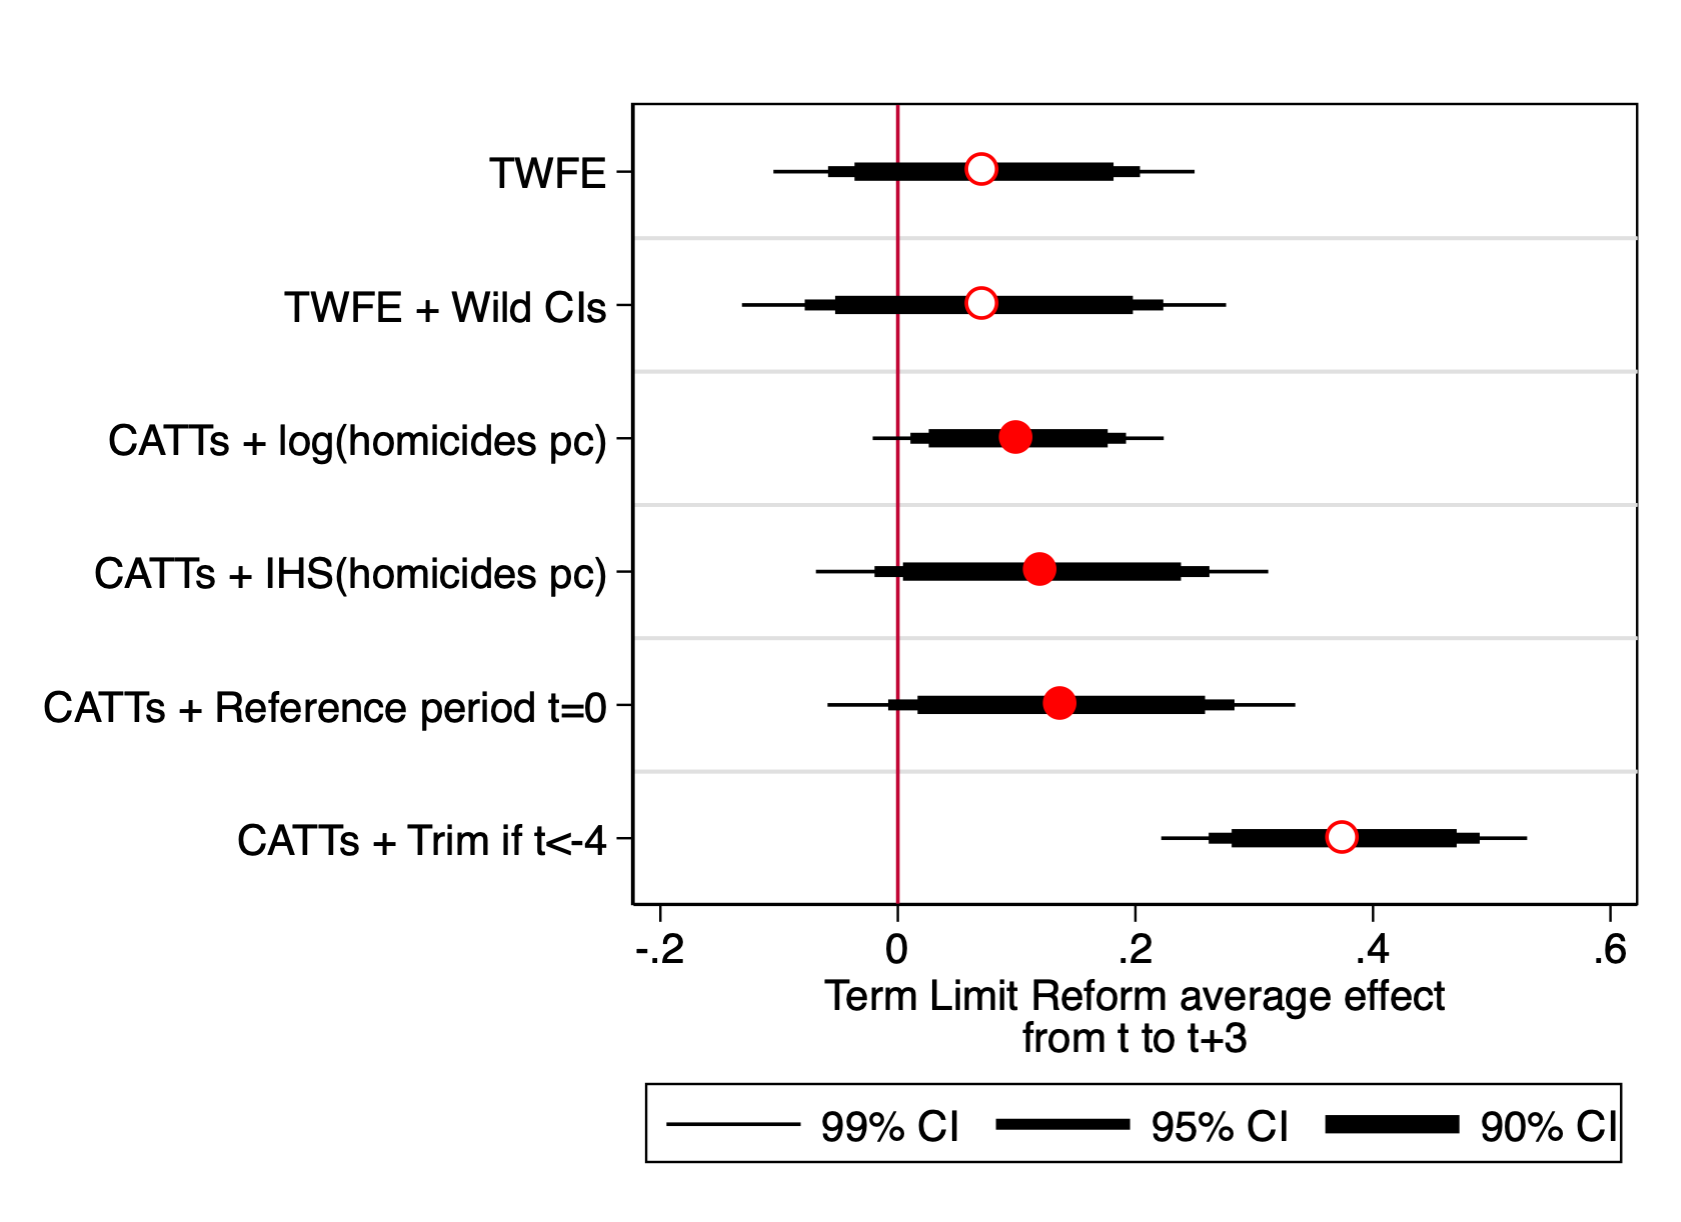
\includegraphics[width=0.9\textwidth]{../Figures/average_effects_homicides.png}
       \captionsetup{justification=centering}
       
 \textbf{Note:} Figure \ref{fig:robustness_violence} shows the average treatment effect from t to t+3 across multiple specifications. This average effect was estimated using the IW estimators following \citet{abraham_sun_2020} for each lead and lag relative to the first year a municipality implemented reelection. Red points show that parallel trends hold, while hollow ones imply pretrends. 
\end{figure}      

\begin{figure}[H] 
\centering
 \caption{Effect of Term Limit Reform on Violence, propensity score matching on pretreatment covariates}
 \label{fig:matching_violence}
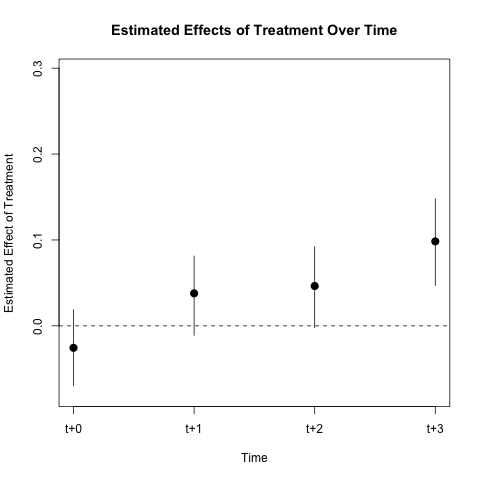
\includegraphics[width=0.75\textwidth]{../Figures/panelmatch_logdefuncionespc.png}
       \captionsetup{justification=centering}
    
        
 \textbf{Note:} Figure \ref{fig:matching_violence} produced by propensity score matching that adjust for the treatment and covariate histories during the 5 year periods prior to the treatment. I report 95\% bootstrap confidence intervals clustered at the state level. Covariates include those used to generate Figure \ref{fig:event_study_agreements}. 
 
\end{figure}   
           
    
    
 \clearpage   
            
%APPENDIX -----------------------------------------------

%%%%%%%%%%%%
\bibliographystyle{aer} 
\bibliography{References}    

\clearpage
%APPENDIX -----------------------------------------------
\begin{appendix}
\renewcommand{\thetable}{A-\arabic{table}}
\setcounter{table}{0}
 
\renewcommand{\thefigure}{B-\arabic{figure}}
\setcounter{figure}{0}

   
%%%%%%%%%%%%%%%%%%%%%%%%%%%%%%%%% 

  
\end{document}
